% Autor: Leonhard Segger, Jannik Tim Zarnitz
% Datum: 2017-10-30
\documentclass[
% Papierformat
a4paper,
% Schriftgröße (beliebige Größen mit „fontsize=Xpt“)
12pt,
% Schreibt die Papiergröße korrekt ins Ausgabedokument
pagesize,
% Sprache für z.B. Babel
ngerman
]{scrartcl}

% Achtung: Die Reihenfolge der Pakete kann (leider) wichtig sein!
% Insbesondere sollten (so wie hier) babel, fontenc und inputenc (in dieser
% Reihenfolge) als Erstes und hyperref und cleveref (Reihenfolge auch hier
% beachten) als Letztes geladen werden!

\usepackage{tikz}
\usetikzlibrary{calc,patterns,angles,quotes} % loads some tikz extensions\usepackage{tikz}
\usetikzlibrary{babel}

% Silbentrennung etc.; Sprache wird durch Option bei \documentclass festgelegt
\usepackage{babel}
% Verwendung der Zeichentabelle T1 (Sonderzeichen etc.)
\usepackage[T1]{fontenc}
% Legt die Zeichenkodierung der Eingabedatei fest, z.B. UTF-8
\usepackage[utf8]{inputenc}
% Schriftart
\usepackage{lmodern}
% Zusätzliche Sonderzeichen
\usepackage{textcomp}

% Mathepaket (intlimits: Grenzen über/unter Integralzeichen)
\usepackage[intlimits]{amsmath}
% Ermöglicht die Nutzung von \SI{Zahl}{Einheit} u.a.
\usepackage{siunitx}
% Zum flexiblen Einbinden von Grafiken (\includegraphics)
\usepackage{graphicx}
% Abbildungen im Fließtext
\usepackage{wrapfig}
% Abbildungen nebeneinander (subfigure, subtable)
\usepackage{subcaption}
% Funktionen für Anführungszeichen
\usepackage{csquotes}
\MakeOuterQuote{"}
% Zitieren, Bibliografie
\usepackage{biblatex}


% Zur Darstellung von Webadressen
\usepackage{url}
%chemische Formeln
\usepackage[version=4]{mhchem}
% siunitx: Deutsche Ausgabe, Messfehler getrennt mit ± ausgeben
\usepackage{floatrow}
\floatsetup[table]{capposition=top}
\usepackage{float}
% Verlinkt Textstellen im PDF-Dokument
\usepackage[unicode]{hyperref}
% "Schlaue" Referenzen (nach hyperref laden!)
\usepackage{cleveref}
\sisetup{
	locale=DE,
	separate-uncertainty
}
\bibliography{EIRE2018_References}

\begin{document}
	
	\begin{titlepage}
		\centering
		{\scshape\LARGE Protokoll zur \par} 
		\vspace{1cm}
		{\scshape\huge Einführung in rechnergestütztes Experimentieren \par}
		\vspace{3cm}
		
		{\large Jannik Tim Zarnitz (E-Mail: j\_zarn02@wwu.de) \par}
		{\large Leonhard Segger (E-Mail: l\_segg03@wwu.de) \par}
		\vfill
		
		in der Woche 03.09.2018 bis 06.09.2018\par
		betreut von\par
		{\large Dr. Jürgen Berkemeier}
		
		\vfill
		
		{\large \today\par}
	\end{titlepage}
	\tableofcontents
	\newpage

%TODO Deckblatt prüfen
%TODO am Ende: Begriffe vereinheitlichen und Größe von Grafiken anpassen

	\section{Aufbau einer Sinus- bzw. Bessel-Funktion} \label{sinusfkt}
	
	Zunächst soll unter Verwendung der graphischen Programmiersprache \glqq LabVIEW\grqq\ eine Sinus-Funktion realisiert werden.
	Mithilfe der von LabVIEW zur Verfügung gestellten numerischen Operationen, Konstanten und Schleifen (sogenannten \enquote{Visual Instruments} oder einfach VIs) lässt sich ein Programm schreiben, welches eine Sinusschwingung $u$ der Form
	
	\begin{equation} \label{u}
	u(A,f,t,\varphi) = A \cdot \sin(2\pi f t + \varphi) \ ,
	\end{equation}
	
	\noindent umsetzt. Wobei $A$ die Schwingungsamplitude, $f$ die Frequenz und $\varphi$ die Phasenverschiebung bilden. Außerdem ist jedes $t$ durch 
	
	\begin{equation} \label{t}
	t = \frac{i}{N}
	\end{equation}
	
	\noindent gegeben. $N$ ist dabei die Zahl der Stützstellen und zugleich die Anzahl der zu berechnenden Wertepaare. Der Index $i$ kann Werte im Bereich zwischen $0$ und $N$ annehmen. Der zugehörige Programmcode, das Blockdiagramm in LabVIEW, ist in \cref{sinusbesselprogrammcode} zu sehen. 
	
	\begin{figure}[H]
		\centering
		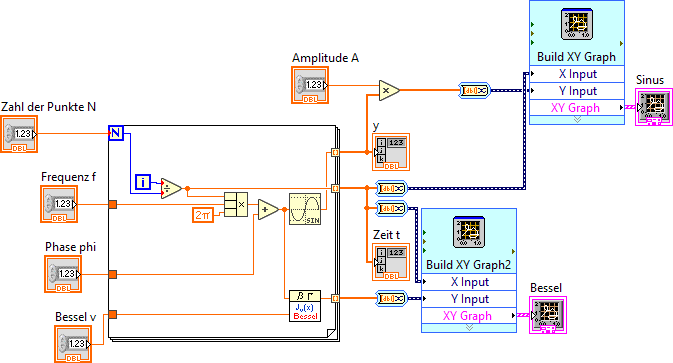
\includegraphics[width=1.0\textwidth]{EIRE2018Dateien/Tag1/sinusbessel-bilder/SinusBesseld}
		\caption{Die Abbildung zeigt ein LabVIEW-Blockdiagramm, also den Aufbau des Programms, zur Umsetzung einer Sinus- und Bessel-Funktion. Die eigentliche Berechnung findet innerhalb der For-Schleife statt. Dazu werden feste, aber beliebige Fließkommazahlen für die Amplitude $A$, die Zahl der Punkte $N$, die Frequenz $f$, die Phase $\varphi$ und die Ordnung $\nu$ der Bessel-Funktion herangezogen, nachdem sie auf der Frontplatte eingestellt wurden. Die Ausgabe der Wertepaare erfolgt in Form zweier $X$-$Y$-Graphen sowie Arrays.}
		\label{sinusbesselprogrammcode}
	\end{figure}

	\noindent Das dazugehörige ausgegebene Frontpanel ist in \cref{sinusbesselausgabe} erkennbar. Die Gleitkommazahlen-Werte für $A$, $f$, $N$ und $\varphi$ sollen frei wählbar sein, zumal $u$ insbesondere von diesen abhängt. Das Programm ist daher so eingerichtet, dass auf der linken Seite des Frontpanels die entsprechenden Bedien- bzw. Eingabeelemente erscheinen. Unter gleichem Namen sind die jeweiligen Blockdiagrammobjekte im Programmcode zu finden. Im Zentrum des Programmcodes in \cref{sinusbesselprogrammcode} lässt sich eine For-Schleife erkennen. Gemäß \cref{u} sowie \cref{t} findet in dieser unter Verwendung des Laufindexes $i$ die tatsächliche Berechnung der $t$- und $u$-Werte statt. Die Blockdiagrammobjekte auf der rechten Seite des Programmcodes in \cref{sinusbesselprogrammcode} bilden die Anzeige- bzw. Ausgabeelemente des Frontpanels in \cref{sinusbesselausgabe}. Zum einen werden dabei zwei $N+1$ Einträge umfassende, eindimensionale Arrays angelegt, die jeweils alle $t$- sowie sämtliche $u$-Werte beinhalten und zum anderen wird ein $X$-$Y$-Diagramm erzeugt, in dem alle $u$-Werte gegen die entsprechenden $t$-Werte aufgetragen sind.
	Dabei befindet sich $t$ auf der $x$-Achse und $u$ auf der $y$-Achse. 
	Um nun die Informationsübertragung zu bewerkstelligen, ist es notwendig im Programmcode vor den Anschlüssen der \glqq Build XY Graph\grqq -VIs weitere Blockdiagrammobjekte hinzuzufügen, welche das Leitungssignal in ein für das Anzeigeelement ($X$-$Y$-Diagramm) passendes Eingangssignal umwandeln. Zumeist geschieht dies in LabVIEW automatisch und wird dann an der entsprechenden Stelle auf der Leitung mit einem kleinen roten Punkt markiert.

	\begin{figure}[H]
		\centering
		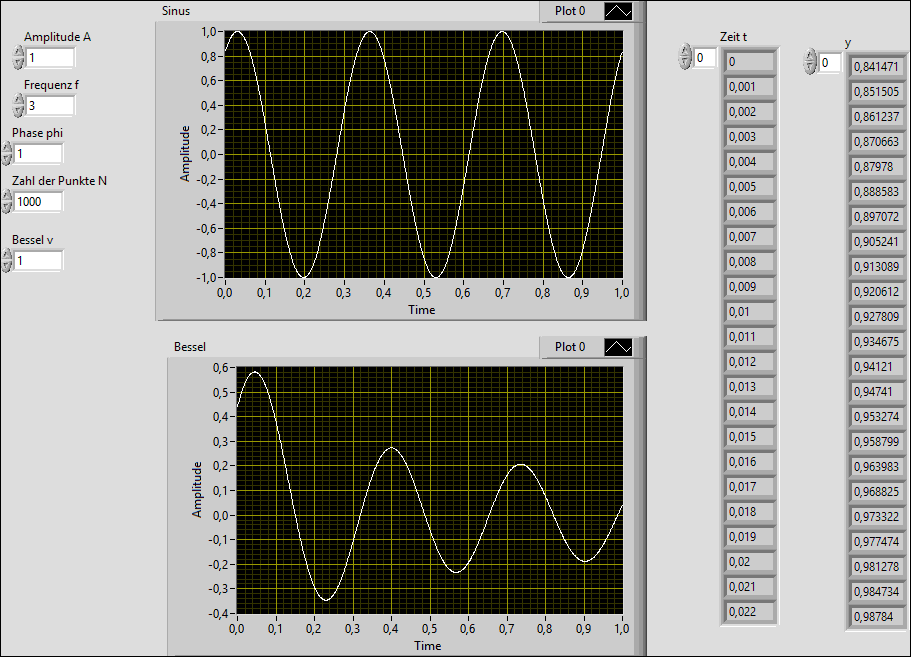
\includegraphics[width=1.0\textwidth]{EIRE2018Dateien/Tag1/sinusbessel-bilder/SinusBesselp}
		\caption{In dieser Abbildung ist das Frontpanel als Ausgabe und Benutzeroberfläche dargestellt.}
		\label{sinusbesselausgabe}
	\end{figure}

	\noindent Zusätzlich zur Sinus-Funktion wird eine Bessel-Funktion erster Gattung $J_{\nu}$ mit LabVIEW realisiert und ebenfalls in das Programm in \cref{sinusbesselprogrammcode} mit aufgenommen. Das entsprechende Blockdiagrammobjekt ist mit \glqq $J_{\nu}(x)$ Bessel\grqq\ gekennzeichnet. Die Bessel-Funktion besitzt die allgemeine Form
	
	\begin{equation}
	J_{\nu}(x) = \sum_{j=0}^{\infty}\frac{(-1)^j \cdot \left( \frac{x}{2}\right) ^{2j+\nu}}{j! \cdot \Gamma(\nu + j + 1)} \ . %das juckt niemanden. aber jetzt ists auch egal
	\end{equation}
	
	\noindent Wobei $\nu$ die Ordnung der Bessel-Funktion bildet, $\Gamma(\cdot)$ die Gamma-Funktion darstellt und $x$ auf Basis des Programmcodes in \cref{sinusbesselprogrammcode} als %eigentlich fängt man Sätze nicht mit Wobei an sondern nur Nebensätze
	
	\begin{equation}
	x := 2\pi f t + \varphi = \frac{2\pi f \cdot i}{N} + \varphi
	\end{equation}
	
	\noindent definiert ist. Der Fließkommazahlen-Wert für $\nu$ ist, ähnlich wie beim Sinus-Programm, über das entsprechende Bedienelement auf der linken Seite des Frontpanels einstellbar, was in \cref{sinusbesselausgabe} zu erkennen ist. Genauso wie beim Sinus-Programm findet die Berechnung der $x$- und $J_{\nu}(x)$-Werte innerhalb der For-Schleife statt. Die Werteausgabe erfolgt in Form eines $X$-$Y$-Diagramms, dessen Anzeigeelement im unteren Bereich der \cref{sinusbesselausgabe} ersichtlich ist und in dem $J_{\nu}(x)$ als Funktion von $x$ dargestellt ist. Zudem muss das Eingangssignal so wie zuvor beim Sinus-Programm für das dazugehörige Blockdiagrammobjekt in \cref{sinusbesselprogrammcode} passend umgewandelt werden.

	\begin{figure}[H]
		\centering
		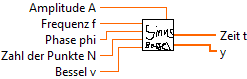
\includegraphics[width=0.5\textwidth]{EIRE2018Dateien/Tag1/sinusbessel-bilder/SinusBesselc}
		\caption{Die Abbildung zeigt das gestaltete Programm-Icon sowie die gesetzten Anschlussmöglichkeiten.}
		\label{sinusbesselicon}
	\end{figure}
	
	\noindent LabVIEW bietet die Möglichkeit ein bereits vorhandenes, selbst geschriebenes, funktionsfähiges Programm so zu bearbeiten, dass es für andere LabVIEW-Programme bzw. -Projekte als Blockdiagrammobjekt nutzbar wird. Dazu müssen zunächst die Anschlüsse sowohl die der Eingänge als auch die der  Ausgänge \enquote{verkabelt} werden. Allgemein kann es sich dabei um verschiedenste Arten von Ein-und Ausgangssignalen handeln. Bei der programmierten Sinus-Funktion verhält es sich demnach so, dass fünf Eingangs- und zwei Ausgangsanschlüsse generiert werden müssen, welche jeweils nur Gleitkommazahlen annehmen bzw. übergeben. Die Amplitude $A$, die Frequenz $f$, die Phasenverschiebung $\varphi$, die Anzahl der Punkte $N$ und die Ordnung $\nu$ der Bessel-Funktion bilden hierbei die Eingänge, die $t$-Werte sowie die $u$- bzw. $y$-Werte erscheinen über die beiden Ausgänge. Des Weiteren ist es in LabVIEW möglich das entsprechende Blockdiagrammobjekt-Icon des Programms zu gestalten. Das komplette Resultat ist in \cref{sinusbesselicon} dargestellt.
	
	\emph{Hinweis:} Aus der Betrachtung des Programmcodes in \cref{sinusbesselprogrammcode} geht hervor, dass das Blockdiagrammobjekt, welches das Array-Ausgabeelement des Frontpanels bildet und alle $u$-Werte abgreifen soll, inkorrekt eingefügt ist. Denn anstelle einer Implementierung nach der Multiplikation mit der Amplitude $A$, befindet sich das besagte Blockdiagrammobjekt davor. Sodass das Array lediglich die Werte des Ausdrucks
	
	\begin{equation}
	\sin(2\pi f t + \varphi)
	\end{equation}
	
	\noindent angibt, welche zwischen $-1$ und $1$ liegen. Da die Ausgabefunktion als Array einen erheblichen Einfluss auf das folgende Vorgehen hat, kann mit dem Sinus-Programm in dieser Form nicht weitergearbeitet werden. Im weiteren Verlauf der Projektbearbeitung ist der beschriebene Fehler allerdings behoben worden. Eine berichtigte, aktualisierte Abbildung des Programms liegt an dieser Stelle jedoch nicht vor.
	\label{sinus_amp_fehler}
	
	\newpage
	
	
	\section{Lissajous-Figuren}
	
	Im Folgenden sollen je nach Werteeinstellungen auf dem Anzeigeelement der Benutzeroberfläche verschiedene Lissajous-Figuren entstehen. Dies ist in \cref{lissajous} zu sehen. Die Basis für eine solche Lissajous-Figur bilden zwei verschiedene Sinusschwingungen, welche beide dieselbe Gestalt wie die \cref{u} besitzen:
	
	\begin{equation} \label{u1u2}
	u_1(A_1,f_1,t,\varphi_1) = A_1 \cdot \sin(2\pi f_1 t + \varphi_1) \ \ \ \textnormal{und} \ \ \ u_2(A_2,f_2,t,\varphi_2) = A_2 \cdot \sin(2\pi f_2 t + \varphi_2) \ ,
	\end{equation}
	
	\noindent mit den unterschiedlichen Amplituden $A_1$ und $A_2$, den Frequenzen $f_1$ und $f_2$ sowie den Phasenverschiebungen $\varphi_1$ und $\varphi_2$. Zudem bedarf es eines zweidimensionalen kartesischen Koordinatensystems mit Rechts- und Hochachse. Eine Lissajous-Figur entsteht nun dadurch, dass man der $x$-Achse die Funktion $u_1$ und der $y$-Achse die Funktion $u_2$ zuweist. Je nachdem wie man die Werte für $A_1$, $A_2$, $f_1$, $f_2$, $\varphi_1$, $\varphi_2$ und $N$ wählt, ergeben sich dann unterschiedliche Lissajous-Figuren.
	
	\begin{figure}[H]
		\centering
		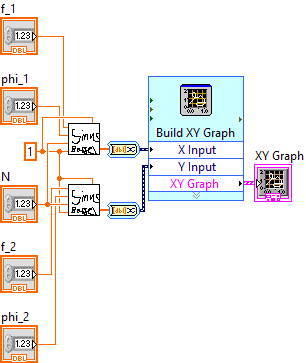
\includegraphics[width=0.6\textwidth]{EIRE2018Dateien/Tag1/lissajous-bilder/Lissajousd}
		\caption{Dargestellt ist das Blockdiagramm, also der LabVIEW-Programmcode, mit dem sich Lissajous-Figuren realisieren lassen.}
		\label{lissajousprogrammcode}
	\end{figure}

	\noindent Der dazugehörige Programmcode ist in \cref{lissajousprogrammcode} zu erkennen. Die in \cref{sinusfkt} erstellte Sinus-Funktion bildet die Grundlage, denn mit dieser lassen sich die beiden separaten Schwingungen $u_1$ und $u_2$ aus \cref{u1u2} realisieren. Dabei ist es möglich das Sinus-Programm als Blockdiagrammobjekt in den Programmcode einfügen, jeweils einmal für $u_1$ und $u_2$, was in \cref{lissajousprogrammcode} deutlich wird. An die offenen Eingangsanschlüsse müssen entsprechende, sogenannte \glqq Controls\grqq\ für die Frequenzen $f_1$ und $f_2$, für die Phasenverschiebungen $\varphi_1$ und $\varphi_2$ sowie für die Zahl der Stützstellen $N$ angeschlossen werden. Die dazugehörigen Bedien- bzw. Eingabeelemente befinden sich links auf dem Frontpanel des Programms, so wie es in \cref{lissajous} dargestellt ist. Für die Amplituden soll einfachheitshalber $A_1 = A_2 = 1$ gelten.

	\begin{figure}[H]
		\centering
		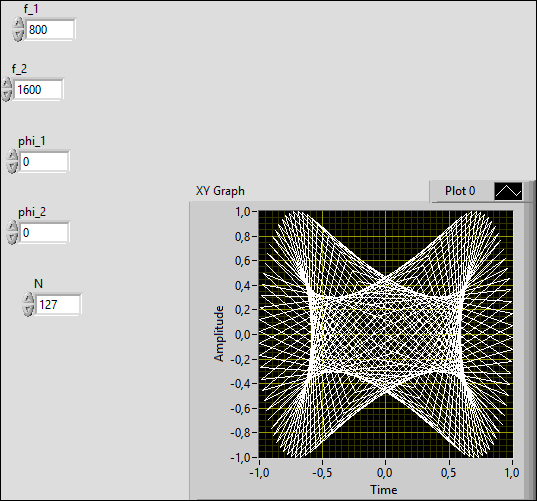
\includegraphics[width=1.0\textwidth]{EIRE2018Dateien/Tag1/lissajous-bilder/Lissajousp}
		\caption{Die Abbildung zeigt das Frontpanel bzw. die Benutzeroberfläche, in dem sich im Anzeigeelement eine Lissajous-Figur befindet. Auf der linken Seite können die entsprechenden $f_1$-, $f_2$-, $\varphi_1$-, $\varphi_2$- und $N$-Werte abgelesen werden.}
		\label{lissajous}
	\end{figure}

	\noindent An den Ausgangsanschlüssen wird ein $X$-$Y$-Diagramm angebracht, wobei die $u_1$-Werte auf der $x$-Achse und die $u_2$-Werte auf der $y$-Achse liegen. Wie beim Programm in \cref{sinusfkt}, ist dem Ausgabeelement an der entsprechenden Stelle auf der Leitung ein passendes Blockdiagrammobjekt zur Signalumwandlung vorgeschaltet. Je nach Wahl der $f_1$-, $f_2$-, $\varphi_1$-, $\varphi_2$- und $N$-Werte können sich somit die unterschiedlichsten Lissajous-Figuren formen.
	
	\newpage
	
	
	\section{Digitales Oszilloskop mit ExpressVI}
	Es wird ein Funktionsgenerator verwendet.
	Dessen Signal wird über einen Analog-Digital-Wandler durch den Computer erfasst.
	Zunächst wird das Signal in LabView mit dem entsprechenden ExpressVI verarbeitet, welches dem Nutzer große Teile des Konfigurationsvorgangs abnimmt.
	Das zugehörige Programm ist in \cref{fig_tag2_oszi_express_block} und die Frontplatte in \cref{fig_tag2_oszi_express_front} dargestellt.
	
	\begin{figure}[H]  
		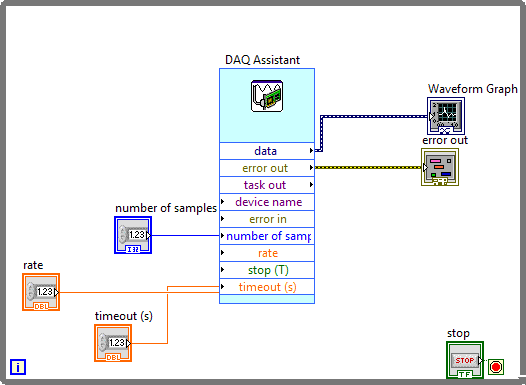
\includegraphics[width=1\textwidth]{EIRE2018Dateien/Tag2/expressVI_1d}
		\centering
		\caption{
			Einfaches Oszilloskop mithilfe des ExpressVIs zur Erfassung von Daten von Messgeräten. Das Programm erlaubt die graphische Darstellung einer Wellenform.
		}
		\label{fig_tag2_oszi_express_block}
		\centering
	\end{figure}
	\begin{figure}[H]  
		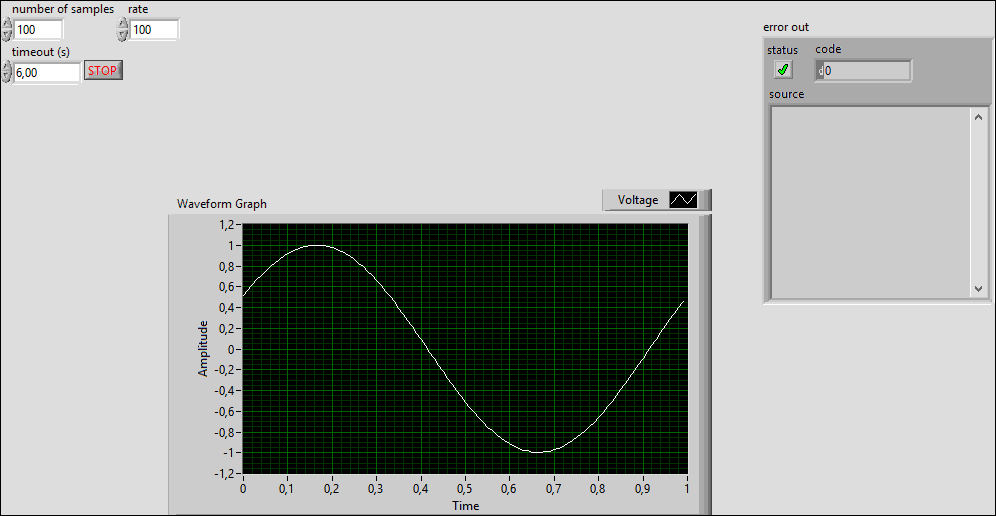
\includegraphics[width=1\textwidth]{EIRE2018Dateien/Tag2/expressVI_1p}
		\centering
		\caption{
			Frontplatte des einfachen Oszilloskop mithilfe des ExpressVIs zur Erfassung von Daten von Messgeräten. Dabei wurde durch den Funktionsgenerator ein sinusförmiges Signal ausgegeben.
		}
		\label{fig_tag2_oszi_express_front}
	\centering
	\end{figure}
	
	\newpage
	
	
	\section{Abtasten von Signalen}
	
	\subsection{Fourier-Theorem}
	Gemäß des Fourier-Theorems kann jede periodische Funktion als Fourier-Reihe bzw. Fourier-Integral ausgedrückt werden.
	Dies ist nützlich bei der Zerlegung eines möglicherweise verrauschten Signals in seine Bestandteile.
	Das grundsätzliche Problem hierbei ist, dass Messprozesse immer zeitlich begrenzt sind, weshalb das Signal nicht bis in die positive und negative Unendlichkeit periodisch sein kann.
	Dies verursacht den sogenannten \enquote{Leakage-Effekt}, auf den in \cref{leakage} näher eingegangen wird.
	
	\subsection{Abtasttheorem}
	Um ein Signal abzutasten, werden im Analog-Digital-Wandler mithilfe einer Sample-and-Hold-Schaltung zeitlich diskrete Messungen durchgeführt.
	Dies lässt sich als Multiplikation des Signals mit einem Delta-Kamm ausdrücken.
	Dabei treten Summen- und Differenzfrequenzen von Abtastfrequenz und deren Oberfrequenzen mit den Frequenzen im Signal auf.
	Im Frequenzraum ergibt sich hierdurch eine periodische Fortsetzung des Spektrums des ursprünglichen Signals, wobei die Periode der Abtastfrequenz entspricht.
	Dies ist in \cref{fig_Aliasing_veranschaulichung} veranschaulicht.
	Wenn die Abtastfrequenz hinreichend groß ist, kann man nun mithilfe eines Tiefpasses das Signal herausfiltern.
	Dazu muss sie allerdings größer als das Doppelte der höchsten im Signal auftretenden Frequenz sein, da sich ansonsten das Spektrum des Signals mit den Differenzfrequenzen der nächsten Periode überlagern.
	Wenn dies geschieht, bezeichnet man es als Aliasing.
	
	\begin{figure}[H]  
		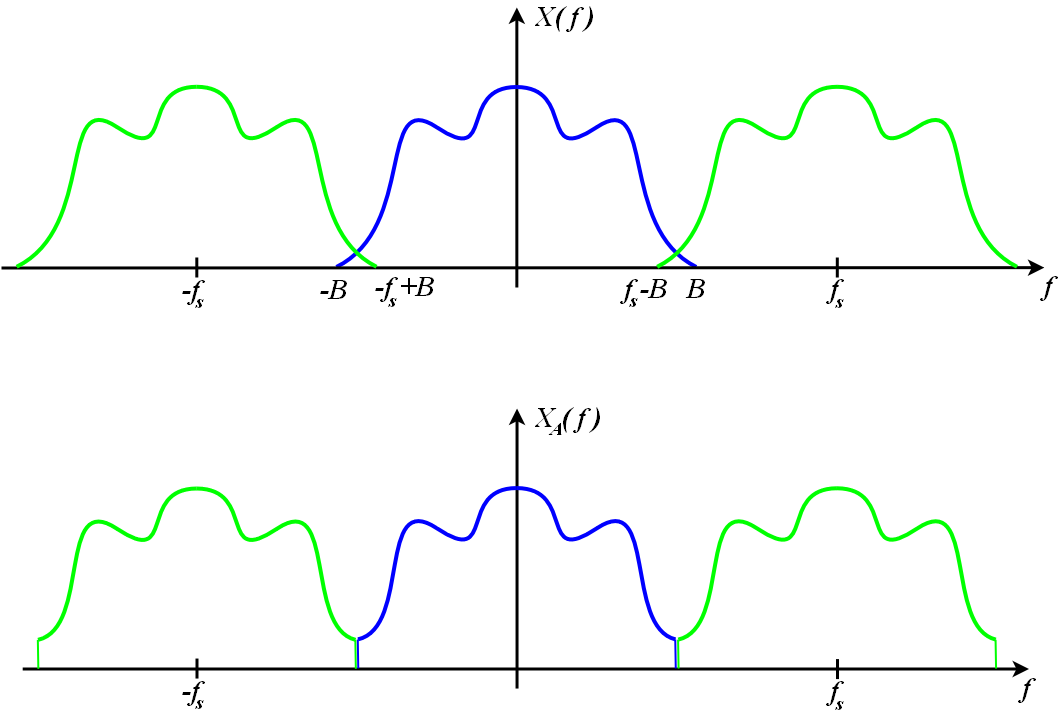
\includegraphics[width=1\textwidth]{EIRE2018Dateien/sonstige_Dateien/AliasedSpectrum}
		\centering
		\caption{
			Veranschaulichung des Effekts des Aliasing. Dargestellt ist ein Beispielsignal, das mit der Abtastfrequenz $f_S$ abgetastet wurde.
			Da diese geringer ist als das Doppelte der höchsten Frequenz im Signal $B$, überlappen sich die Perioden im Frequenzraum.
			Das ursprüngliche Signal kann durch einen Tiefpass nur unter Verlust der höheren Frequenzen rekonstruiert werden. \cite{Aliasing}
		}
		\label{fig_Aliasing_veranschaulichung}
		\centering
	\end{figure}
	
	
	%eig. zunächst Fertigstellung von Tag2 Teil 1
	\subsection{Leakage-Effekt und Fensterfunktion}
	\label{leakage}
	Wenn die Signalfrequenz kein Vielfaches des Produkts aus Abtastfrequenz und Zahl an Messpunkten pro Messung ist, tritt aufgrund der Endlichkeit des Messprozesses der sogenannte \enquote{Leakage-Effekt} auf.
	%https://de.wikipedia.org/wiki/Datei:Spectral_leakage_Sine.svg
	Dieser verursacht eine Verbreiterung des Peaks der Signalfrequenz im Frequenzbild.
	Dies ist in \cref{fig_leakage_veranschaulichung} dargestellt.
	
	\begin{figure}[H]  
		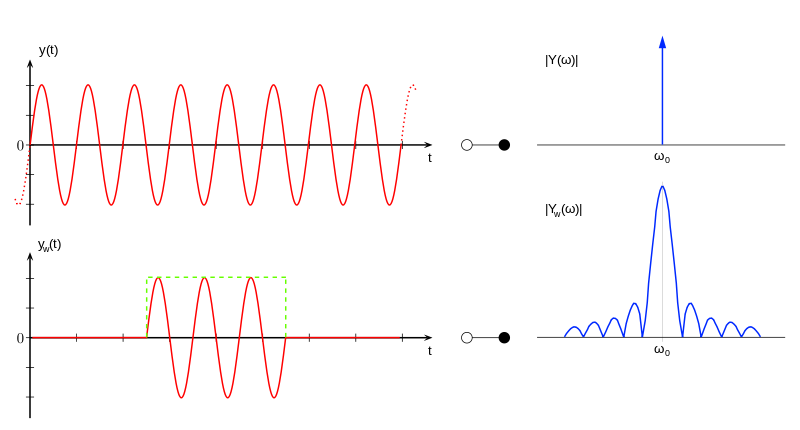
\includegraphics[width=1\textwidth]{EIRE2018Dateien/sonstige_Dateien/leakage}
		\centering
		\caption{
			Zeitlich nicht limitierte (\enquote{ungefensterte}) Sinusschwingung oben, zeitlich limitierte Sinusschwingung unten (limitiert mit Rechteck-Fensterfunktion) und daneben deren Fourier-Transformierten.\cite{Leakage}
		}
		\label{fig_leakage_veranschaulichung}
		\centering
	\end{figure}

	Um diesen Effekt zu minimieren kann das Signal mit einer Fensterfunktion multipliziert werden. % mit denen das Signal mutlipliziert wird? Wäre das immer wahr? - Jannik: Nach Wiki wird immer mit Fensterfunktion multipliziert: "Das Signal wird im Frequenzbereich mit diesem Spektrum der Fensterfunktion gefaltet(...)", https://de.m.wikipedia.org/wiki/Fensterfunktion#Beispiele_von_Fensterfunktionen
	Im Folgenden wird das \enquote{Von-Hann-Fenster} (auch \enquote{Hanning-Fenster}) verwendet, welches der Haversine-Funktion entspricht ($\frac{1-\cos \vartheta}{2} $). %mehr erklären? Hat er halt auch nicht so schöne gemacht, nur halt 1-cos - Jannik: Wenn du oben sagst, dass man das Signal mit der Fensterfunktion multipliziert, kannst du hier ganz kurz sagen, dass die Fensterfunktion des Von-Hann-Fensters die Haversine-Funktion ist (https://de.m.wikipedia.org/wiki/Fensterfunktion#Von-Hann-Fenster). Damit sollte man so mehr oder weniger wissen was gemeint ist. >> Würde ich nicht erwähnen, da es genauso klar wie nur von Hann ist und ich mir mit Wiki nicht sicher bin, ob Haversine nicht nur ein Spezialfall des von-Hann-Fensters ist.
	Der Unterschied zwischen Spektralanalyse mit und ohne Von-Hann-Fenster ist in \cref{fig_tag23_oszi_manuell_front} zu erkennen, da dort ohne Fenster-Funktion zusätzliche Frequenzen in der Nähe des Peaks auftreten.
	

	\subsection{Digitales Oszilloskop ohne ExpressVI} % hier ist halt die Tagreihenfolge bissl gebrochen. Ich glaube, wir haben das an Tag 2 angefangen und Tag 3 beendet
	Das Oszilloskopprogramm von zuvor wird ersetzt durch eines, das anstelle des ExpressVIs Konfiguration, Messung und Cleanup getrennt enthält.
	Dieses ist in \cref{fig_tag23_oszi_manuell_block} dargestellt, während in \cref{fig_tag23_oszi_manuell_front} die Frontplatte bei einem Eingangssignal von \SI{600}{\hertz} abgebildet ist.
	
	\begin{figure}[H]  
		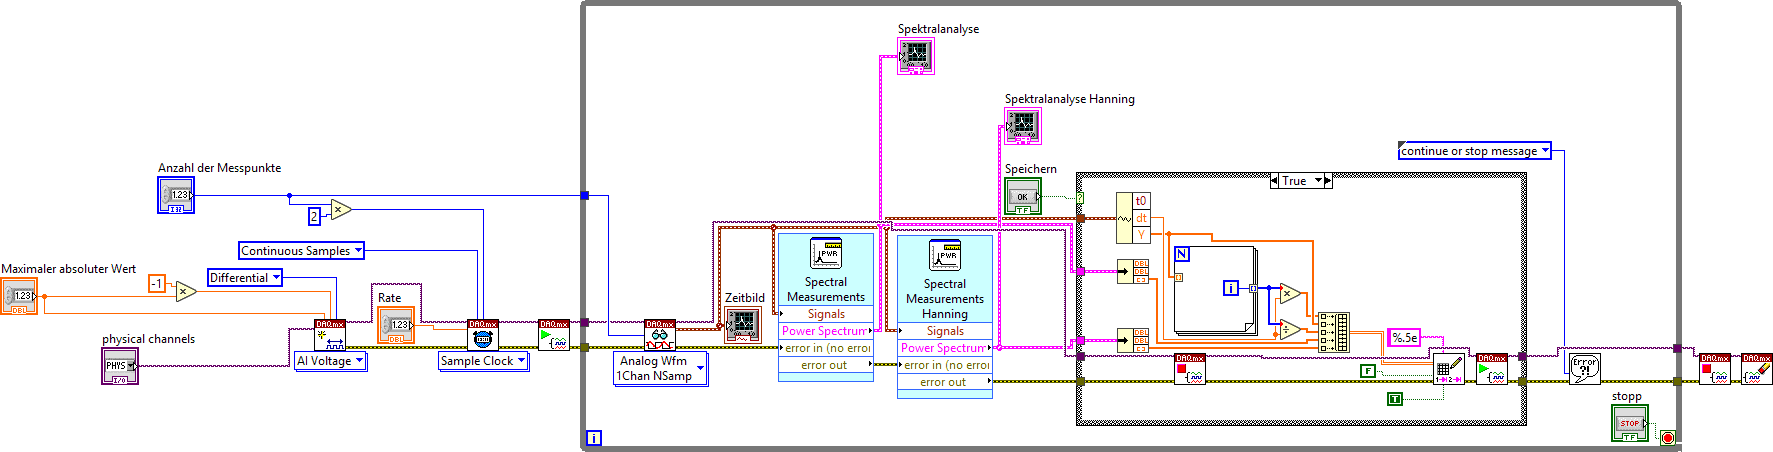
\includegraphics[width=1\textwidth]{EIRE2018Dateien/Tag3/ManuellVId}
		\centering
		\caption{
			Oszilloskopprogramm, das eine Abtastung vornimmt und das Ergebnis im Zeitbild sowie im Frequenzbild mit und ohne Hann-Fenster darstellt.
			Außerdem ist die Speicherung der Daten in einem Textdokument ermöglicht.
		}
		\label{fig_tag23_oszi_manuell_block}
		\centering
	\end{figure}

	\begin{figure}[H]  
		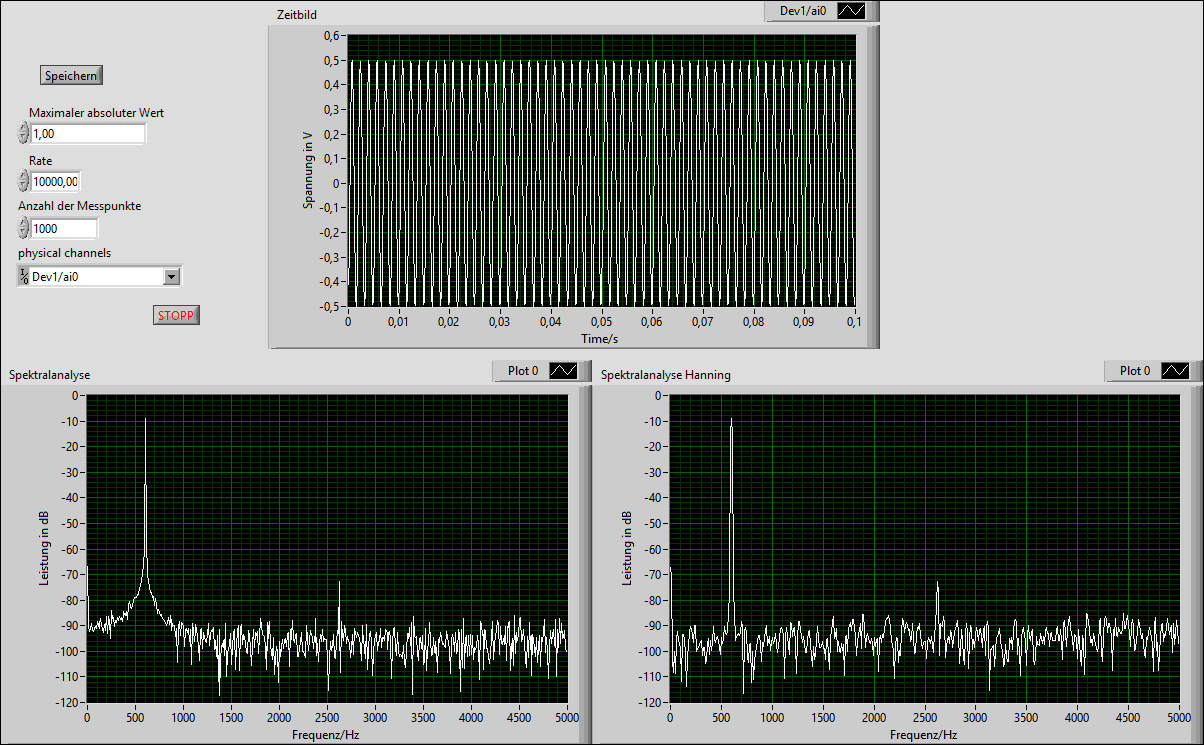
\includegraphics[width=1\textwidth]{EIRE2018Dateien/Tag3/ManuellVIp}
		\centering
		\caption{
			Oszilloskopfrontplatte. Dargestellt wird das gemessene Signal im Zeitbild sowie im Frequenzbild mit und ohne Von-Hann-Fenster. Einstellbar ist die Abtastfrequenz, die Anzahl der Messpunkte, der Eingangskanal des Messgerätes und der maximale messbare Wert, wobei der minimale auf das Negative des maximalen gesetzt wird.
			Mithilfe des Stopp-Knopfes kann das Programm gestoppt werden und mit dem Speichern-Knopf werden die aktuellen Messwerte aus allen drei Diagrammen in eine Textdatei exportiert.
		}
		\label{fig_tag23_oszi_manuell_front}
		\centering
	\end{figure}

	Hierbei wird ebenfalls die Möglichkeit die aktuellen Messwerte zu speichern eingeführt.
	Dazu werden die Strukturen aus verschiedenen Datentypen, die in den Diagrammen dargestellt werden, in ihre Bestandteile zerlegt und die Arrays der Y-Werte mit zwei Arrays für fortlaufende Zeit- und Frequenzwerte kombiniert und der Speicherfunktion zugeführt.
	Der Speichervorgang befindet sich innerhalb eines case-Konstrukts, das ignoriert wird, solange der Speichern-Knopf nicht gedrückt wurde.
	Außerdem werden Fehlermeldungen einer Fehlerdialogfunktion zugeführt, die dem Nutzer erlaubt bei Fehlern wahlweise das Programm anzuhalten oder weiterlaufen zu lassen.
	Um ein Volllaufen des Mess-Buffers zu vermeiden, wird dieser doppelt so groß wie die Anzahl der Messpunkte pro Zyklus gewählt.
	\subsection{Aliasing}
	Um den Effekt des Aliasings absichtlich herbeizuführen, werden bei einer Abtastfrequenz von \SI{1000}{\hertz} zwei verschiedene Signale abgetastet.
	Da bei dieser Abtastfrequenz die höchste Frequenz im Signal kleiner als \SI{500}{\hertz} sein muss, ist hierbei zu erwarten, dass ein Signal von \SI{400}{\hertz} korrekt abgetastet wird, während eines mit \SI{600}{\hertz} falsch abgetastet wird.
	Das Spektrum des abgetasteten Signals bei diesen beiden Signalfrequenzen ist in \cref{fig_ali} dargestellt.
	
	\begin{figure}[H]
		\centering
		\begin{subfigure}[t]{0.5\textwidth}
			\centering
			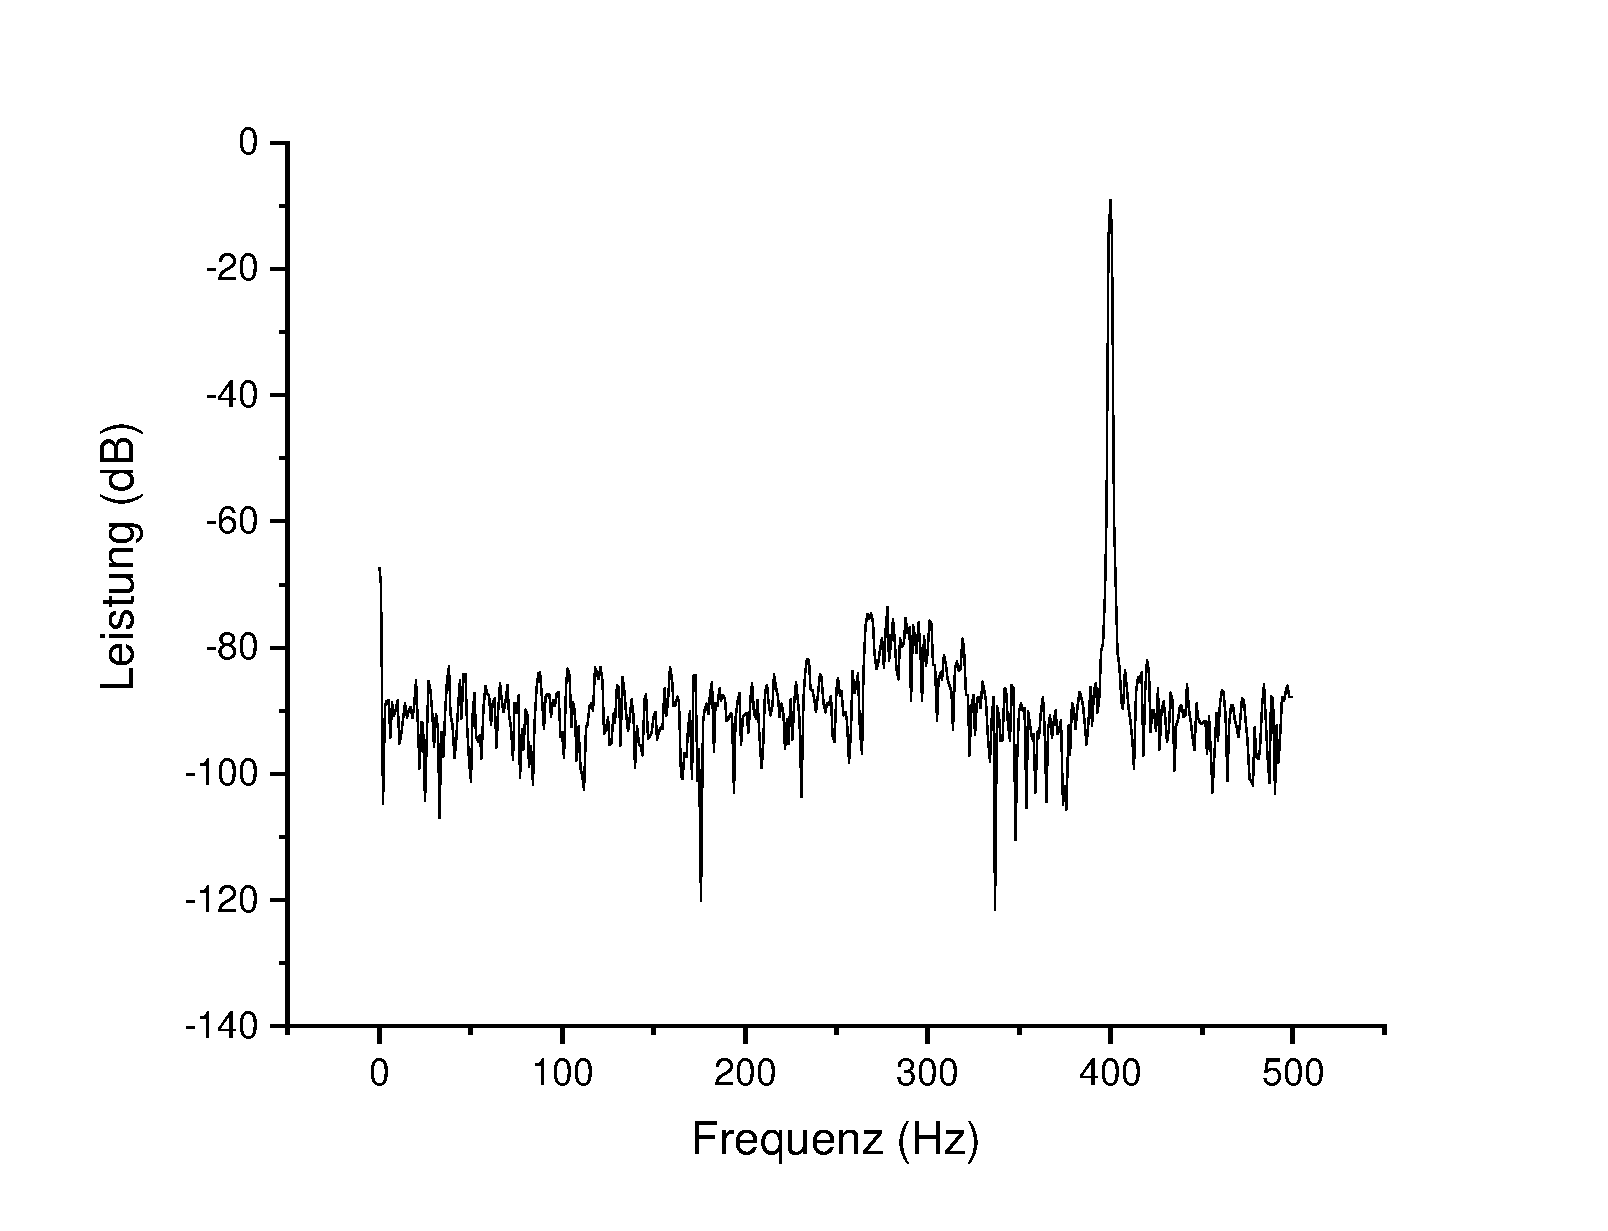
\includegraphics[width=1\textwidth]{Origin-Files/aliasing_abtast1000bei400sig}
			\caption{\SI{400}{\hertz}}
		\end{subfigure}%
		\begin{subfigure}[t]{0.5\textwidth}
			\centering
			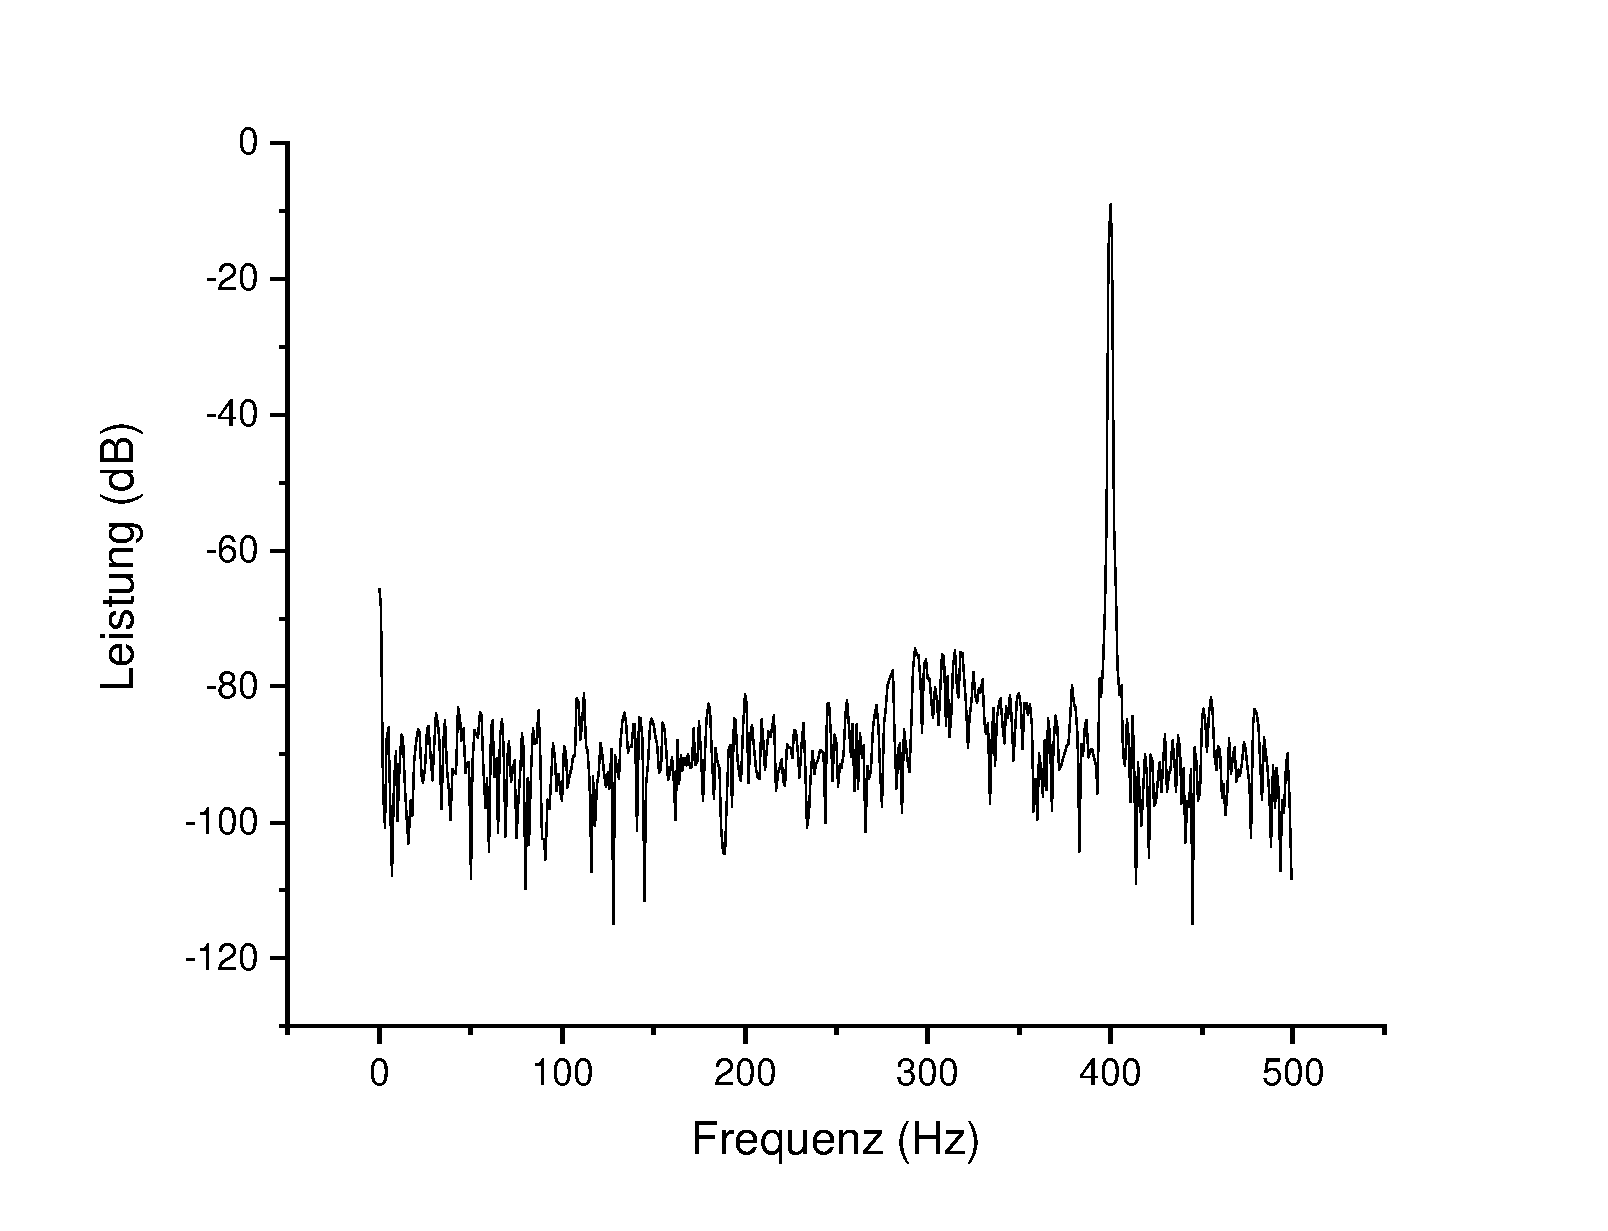
\includegraphics[width=1\textwidth]{Origin-Files/aliasing_abtast1000bei600sig}
			\caption{\SI{600}{\hertz}}
		\end{subfigure}
		
		\caption{Mit einer Abtastfrequenz von \SI{1000}{\hertz} abgetastete Signale, deren Frequenz einmal \SI{400}{\hertz} und einmal \SI{600}{\hertz} beträgt, sodass einmal korrekt und einmal falsch abgetastet wird. Um die Sichtbarkeit zu verbessern und die übliche Oszilloskop-Optik zu erreichen, wurden die Messpunkte hier und in den folgenden Darstellungen mit einer Linie verbunden.} %mir gefällt nicht ganz, dass das in einer caption steht, aber überall sonst wäre auch nicht optimal von daher frack it
		\label{fig_ali}
		\centering
	\end{figure}
	
	Es fällt auf, dass sich zwischen diesen beiden Signalen kein Unterschied erkennen lässt.
	Dies liegt daran, dass bei einer Signalfrequenz von \SI{600}{\hertz} die eigentliche Signalfrequenz nicht mehr vom idealen Tiefpass übertragen wird, während die Differenzfrequenz von Abtastfrequenz und Signalfrequenz \SI{400}{\hertz} beträgt und noch übertragen wird.
	Es ist an den beiden Signalen zu erkennen, dass sich ein falsch abgetastetes Signal nicht mehr von einem korrekt abgetasteten Signal bei der entsprechenden Differenzfrequenz unterscheiden lässt.
	Man stellt fest, dass man vor der Abtastung bereits wissen muss, welche Frequenzen im Signal vorkommen. 
	
	\subsection{Unpassende Abtastrate}
	Um den Leakage-Effekt, der in \cref{leakage} beschrieben wurde, zu bebildern, wird er in \crefrange{fig_tag3_unpassend_230hz}{fig_tag3_unpassend_235hz} absichtlich herbeigeführt.
	Dabei wird hier das Produkt aus Abtastfrequenz und Anzahl der Messpunkte pro Messdurchgang als \enquote{Abtastrate} bezeichnet. %Anführungsstriche gut?
	Hier beträgt die Abtastfrequenz \SI{1000}{\hertz} und die Anzahl der Messpunkte pro Messdurchgang \num{100}, woraus sich eine Abtastrate von \SI{10}{\hertz} ergibt.
	Wenn die Signalfrequenz kein Vielfaches der Abtastrate ist, führt dies dazu, dass eine eigentlich scharfe Frequenz im Spektrum unscharf wird und Frequenzen geringerer Intensität in der Nähe dieser überdeckt werden.
	Man stellt fest, dass man, wenn man die Signalfrequenz kennt, die Abtastrate richtig wählen muss und sich, wenn dem nicht so ist, die Verwendung einer Fensterfunktion empfiehlt.
	%mir ist erst spät klar geworden, dass das der fenster-Kram ist.
	%kp, ob ich hier auch die gefensterten reintun sollte, denke nicht
	
	\begin{figure}[H]  
		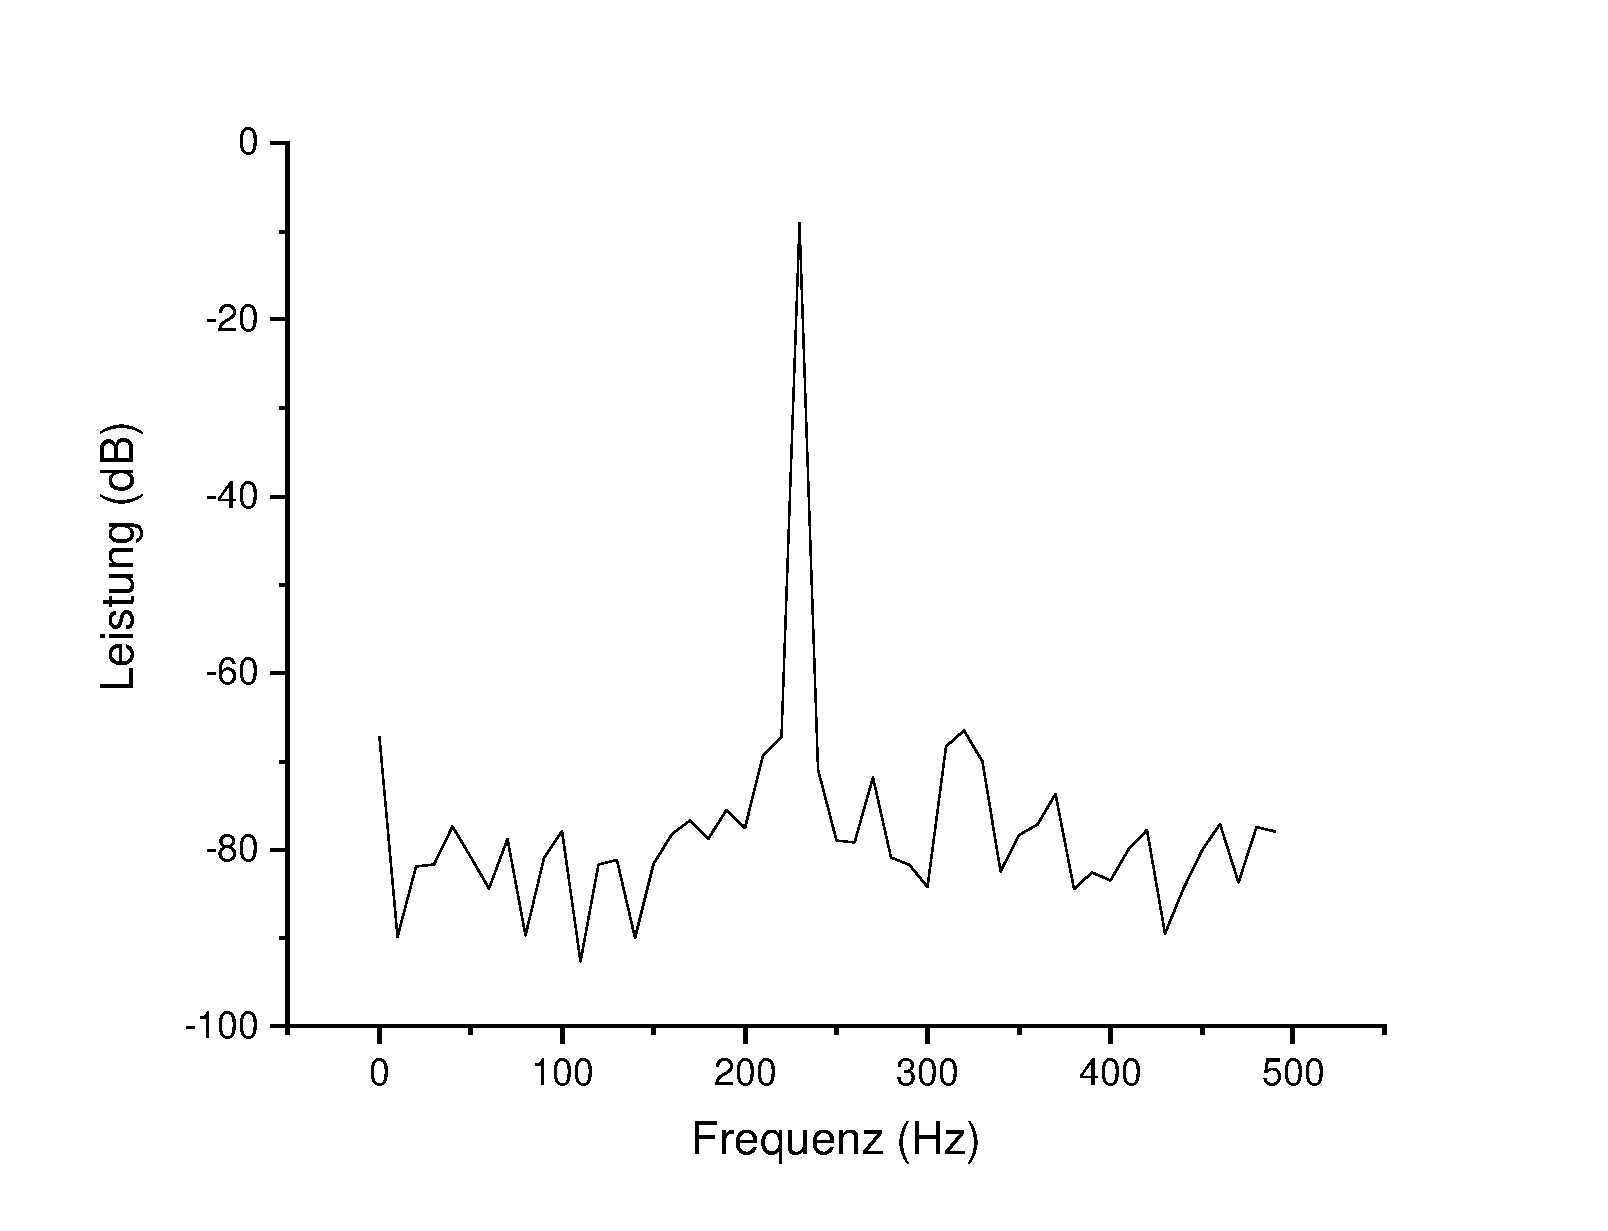
\includegraphics[width=0.5\textwidth]{Origin-Files/unpassend_230nonhann}
		\centering
		\caption{
			Spektrum eines Signals mit einer Frequenz von \SI{230}{\hertz}, was ein Vielfaches der Abtastrate ist, weshalb hier die Signalfrequenz scharf zu erkennen ist. Eine Fensterfunktion wurde hier nicht verwendet.
		}
		\label{fig_tag3_unpassend_230hz}
		\centering
	\end{figure}
	
	\begin{figure}[H]  
		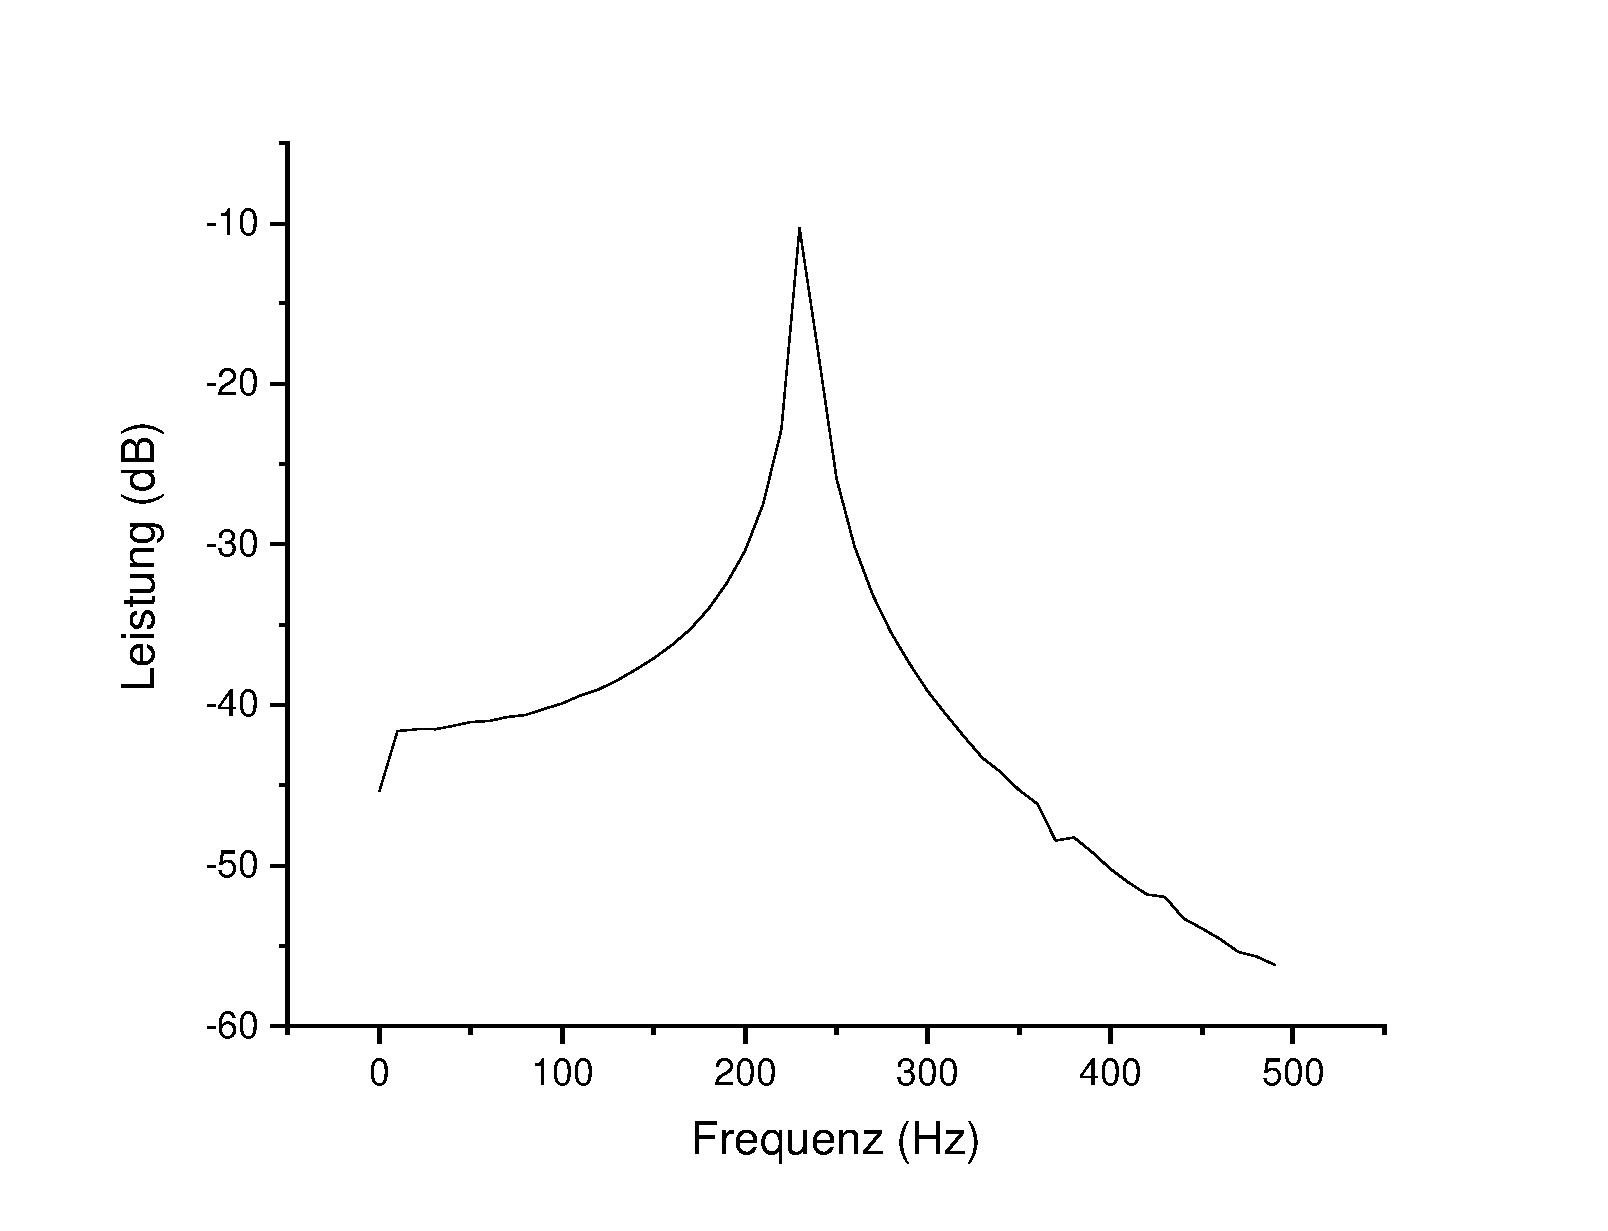
\includegraphics[width=0.5\textwidth]{Origin-Files/unpassend_233nonhann}
		\centering
		\caption{
			Spektrum eines Signals mit einer Frequenz von \SI{233}{\hertz}, was kein Vielfaches der Abtastrate ist, weshalb hier zu erkennen ist, dass die Signalfrequenz unscharf wird. Eine Fensterfunktion wurde hier nicht verwendet.
		}
		\label{fig_tag3_unpassend_233hz}
		\centering
	\end{figure}
	
	\begin{figure}[H]  
		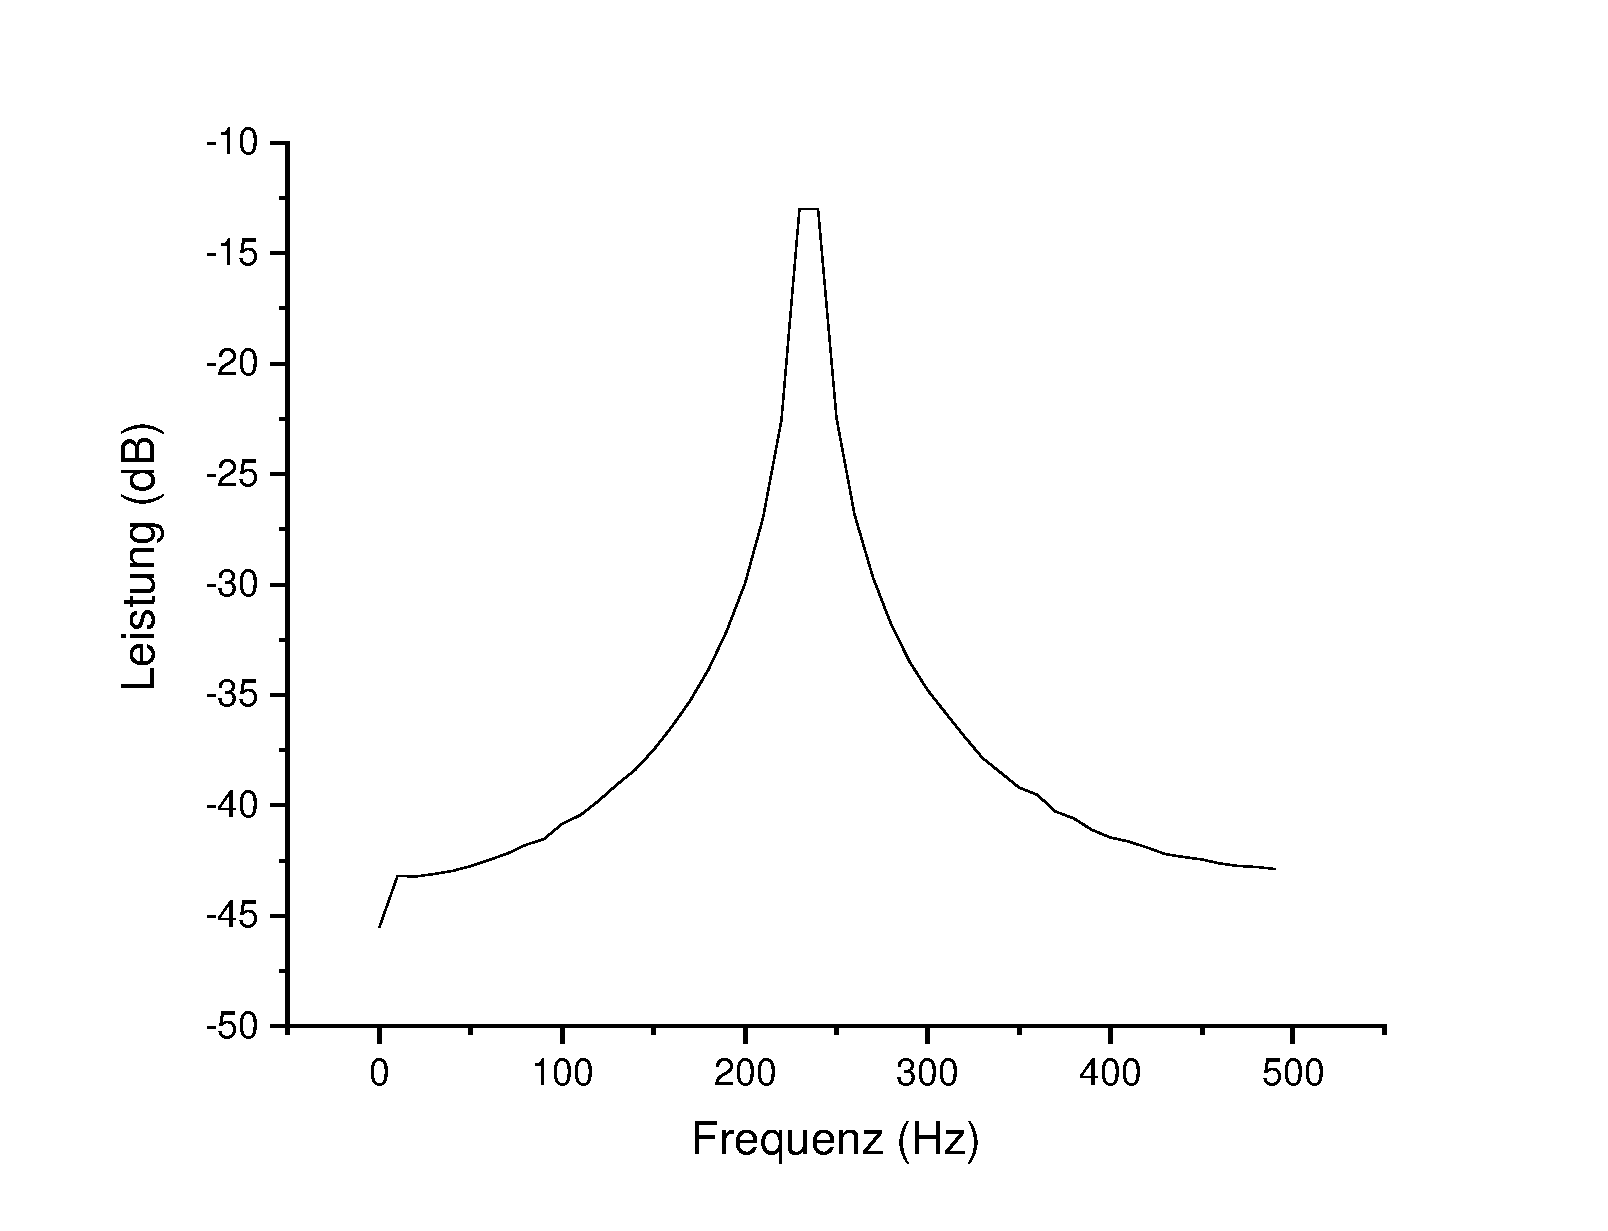
\includegraphics[width=0.5\textwidth]{Origin-Files/unpassend_235nonhann}
		\centering
		\caption{
			Spektrum eines Signals mit einer Frequenz von \SI{235}{\hertz}, was kein Vielfaches der Abtastrate ist, weshalb hier zu erkennen ist, dass die Signalfrequenz unscharf wird. Eine Fensterfunktion wurde hier nicht verwendet.
		}
		\label{fig_tag3_unpassend_235hz}
		\centering
	\end{figure}
	
	\newpage
	
	
	\section{Amplitudenmodulierte Signale}

	\subsection{Erzeugung eines amplitudenmodulierten Signals} \label{AMSignalErzeugung}
	
	Es soll nun ein amplitudenmoduliertes Signal (auch als AM-Signal bezeichnet) erzeugt werden und über die Soundkarte des verwendeten PCs ausgegeben werden.
	Dann wird das Signal der Soundkarte wieder auf den Analog-Digital-Wandler gegeben und mit dem zuvor erstellten Oszilloskopprogramm verarbeitet.
	In \cref{fig_tag3_am_soundkarte_block} ist das dazu verwendete LabView-Programm dargestellt.
	Moduliert werden soll die Überlagerung zweier Signale mit einstellbarer Frequenz und Amplitude.
	Auch Trägerfrequenz und Modulationsgrad soll einstellbar sein.
	Die Amplitudenmodulation lässt sich durch die Gleichung
	
	\begin{equation} \label{AMFormel}
		S_{AM}(t)=S_T (1+m \cdot s(t)) \cdot \cos(2\pi f_T t)
	\end{equation}
	
	\noindent beschreiben.
	Dabei ist $m$ der Modulationsgrad, $f_T$ die Trägerfrequenz und $S_T$ die Amplitude.
	Da die Überlagerung von zwei sinusförmigen Signalen beliebiger aber fester Frequenz moduliert werden soll gilt:
	
	\begin{equation} \label{Ursprungssignal}
		s(t) = A_1 \cos (2\pi f_1 t) + A_2 \cos (2\pi f_2 t) \ . 
	\end{equation}
	
	\noindent Dabei sind $A_1$ und $A_2$ die Amplituden und $f_1$ und $f_2$ die Frequenzen der Signale.
	
	Diese beiden Gleichungen sollen im Folgenden durch Operationen auf Arrays realisiert und als Audiosignal ausgegeben werden.	
	Dazu wird das in \cref{sinusfkt} erstellte Programm verwendet, um Arrays von Sinusfunktionen zu erstellen.
	Diesem wird in jedem Fall die Phase $0$ zugeführt und es werden $44100$ Stützstellen gewählt, weil dies der Abtastrate bei CDs entspricht.
	Dem Programm wird zunächst eine Amplitude von $1$ gegeben und dann werden alle Array-Elemente mit der gewählten Amplitude multipliziert.
	Dies hängt lediglich damit zusammen, dass zuvor im Sinus-erstellenden Programm ein Fehler vorhanden war, der dies nötig machte (vgl. \cref{sinus_amp_fehler}).
	In \cref{fig_tag3_am_soundkarte_block} ist zu erkennen, dass zunächst zwei Sinus-Arrays erstellt werden, für die jeweils eine Signalfrequenz und -amplitude gewählt werden.
	Die beiden resultierenden Arrays werden addiert, mit dem Modulationsgrad multipliziert und dann mit dem Array der Trägerfrequenz multipliziert.
	Dieses wurde zuvor in gleicher Art und Weise mit dem Sinus-Programm bei der einstellbaren Trägerfrequenz erstellt.
	Für die Amplitude des Trägersignals wird der Kehrwert der maximalen Signalamplitude gewählt, damit die resultierende Amplitude immer auf $1$ liegt, da die Soundkarte höhere Werte nicht verarbeitet.
	Das resultierende Array wird im Zeit- und Frequenzbild dargestellt und dann mithilfe der entsprechenden VIs über die Soundkarte ausgegeben.
	Hierfür wird die Abtastrate auf \SI{44100}{\hertz}, die Anzahl der Kanäle auf $1$ eingestellt und der Modus \enquote{Continuos Samples} gewählt, da das Signal fortlaufend erzeugt werden soll.
	Außerdem wird das Element zur Ausgabe von Fehlern verwendet, das es erlaubt das Programm beim Auftreten von Fehlern wahlweise zu beenden oder weiterlaufen zu lassen. %ich wollte hier noch was mit "das Signal in jedem Schleifendurchlauf" schreiben, aber ich weiß nicht mehr was
	
	\begin{figure}[H]  
		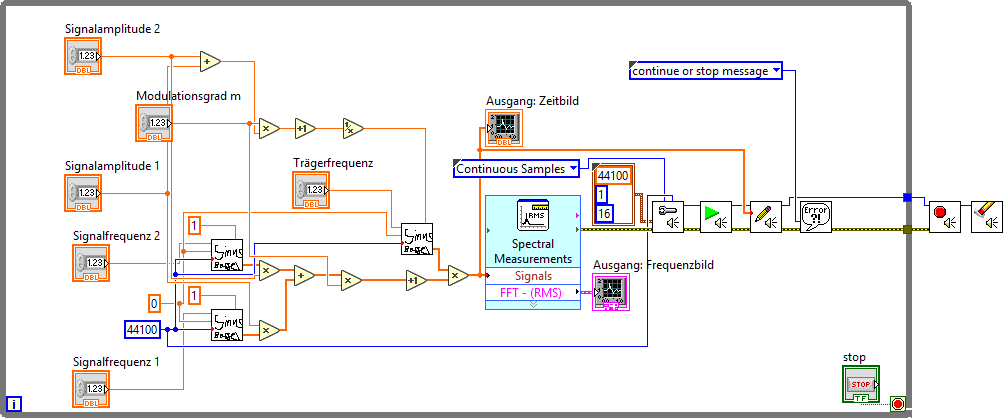
\includegraphics[width=1\textwidth]{EIRE2018Dateien/Tag3/Soundkarteoutoszi/AMd}
		\centering
		\caption{
			Blockdiagramm des Programms zur Erzeugung eines amplitudenmodulierten Signals und Ausgabe dessen über die Soundkarte.
		}
		\label{fig_tag3_am_soundkarte_block}
		\centering
	\end{figure}
	
	\begin{figure}[H]  
		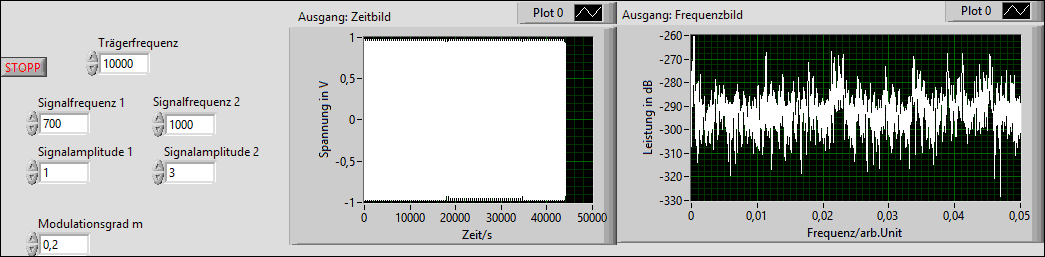
\includegraphics[width=1\textwidth]{EIRE2018Dateien/Tag3/Soundkarteoutoszi/AMp}
		\centering
		\caption{
			Frontplatte des Programms zur Erzeugung eines amplitudenmodulierten Signals und Ausgabe dessen über die Soundkarte.
		}
		\label{fig_tag3_am_soundkarte_front}
		\centering
	\end{figure}

	
\iffalse %auskommentiert weil ergibt keinen Sinn und ist eh später zu sehen.
	\begin{figure}[H]
		\centering
		\begin{subfigure}[t]{0.5\textwidth}
			\centering
			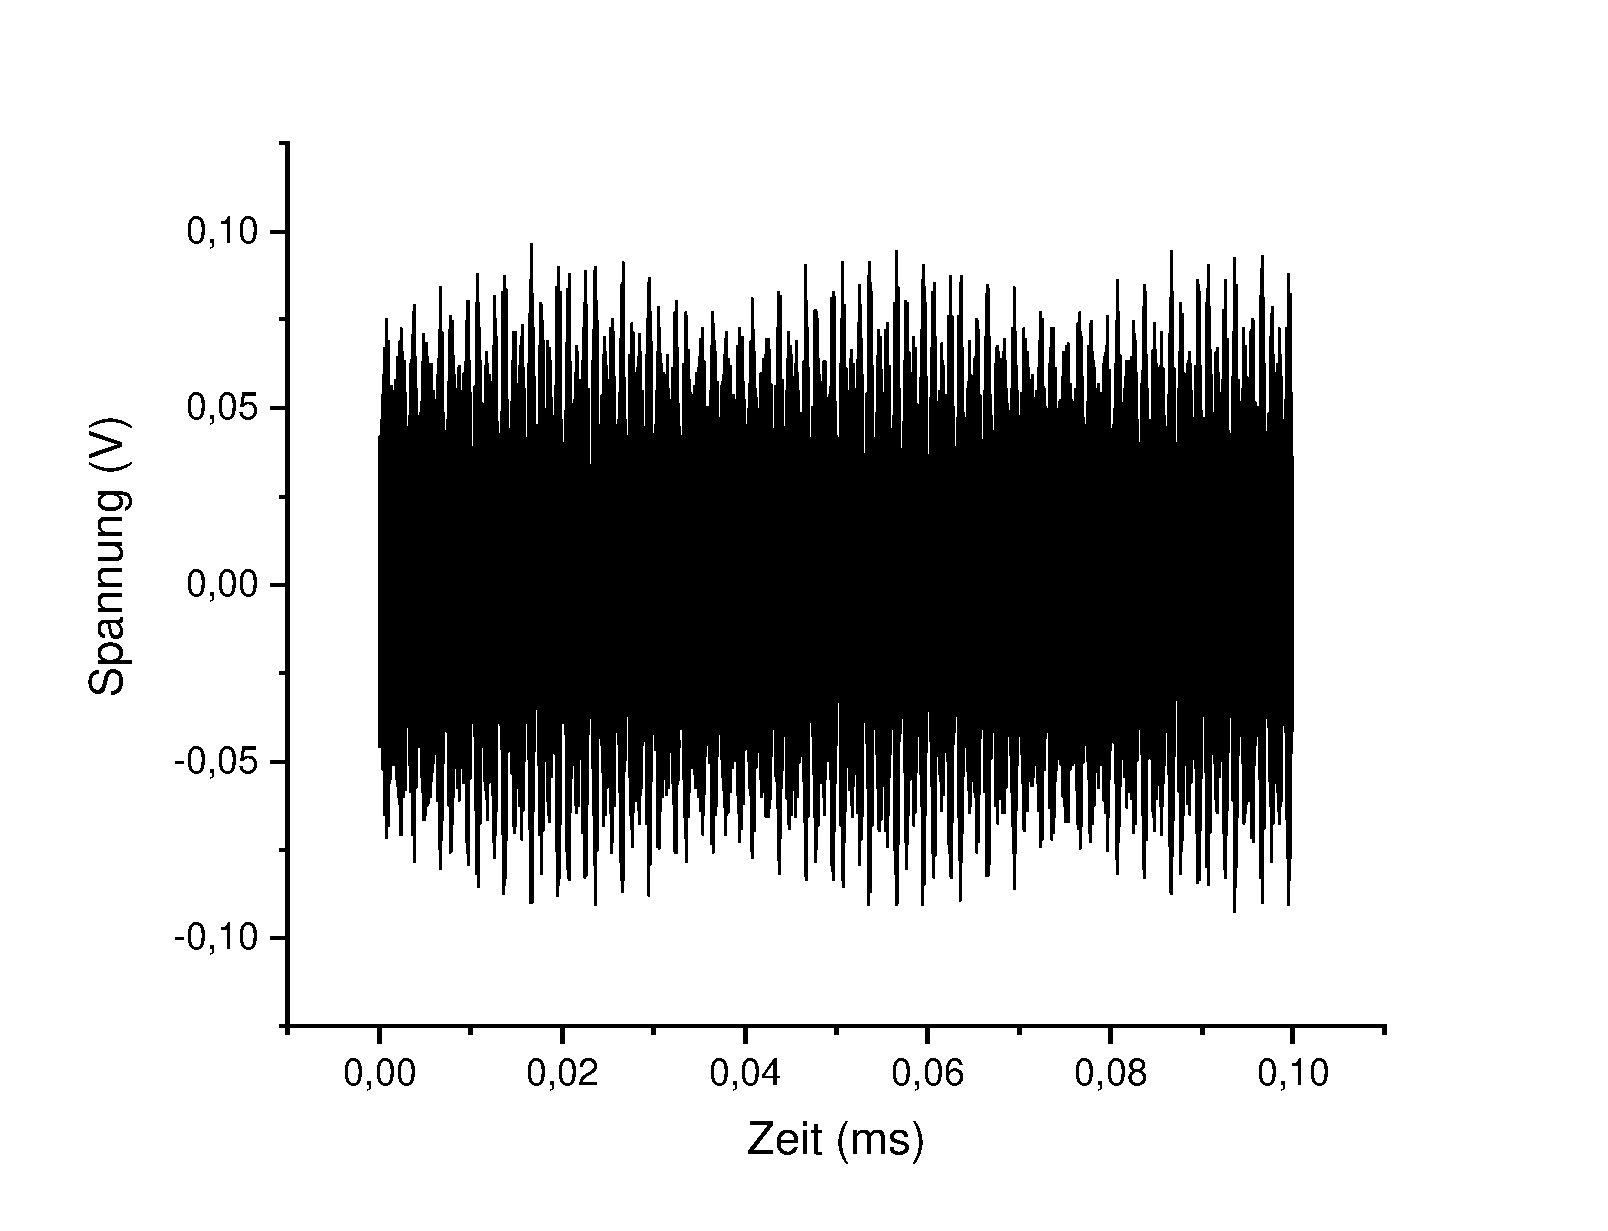
\includegraphics[width=1\textwidth]{Origin-Files/AM-Zeit}
			\caption{Zeitdomäne}
		\end{subfigure}%
		\begin{subfigure}[t]{0.5\textwidth}
			\centering
			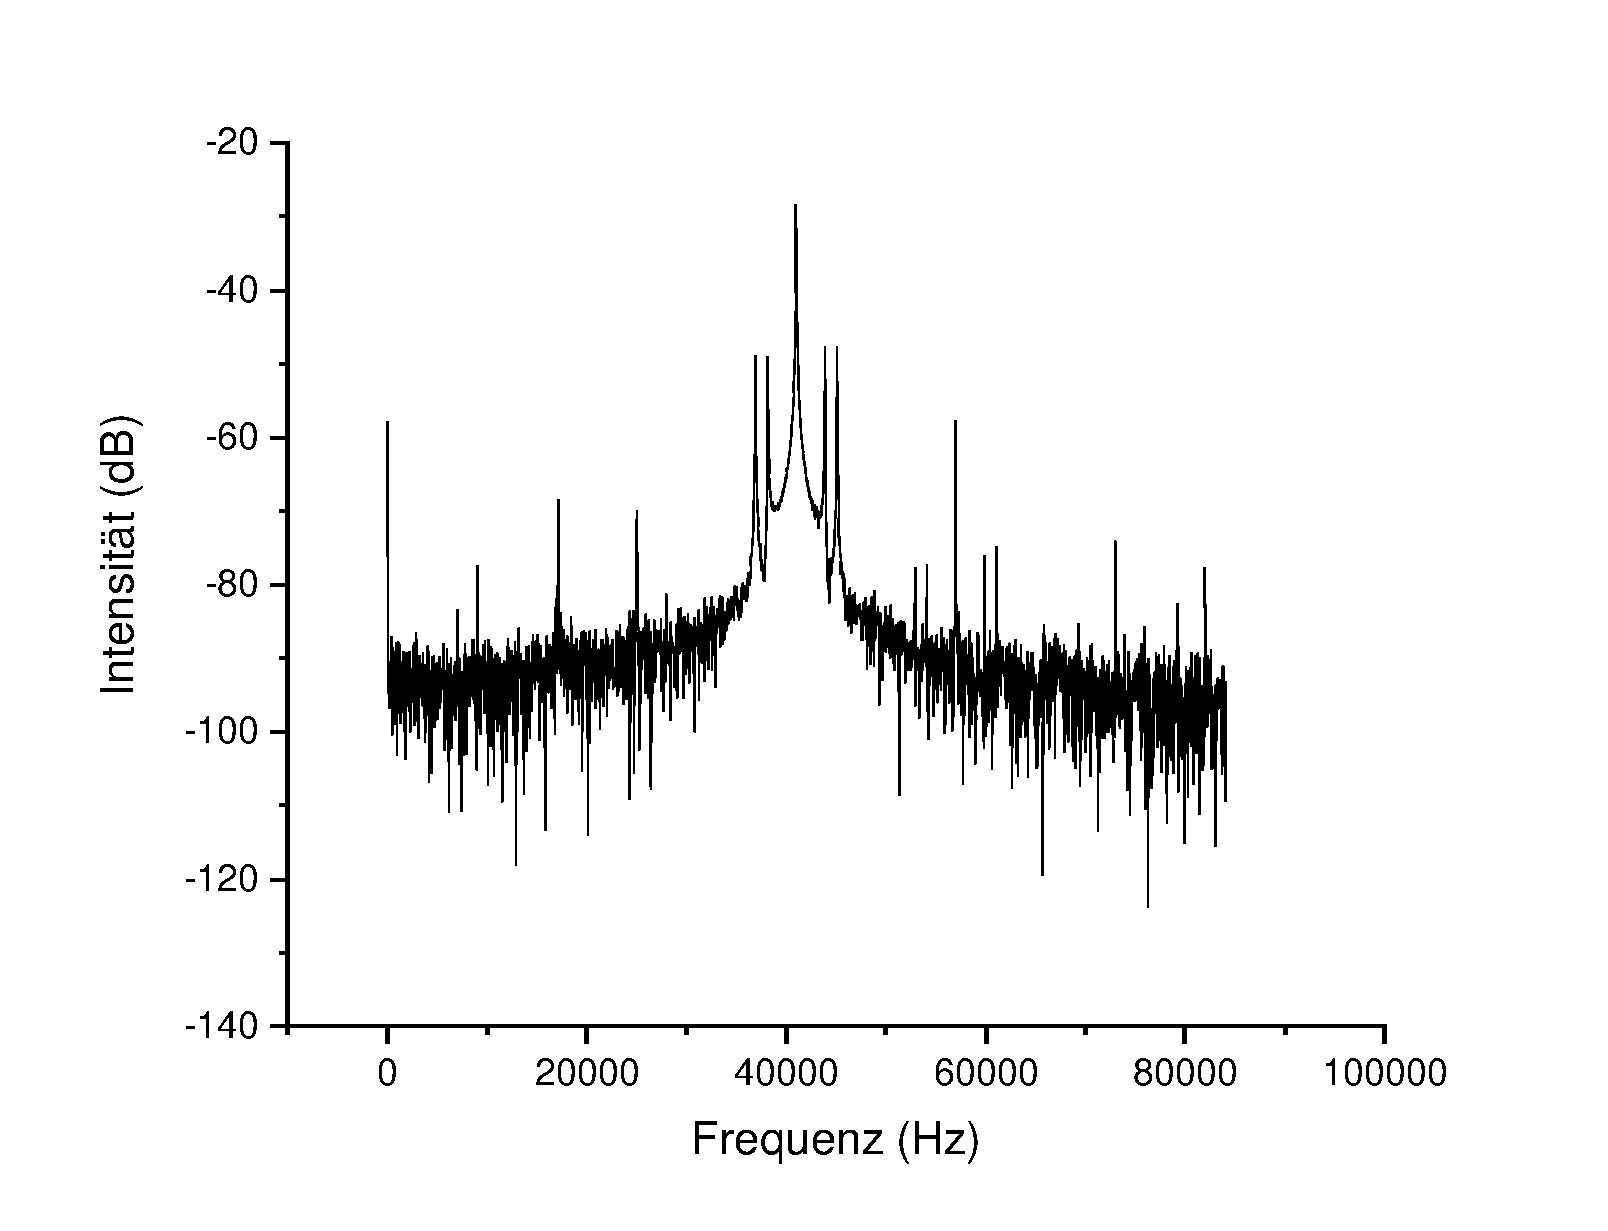
\includegraphics[width=1\textwidth]{Origin-Files/AM-Freq-Hann}
			\caption{Frequenzdomäne}
		\end{subfigure}
		\label{fig_tag3_am_soundkarte}
		\caption{Ausgabe des Oszilloskopprogramms in der Zeit- und Frequenzdomäne bei Erfassung des amplitudenmodulierten Signals, das mittels der Soundkarte ausgegeben wird.}
		\centering
	\end{figure}
\fi

	Auf das Ergebnis der Modulation wird im folgenden Abschnitt eingegangen.
	
	%Rausgenommen, weil komisch und nicht wichtig:
	%In der Frequenzdomäne lässt sich hier erkennen, dass die eingestellte Trägerfrequenz von %TODO hart komisch
	%Darüber hinaus ist zu sehen, dass einige zusätzliche Frequenzen erheblicher Leistung auftreten.
	%Diese lassen sich nur durch Störeffekte bei der Erzeugung des Signals durch die Soundkarte erklären. %und theoretisch durch Erfassung, halte ich halt für unwahrscheinlicher
	
	\subsection{Demodulation eines AM-Signals durch Quadrieren und Betragsbildung} \label{DemodulationAM}
	%Betrag, Quadrat
	Um nun das amplitudenmodulierte Signal im Oszilloskopprogramm wieder demodulieren zu können, wird ein Case-Konstrukt eingeführt, welches nach Auswahl des Benutzers entweder das Signal nicht demoduliert, mit sich selbst multipliziert oder den Betrag des Signals bildet, da in den letzten beiden Fällen unter anderem wieder die Ursprungsfrequenzen vorliegen.
	Nach diesem Schritt wird das Signal im Zeit- und Frequenzbild dargestellt und danach zusätzlich durch einen Tiefpass geführt, der auftretende höhere Frequenzen herausfiltert, und dann erneut im Zeit- und Frequenzbild dargestellt.
	Außerdem wird die Speicherung von zuvor erweitert, sodass das Signal vor der Demodulation, vor dem Tiefpass und nach diesem gespeichert werden kann.
	Das fertige Programm ist in \cref{fig_tag3_am_demod_block} und die zugehörige Frontplatte in \cref{fig_tag3_am_demod_front} dargestellt.
	Dass man in der Zeitdomäne letzterer wenig erkennen kann, liegt an der Vielzahl und der Größe der auftretenden Frequenzen.
	Diese Tatsache gilt für alle der kommenden Untersuchungen, weshalb im Folgenden nur noch die Frequenzdomäne dargestellt wird.
	

	\begin{figure}[H]  
		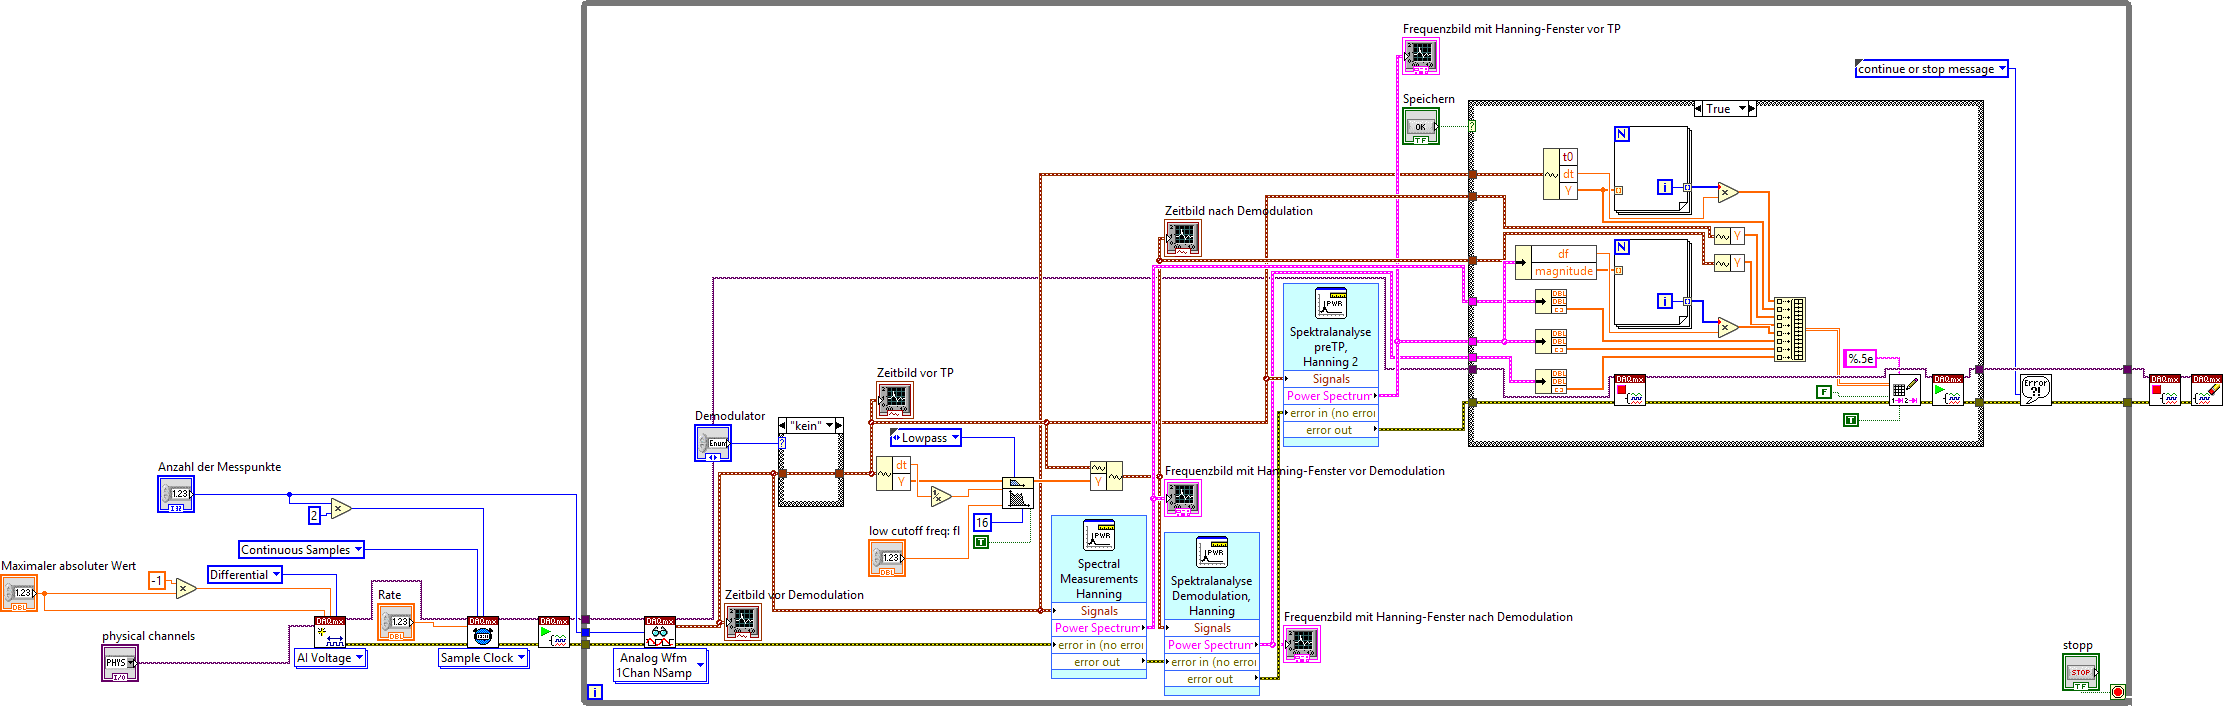
\includegraphics[width=1\textwidth]{EIRE2018Dateien/Tag3/modifizierterOszi/Oszilloskop__modifiziertd}
		\centering
		\caption{
			Blockdiagramm des Programms zur Demodulation und Darstellung eines amplitudenmodulierten Signals. Zur Demodulation kann Quadrieren und Bildung des Betrags gewählt werden. In diesen Fällen steht im Case-Konstrukt ein Quadrierer bzw. ein Multiplizierer.
		}
		\label{fig_tag3_am_demod_block}
		\centering
	\end{figure}

	\begin{figure}[H]  
		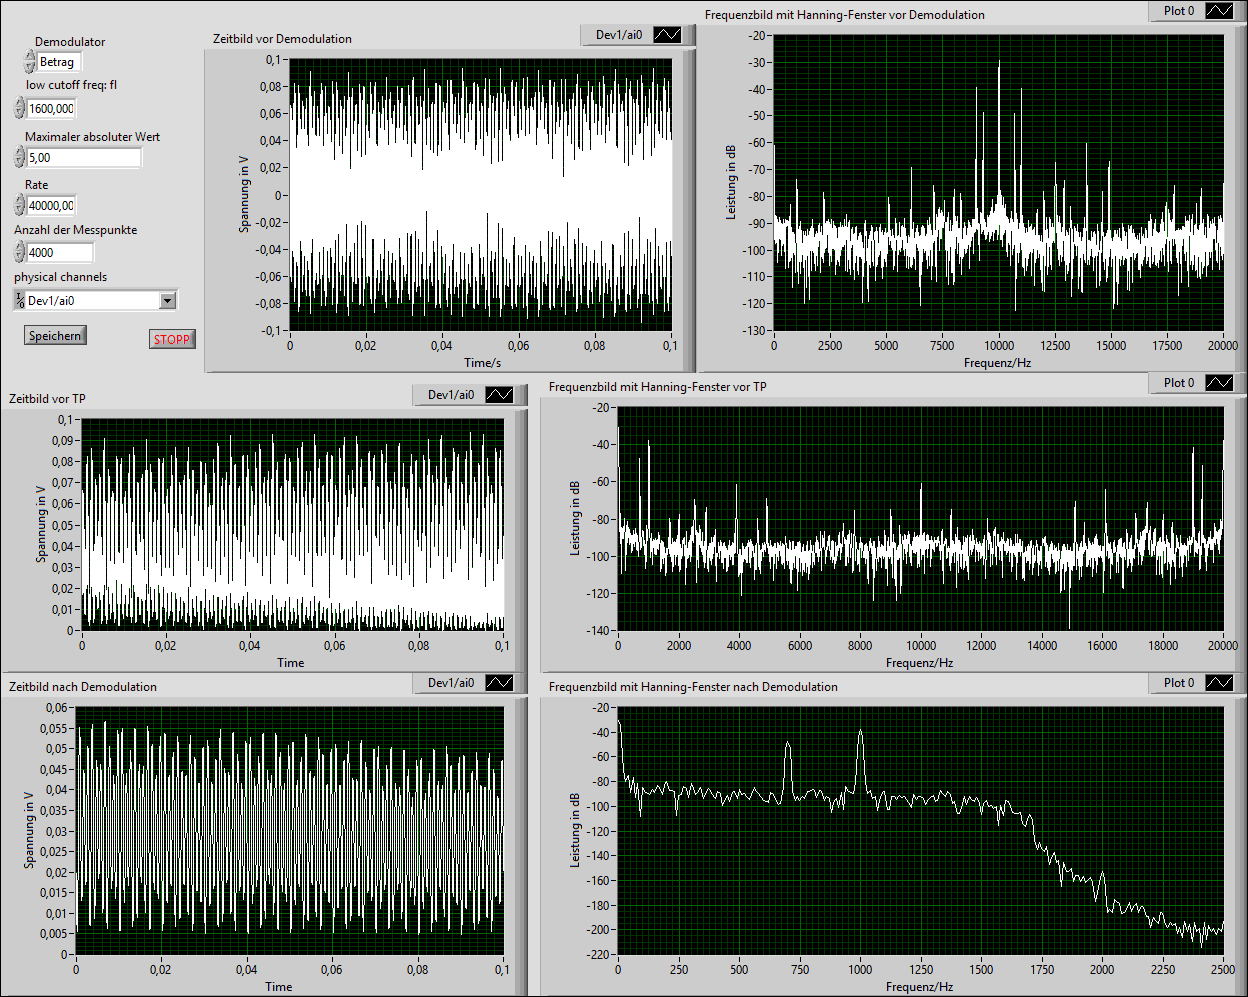
\includegraphics[width=0.7\textwidth]{EIRE2018Dateien/Tag3/modifizierterOszi/Oszilloskop__modifiziertp}
		\centering
		\caption{
			Frontplatte des Programms zur Demodulation und Darstellung eines amplitudenmodulierten Signals.
			Einstellbar ist die Art der Demodulation (keine, Quadrieren, Betragsbildung), die Grenzfrequenz des Tiefpasses nach der Demodulation, maximal messbarer Wert, Messfrequenz, Anzahl der Messpunkte pro Messdurchgang und Eingangskanal, an dem der Analog-Digital-Wandler angeschlossen ist.
			Die Grafiken zeigen jeweils im Zeit- und Frequenzbild (mit Hanning-Fensterfunktion) das Signal vor, nach und während der Demodulation.
			Die aktuellen Punkte in allen sechs Grafiken können in einer Textdatei gespeichert werden.
		}
		\label{fig_tag3_am_demod_front}
		\centering
	\end{figure}

	In \crefrange{fig_tag3_am_demod_eingang}{fig_tag3_am_demod_quadrat_vollst} sind die Graphen, die sich aus der durch den \enquote{Speichern}-Knopf erstellten Textdatei ergeben, dargestellt.
	All diesen ist gemein, dass neben den rechnerisch durch die Modulation entstehenden Frequenzen noch einige andere von signifikanter Stärke vorhanden sind.
	Diese müssen auf Störeffekte durch Netzfrequenz, deren Oberfrequenzen und andere Effekte bei der Erzeugung durch die Soundkarte zurückgeführt werden.
	Im Folgenden wird immer ein amplitudenmoduliertes Signal mit einer Trägerfrequenz von \SI{10000}{\hertz} verwendet.
	Vor der Modulation beinhaltet das Signal die Frequenz \SI{700}{\hertz} mit einer relativen Amplitude von \num{1} und die Frequenz \SI{1000}{\hertz} mit einer relativen Amplitude von \num{3}. %relative Amplitude approven
	Als Modulationsgrad wird \num{0,2} gewählt.

	\begin{figure}[H]  
		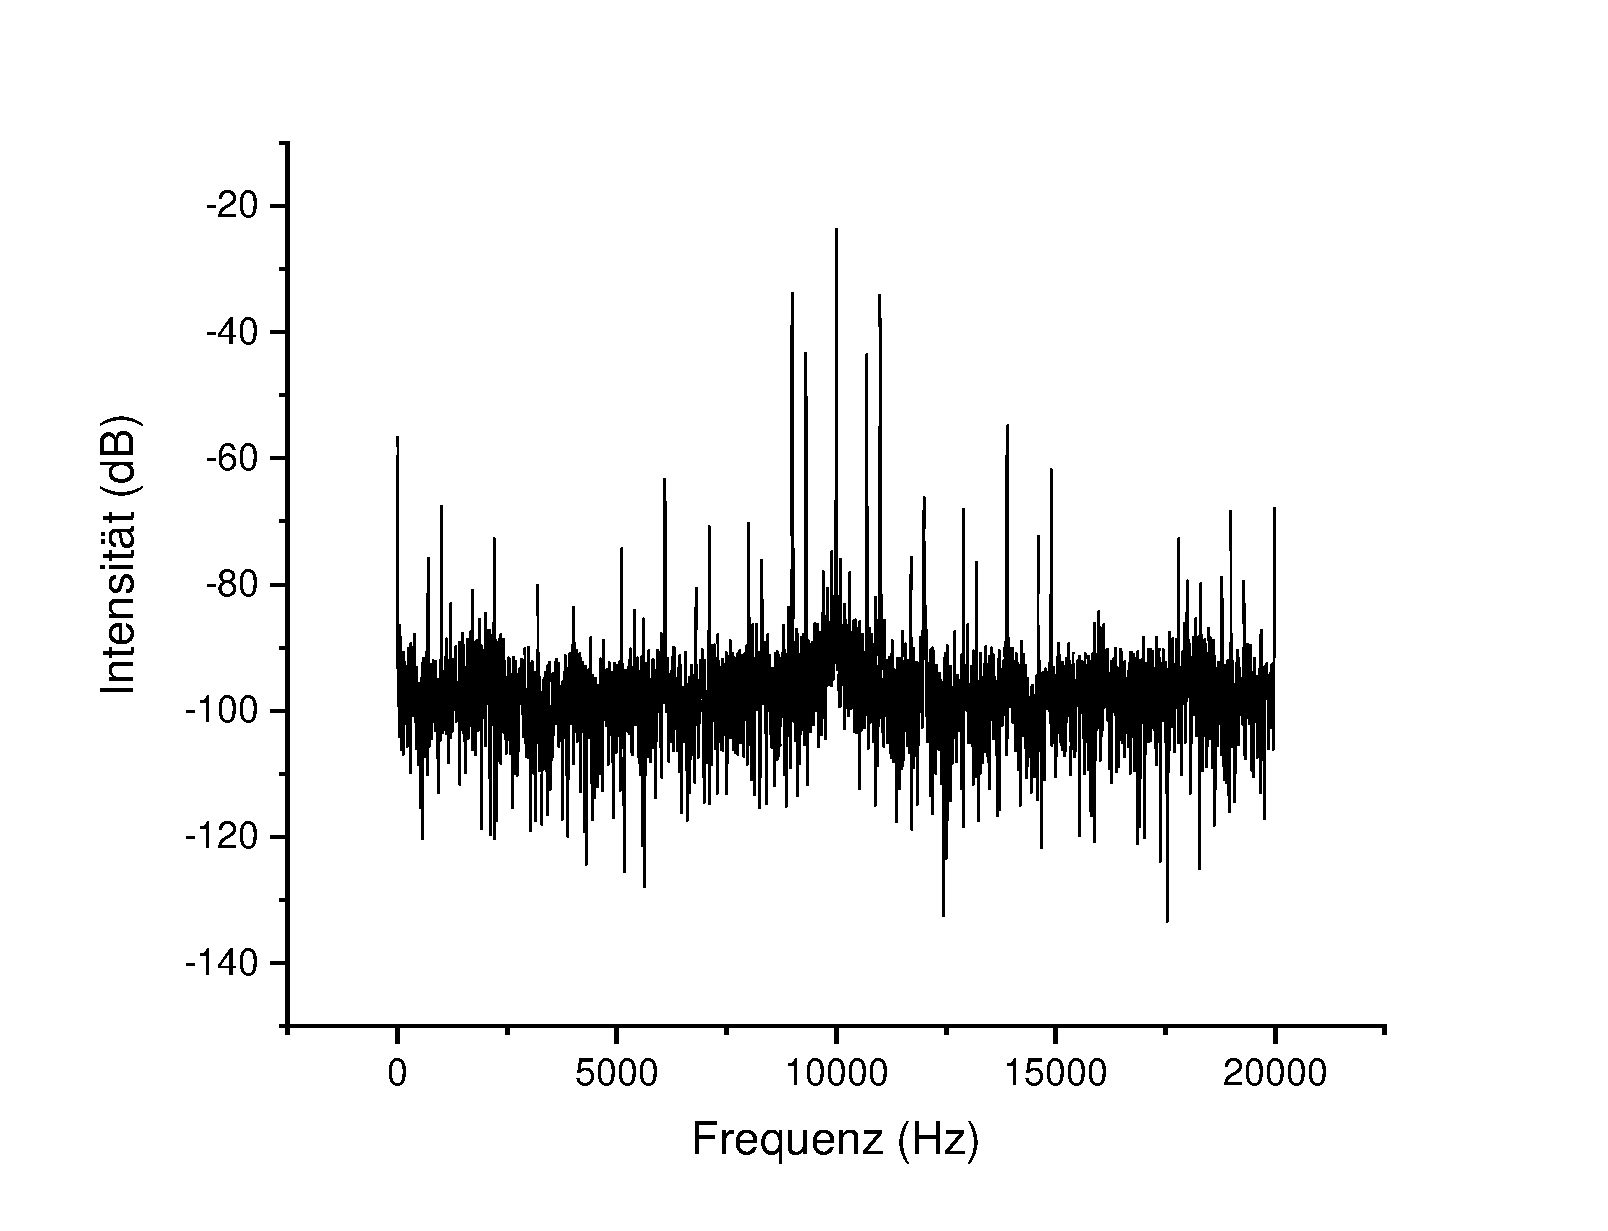
\includegraphics[width=0.7\textwidth]{Origin-Files/AM-Demod-Betrag-Eingang}
		\centering
		\caption{Ausgabe des Oszilloskopprogramms für das Eingangssignal in der Frequenzdomäne bei Eingabe eines amplitudenmodulierten Signals.
		Hierbei fällt auf, dass die Leistung des Trägersignals bei \SI{10000}{\hertz} am stärksten ist. Außerdem sind unmittelbar daneben Summen- und Differenzenfrequenzen des Trägersignals mit den beiden Signalfrequenzen bei \SI{9000}{\hertz}, \SI{9300}{\hertz}, \SI{10700}{\hertz} und \SI{11000}{\hertz} zu sehen.
		}
		\label{fig_tag3_am_demod_eingang}
		\centering
	\end{figure}

	\begin{figure}[H]  
		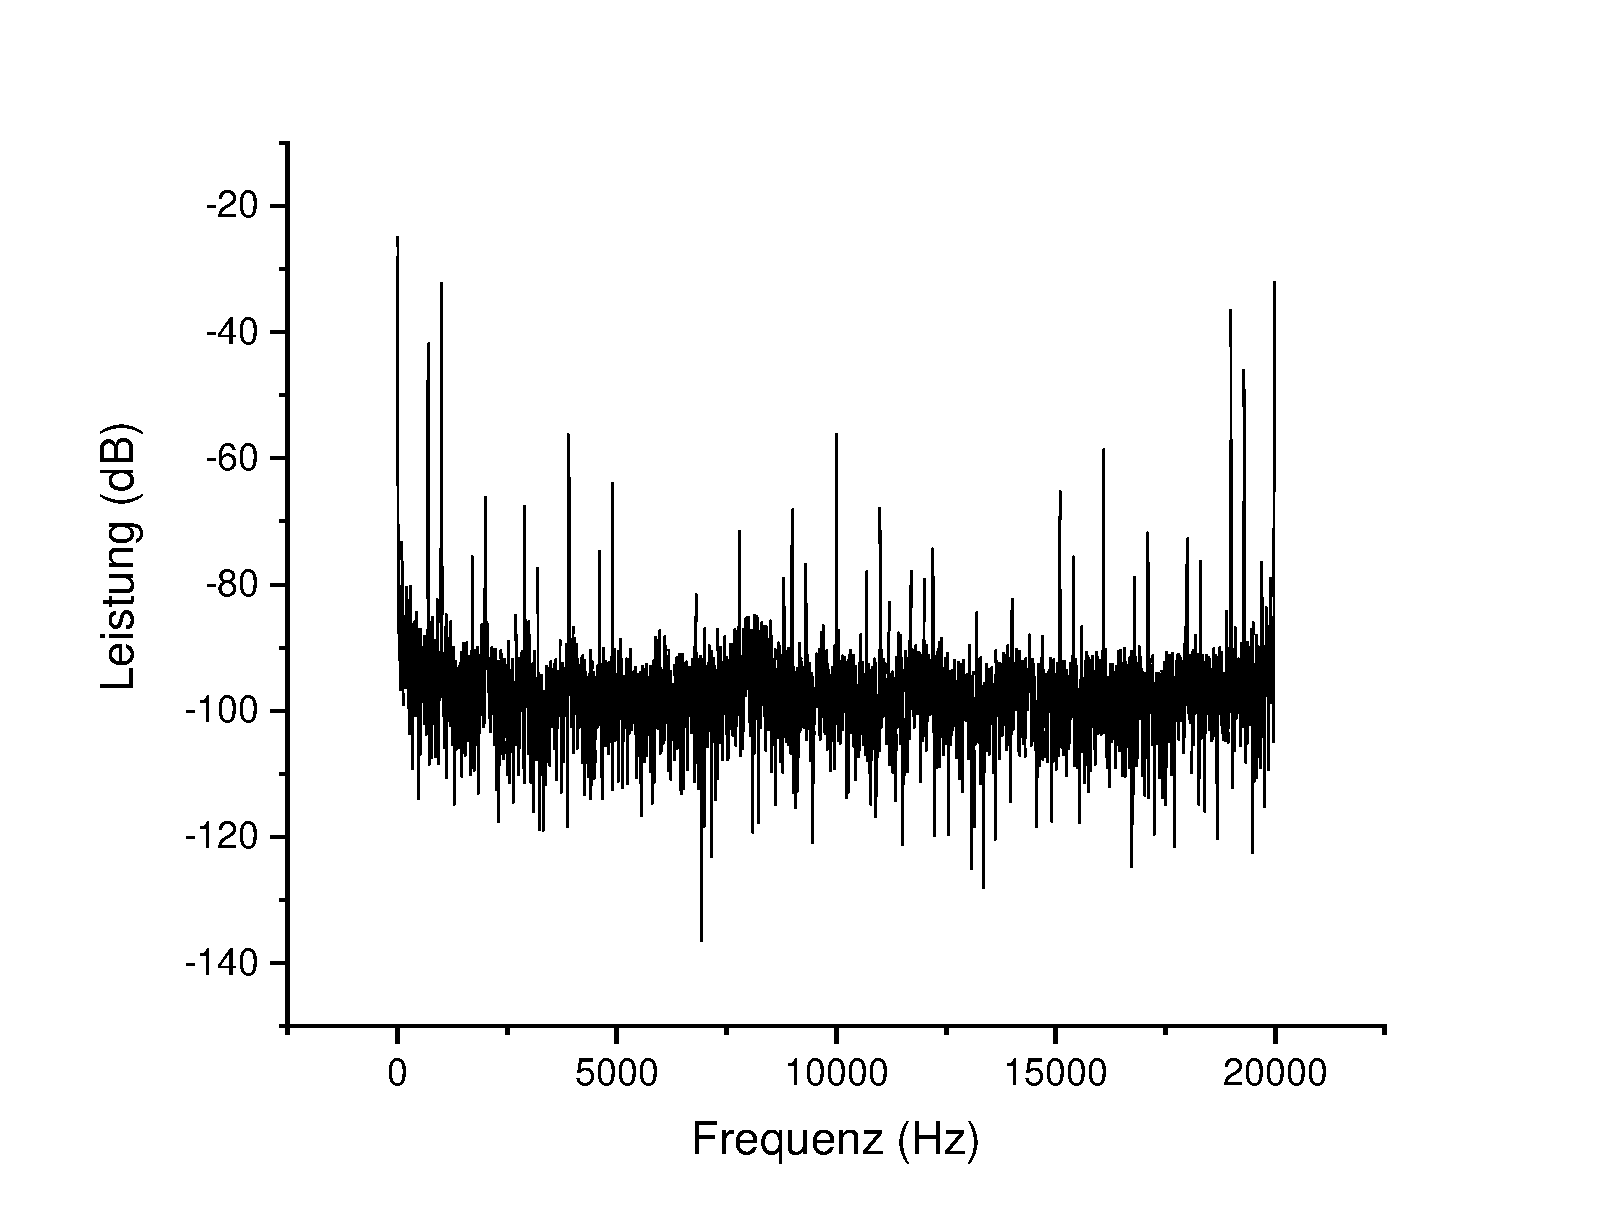
\includegraphics[width=0.7\textwidth]{Origin-Files/AM-Demod-Betrag-preTP}
		\centering
		\caption{Ausgabe des Oszilloskopprogramms in der Frequenzdomäne nach Bilden des Betrags eines amplitudenmodulierten Signals. Die Tiefpassfilterung wurde noch nicht durchgeführt.
		Dass hierin bei \SI{700}{\hertz} und \SI{1000}{\hertz} bereits die Signalfrequenzen vorhanden sind, kann nur festgestellt werden, wenn bereits bekannt ist, wo diese liegen.
		}
		\label{fig_tag3_am_demod_betrag_preTP}
		\centering
	\end{figure}

	\begin{figure}[H]
		\centering
		\begin{subfigure}[t]{0.5\textwidth}
			\centering
			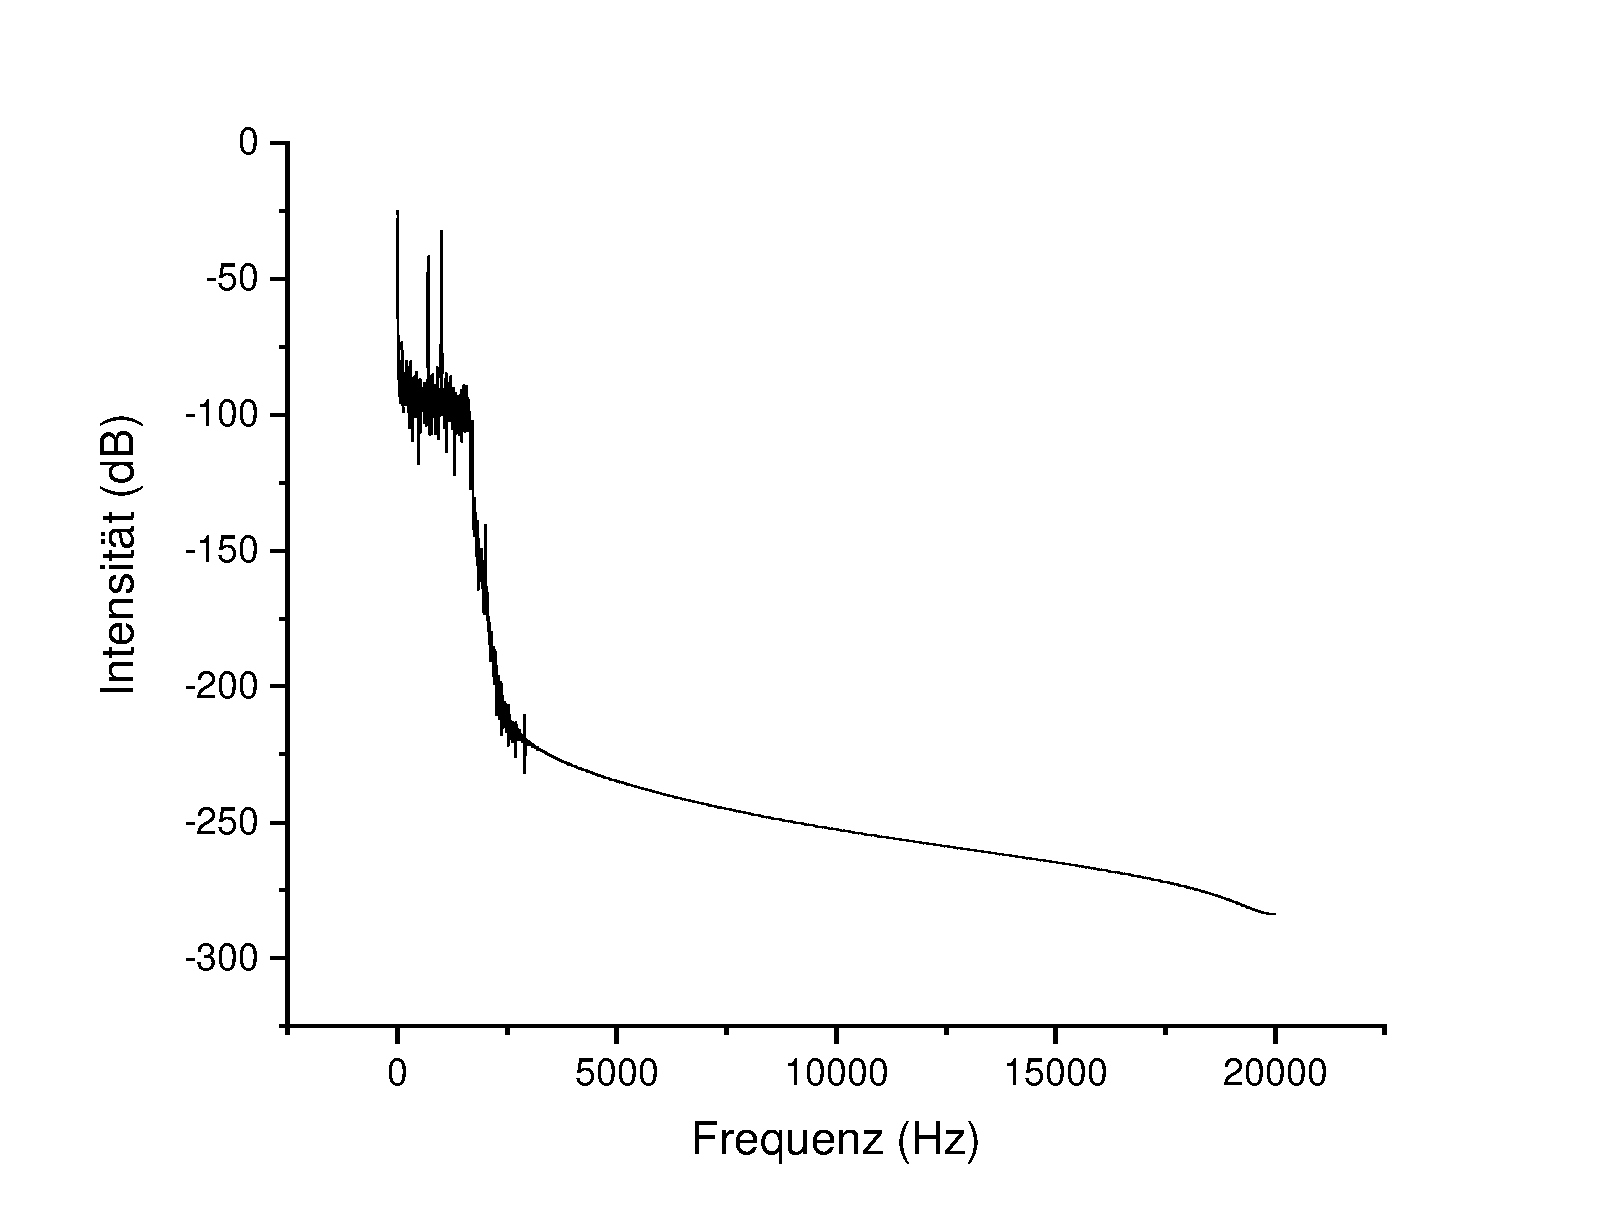
\includegraphics[width=1\textwidth]{Origin-Files/AM-Demod-Betrag-demod}
			\caption{gesamter Frequenzbereich}
		\end{subfigure}%
		\begin{subfigure}[t]{0.5\textwidth}
			\centering
			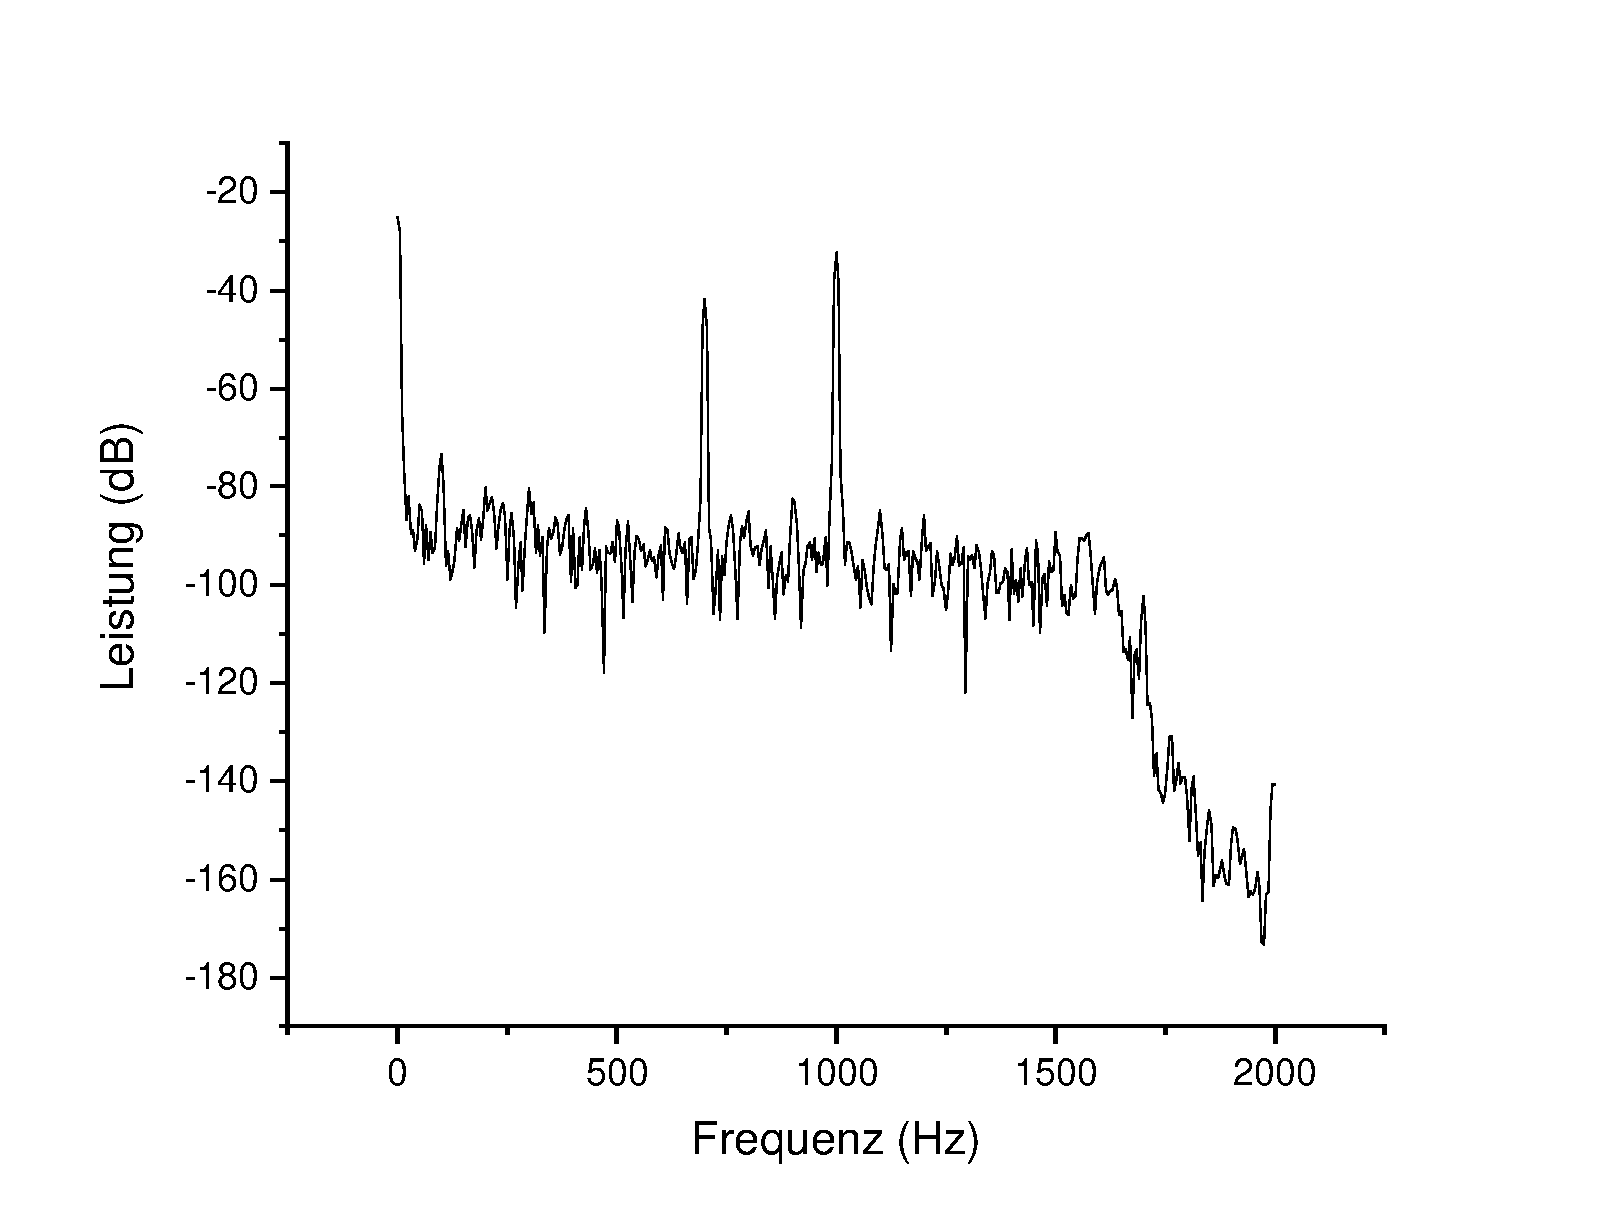
\includegraphics[width=1\textwidth]{Origin-Files/AM-Demod-Betrag-demod-Bereich}
			\caption{geringer Frequenzbereich}
		\end{subfigure}
		\label{fig_tag3_am_demod_betrag_vollst}
		\caption{Ausgabe des Oszilloskopprogramms in der Frequenzdomäne nach vollständiger Demodulation durch Bilden des Betrags und Tiefpassfilterung des amplitudenmodulierten Signals.
		Als Grenzfrequenz für den Tiefpass wurde \SI{1600}{\hertz} gewählt.
		Hierfür muss man voraussetzen, dass bekannt ist, in welchem Frequenzbereich sich die Frequenzen im Signal befinden.
		In der Darstellung des Frequenzbereichs von \SIrange{0}{2000}{\hertz} sind beide Signalfrequenzen sowie ein signifikanter Gleichanteil zu erkennen. % ja den könnte man mit Hochpass wegmachen, muss man das erwähnen? denke nicht - Jannik: muss da nicht hin, ansonsten könnte man sich als Leser fragen, warum man den nicht schon benutzt hat.
		}
		\centering
	\end{figure}



\iffalse %auskommentiert, weil natürlich gleich wie Betrag
	\begin{figure}[H]  
		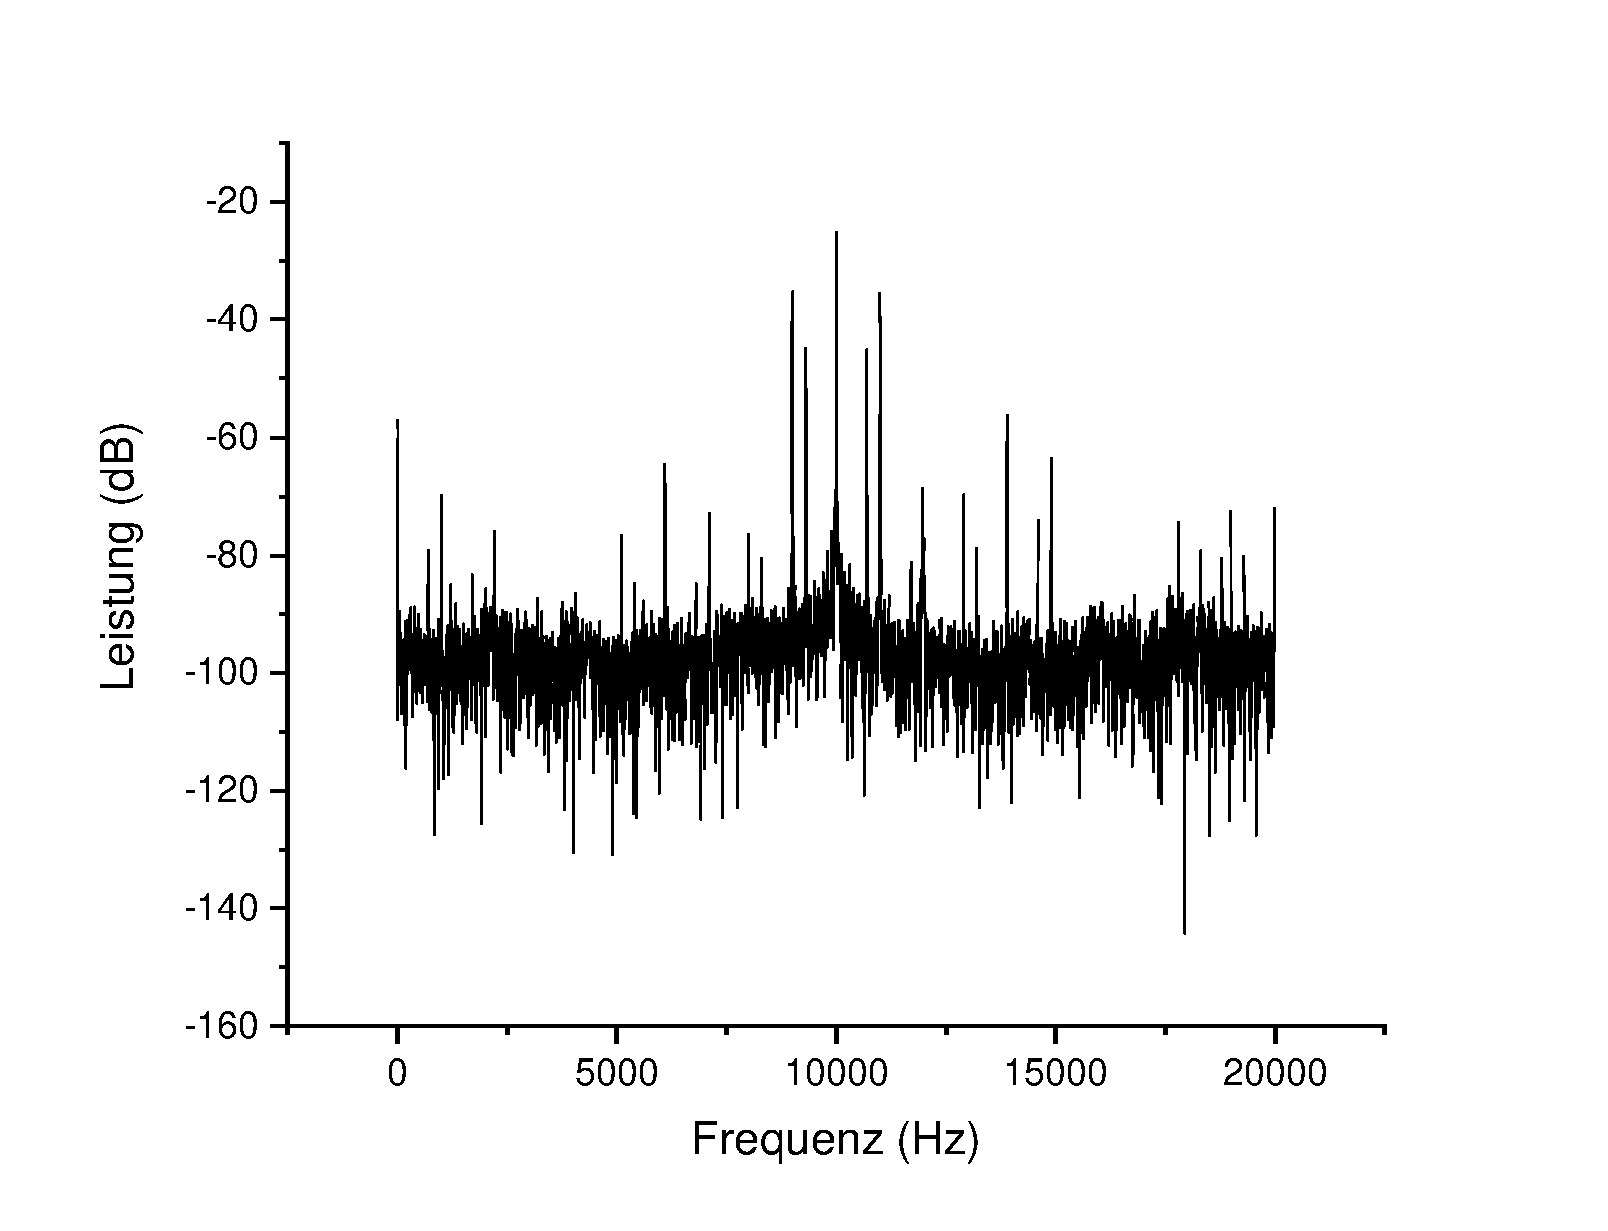
\includegraphics[width=0.7\textwidth]{Origin-Files/AM-Demod-Quadrat-Eingang}
		\centering
		\caption{abc
		}
		\label{}
		\centering
	\end{figure}
\fi

	\begin{figure}[H]  
		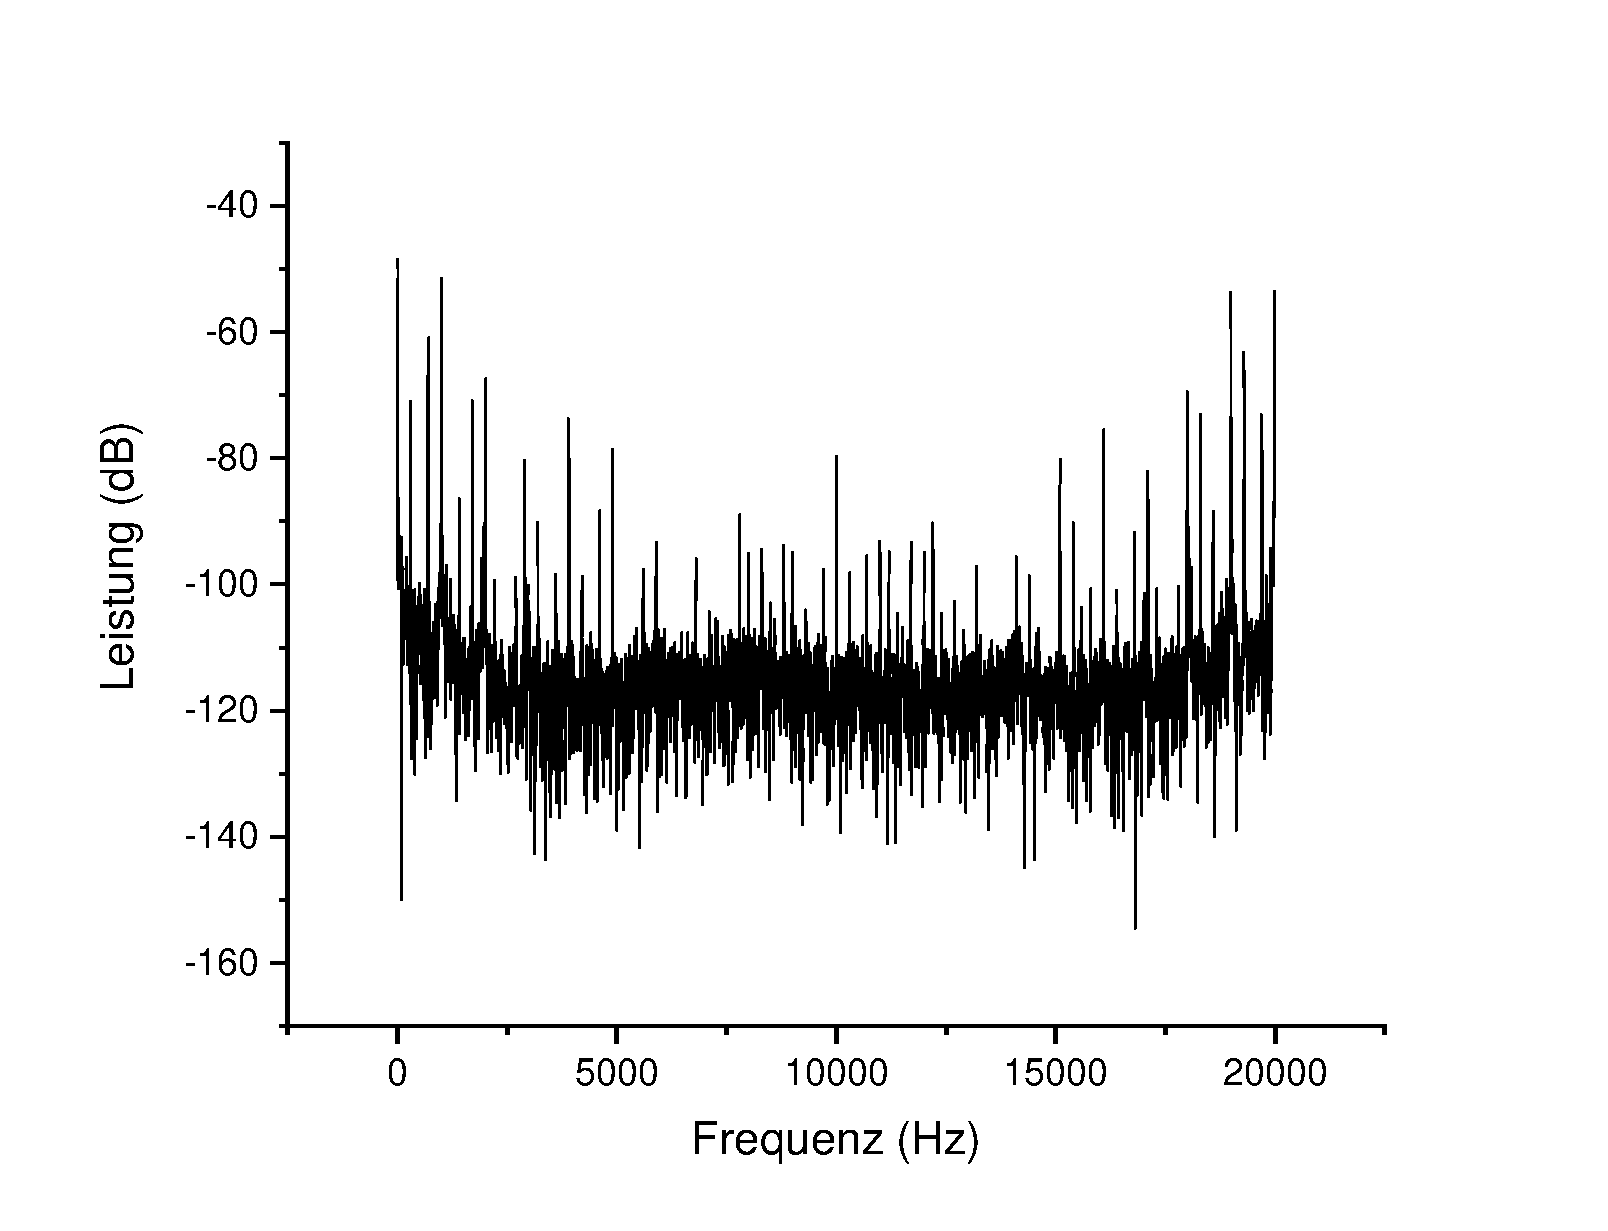
\includegraphics[width=0.7\textwidth]{Origin-Files/AM-Demod-Quadrat-preTP}
		\centering
		\caption{Ausgabe des Oszilloskopprogramms in der Frequenzdomäne nach Quadrieren eines amplitudenmodulierten Signals. Die Tiefpassfilterung wurde noch nicht durchgeführt.
		Dass hierin bei \SI{700}{\hertz} und \SI{1000}{\hertz} bereits die Signalfrequenzen vorhanden sind, kann nur festgestellt werden, wenn bereits bekannt ist, wo diese liegen.
		}
		\label{fig_tag3_am_demod_quadrat_preTP}
		\centering
	\end{figure}

	\begin{figure}[H]
		\centering
		\begin{subfigure}[t]{0.5\textwidth}
			\centering
			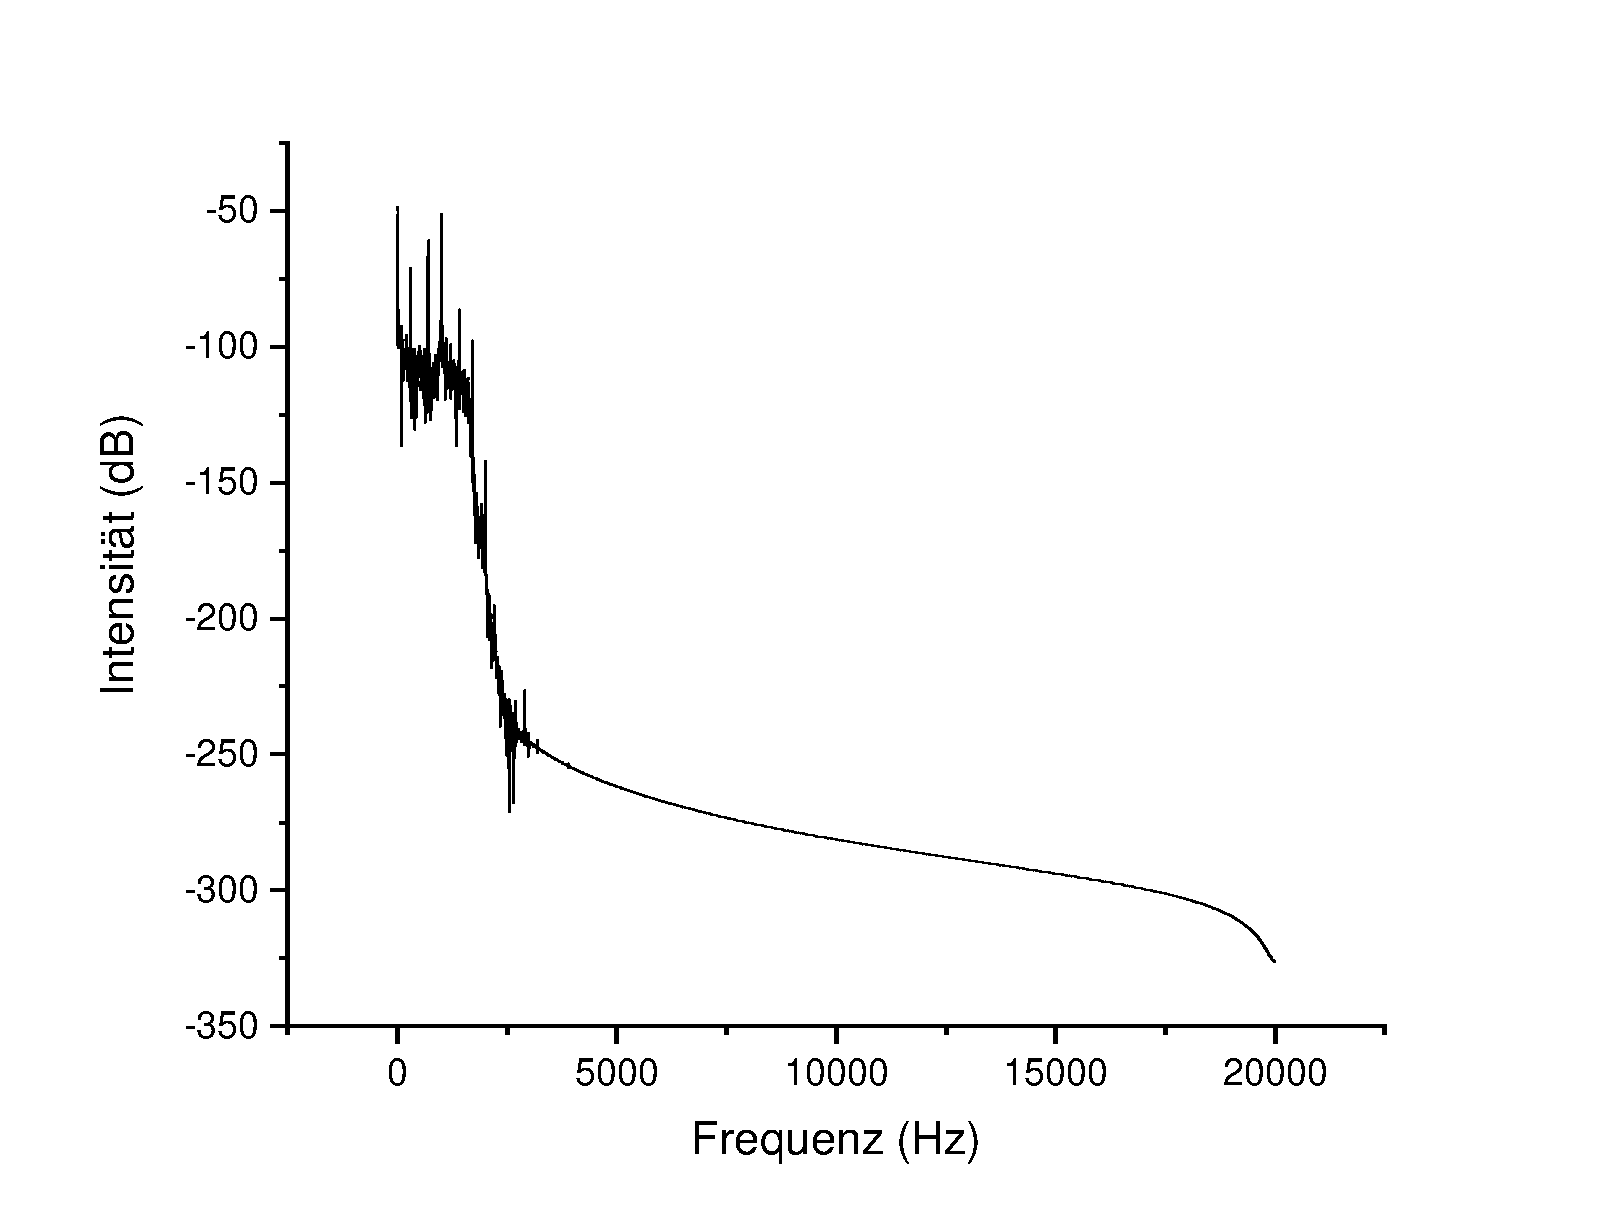
\includegraphics[width=1\textwidth]{Origin-Files/AM-Demod-Quadrat-demod}
			\caption{gesamter Frequenzbereich}
		\end{subfigure}%
		\begin{subfigure}[t]{0.5\textwidth}
			\centering
			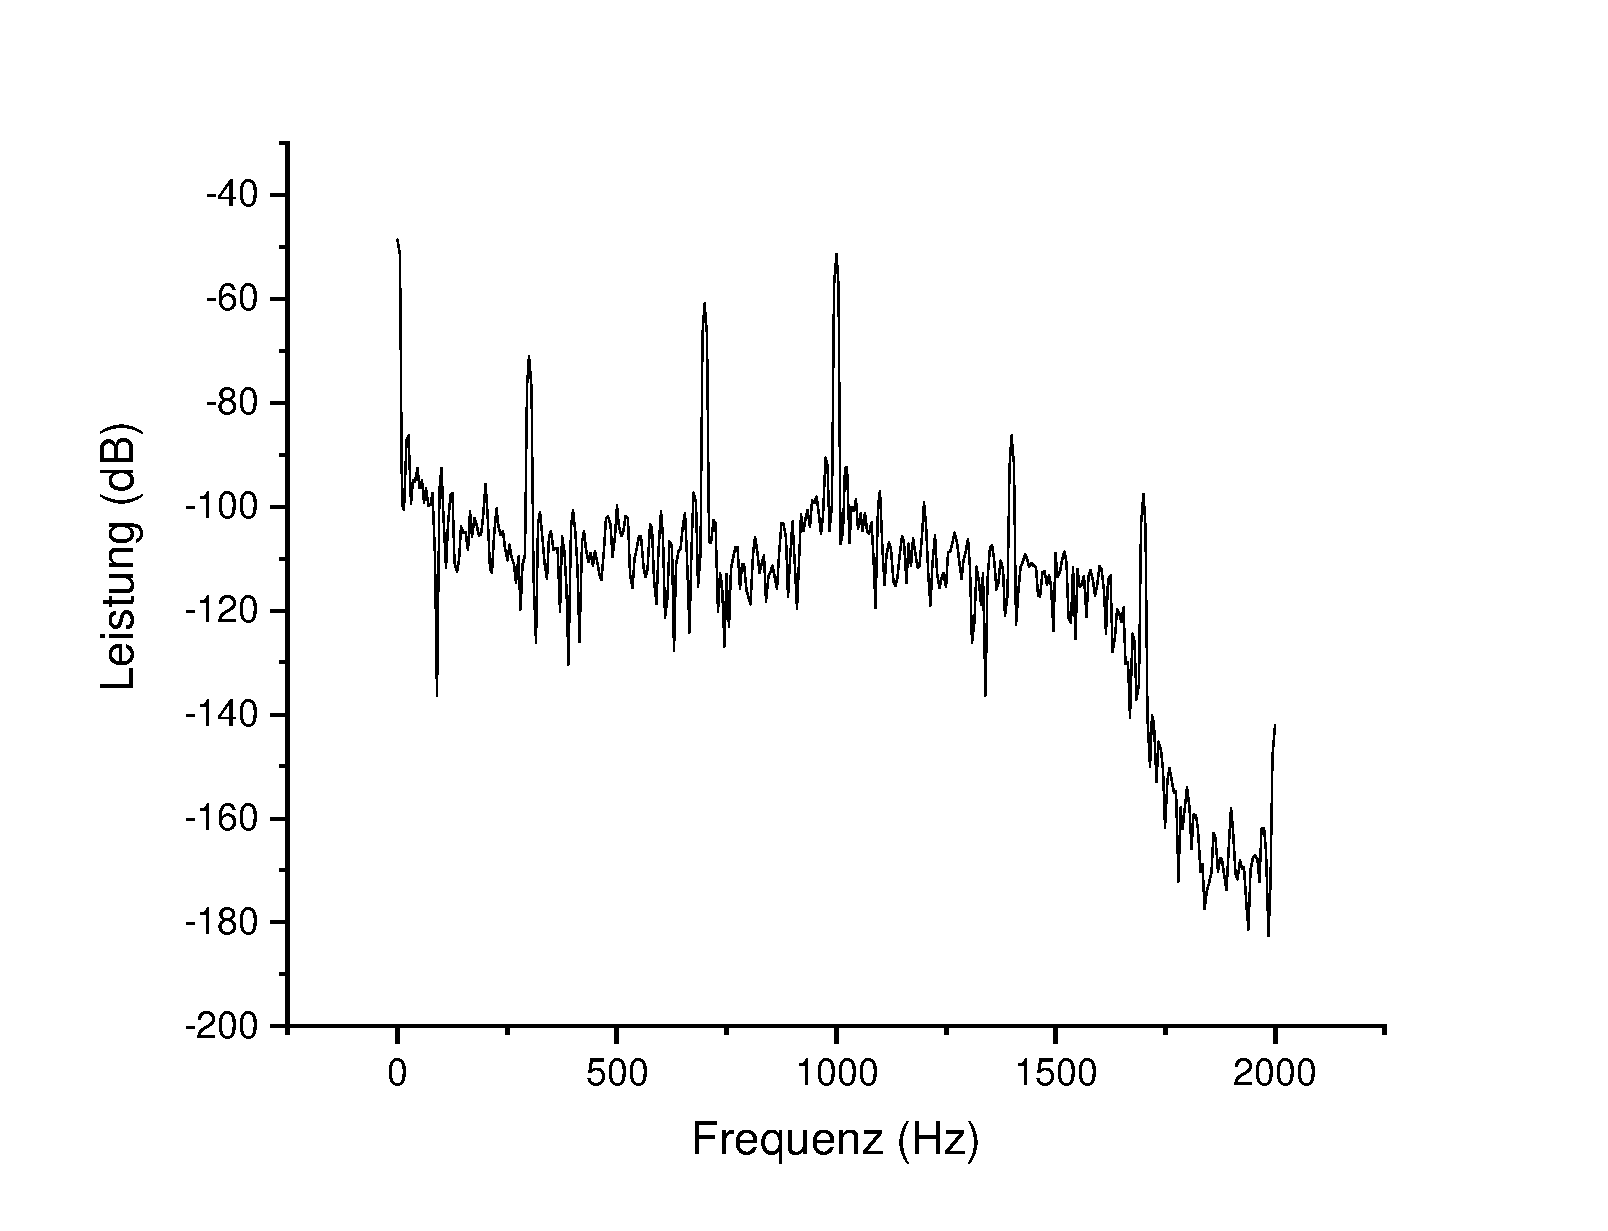
\includegraphics[width=1\textwidth]{Origin-Files/AM-Demod-Quadrat-demod-Bereich}
			\caption{geringer Frequenzbereich}
			\label{fig_tag3_am_demod_quadrat_vollst}
		\end{subfigure}
	
		\caption{Ausgabe des Oszilloskopprogramms in der Frequenzdomäne nach vollständiger Demodulation durch Quadrieren und Tiefpassfilterung des amplitudenmodulierten Signals.
		Als Grenzfrequenz für den Tiefpass wurde \SI{1600}{\hertz} gewählt.
		Hierfür muss man voraussetzen, dass bekannt ist, in welchem Frequenzbereich sich die Frequenzen im Signal befinden.
		In der Darstellung des Frequenzbereichs von \SIrange{0}{2000}{\hertz} sind beide Signalfrequenzen sowie ein signifikanter Gleichanteil zu erkennen.
		Hier treten allerdings noch einige zusätzliche Frequenzen auf, weshalb die Bildung des Betrages gegenüber dem Quadrieren zu bevorzugen ist.
		}
		\centering
	\end{figure}



	\subsection{Demodulation eines AM-Signals mittels Trägerfrequenzmultiplikation} \label{DemodTraeger}
	
	Das allgemeine Ziel dieses Abschnitts ist die Demodulation eines von der Computer-Soundkarte ausgegebenen und anschließend über den Analog-Digital-Wandler gemessenen, amplitudenmodulierten Signals unter Zuhilfenahme der Multiplikation mit der Trägerfrequenz.
	Mathematisch führt das Multiplizieren der amplitudenmodulierten Signal-Funktion mit der Trägerfunktion, welche lediglich der Trägerfrequenz des AM-Signals unterliegt, dazu, dass sich mit dem passenden Additionstheorem als Ergebnis eine Überlagerung bzw. additive Aneinanderreihung von Schwingungstermen unterschiedlichster Frequenzen bildet.
	Letztere lassen sich unter Verwendung einer Fourier-Transformation im Frequenzspektrum dieser Überlagerung betrachten.
	Neben den diversen Peaks an Stellen mit vergleichsweise hohen Frequenzen, ergeben sich darin ebenfalls Peaks bei relativ niedrigen Frequenzwerten. %Link auf Diagramm? - Jannik: Warum hier schon Bezug auf das Diagramm nehmen, wenn ich erst die Theorie dahinter erkläre? >> Na weil du das Diagramm schon beschreibst. Da ist es als Leser schön, schon zu wissen, wovon du redest.
	Demnach handelt es sich um ein breites Frequenzspektrum, in dem man die Frequenz(en) des modulierten, ursprünglichen Signals deutlich erkennen kann.
	Von einem theoretischen Standpunkt aus ist die komplette Demodulation des AM-Signals damit abgeschlossen.
	Zusätzlich lassen sich durch einen Tiefpass mit hinreichend großer Grenzfrequenz die hohen Frequenzanteile aus dem Spektrum herausfiltern, sodass letztendlich nur noch die besagten Frequenzen des Signals übrig bleiben, welches es zu ampliutudenmodulieren galt. 
		
	\begin{figure}[H]
		\centering
		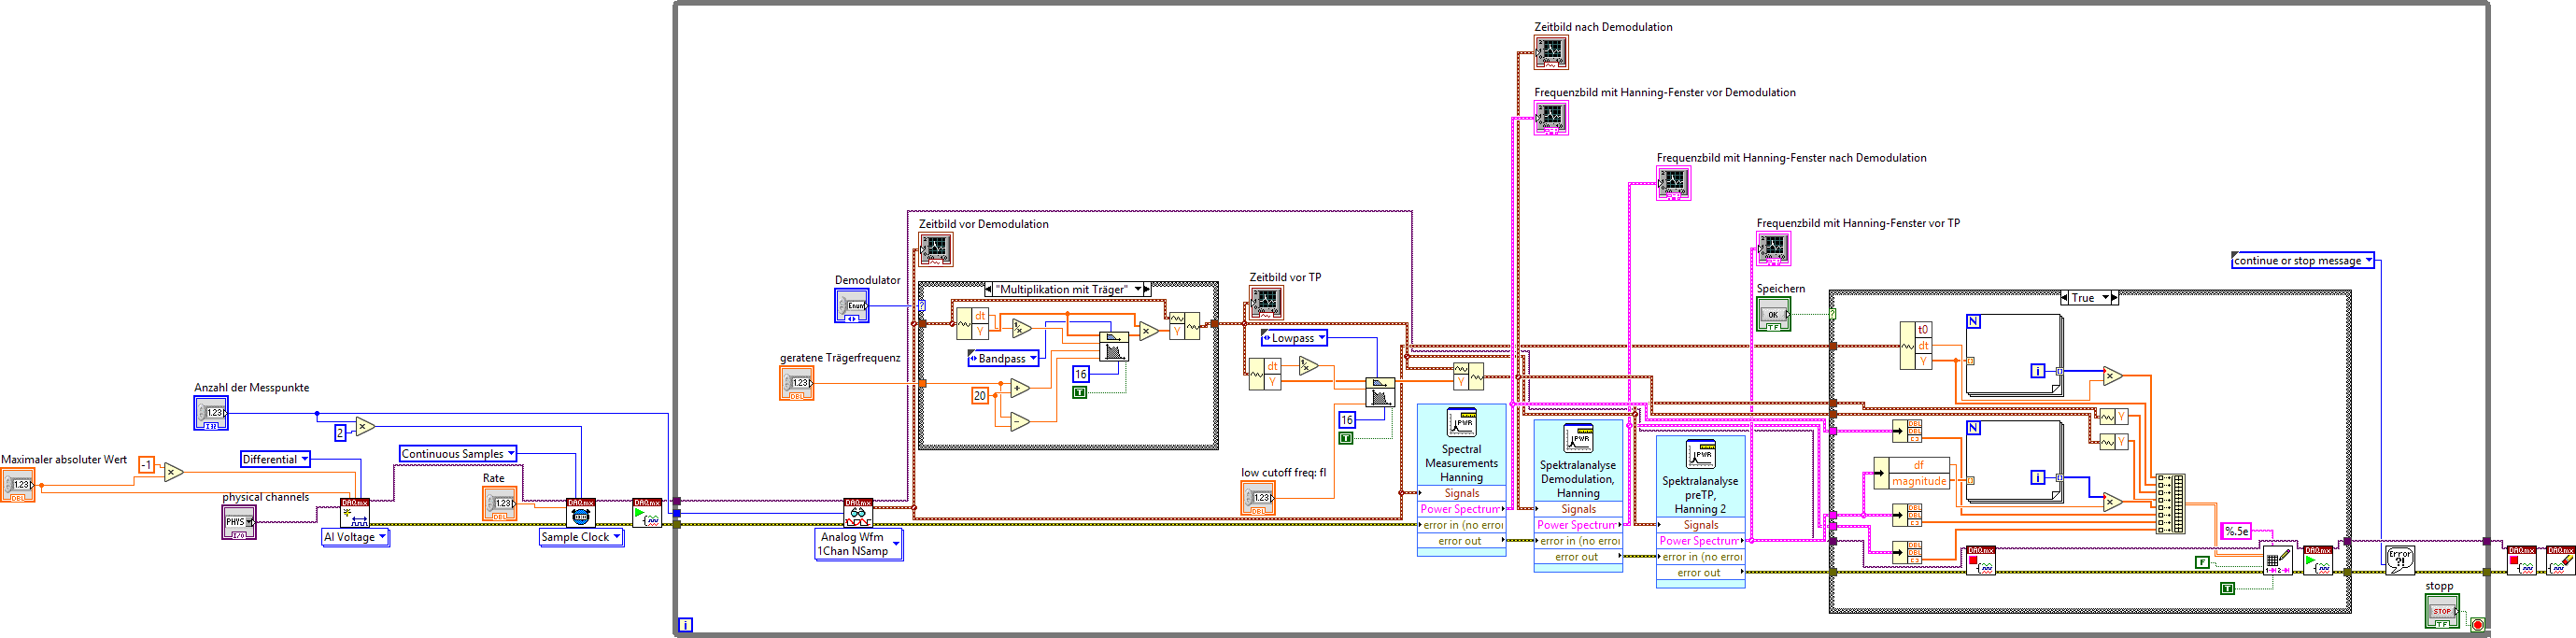
\includegraphics[width=1.0\textwidth]{EIRE2018Dateien/Tag4/traegerMultOszi/Oszilloskop__modifiziertd}
		\caption{Die Abbildung zeigt das LabVIEW-Blockdiagramm bzw. den Programmcode zur Demodulation eines von der Computer-Soundkarte ausgegebenen und anschließend über den Analog-Digital-Wandler gemessenen, amplitudenmodulierten Signals mittels Trägerfrequenzmultiplikation.}
		\label{MultiTraegerProgrammcode}
	\end{figure}
	
	Dieses Verfahren soll nun in ein LabVIEW-Programm übertragen werden, dessen zugehöriger Programmcode in \ref{MultiTraegerProgrammcode} zu sehen ist. 
	Voraussetzung ist dabei das in \cref{DemodulationAM} bereits erstellte Programm.
	Alle zuvor eingefügten Methoden zur Demodulation (\glqq Quadrat\grqq\ und \glqq Betrag\grqq ) sollen frei auswählbar bleiben.
	Dafür wird zunächst die Demodulator-Case-Konstruktion um eine weitere Option mit dem Namen \glqq Multiplikation mit Träger\grqq\ ergänzt und somit ein neues, ausfüllbares Case-Feld erzeugt.
	Darin werden diverse, später näher beschriebene Blockdiagrammobjekte angelegt, welche die Demodulation des von der Computer-Soundkarte ausgegebenen und anschließend über den Analog-Digital-Wandler gemessenen, amplitudenmodulierten Signals umsetzten.
	Zuerst muss hierbei vom Nutzer die Trägerfrequenz des amplitudenmodulierten Signals geraten werden.
	Dies entspricht dem Vorgang, bei dem am herkömmlichen UKW-Radio ein Sender eingestellt wird.
	Dazu wird sowohl ein weiteres Bedienelement auf dem Frontpanel hinzugefügt, als auch ein entsprechendes Blockdiagrammobjekt im Programmcode erstellt.
	Mit einem Bandpass sechzehnter Ordnung soll die geratene Trägerfrequenz aus dem Frequenzspektrum des AM-Signals herausgefiltert werden. 
	Die obere bzw. untere Grenzfrequenz des Bandpassfilters bildet der geratene Trägerfrequenzwert zuzüglich bzw. abzüglich eines Werts von \SI{20}{\hertz}. 
	Dieser \SI{20}{\hertz}-Wert ist hinreichend groß gewählt, um einerseits Überlappungen mit anderen Frequenz-Peaks zu vermeiden und andererseits die Gesamtheit des Trägerfrequenz-Peaks zu erfassen. 
	Es wird also ein Bereich von $\pm 20\,$Hz um die Trägerfrequenz \enquote{herausgeschnitten}. 
	Die dazugehörige Schwingungsfunktion wird nun mit dem unveränderten, gemessenen amplitudenmodulierten Signal multipliziert. 
	
	\begin{figure}[H]
		\centering
		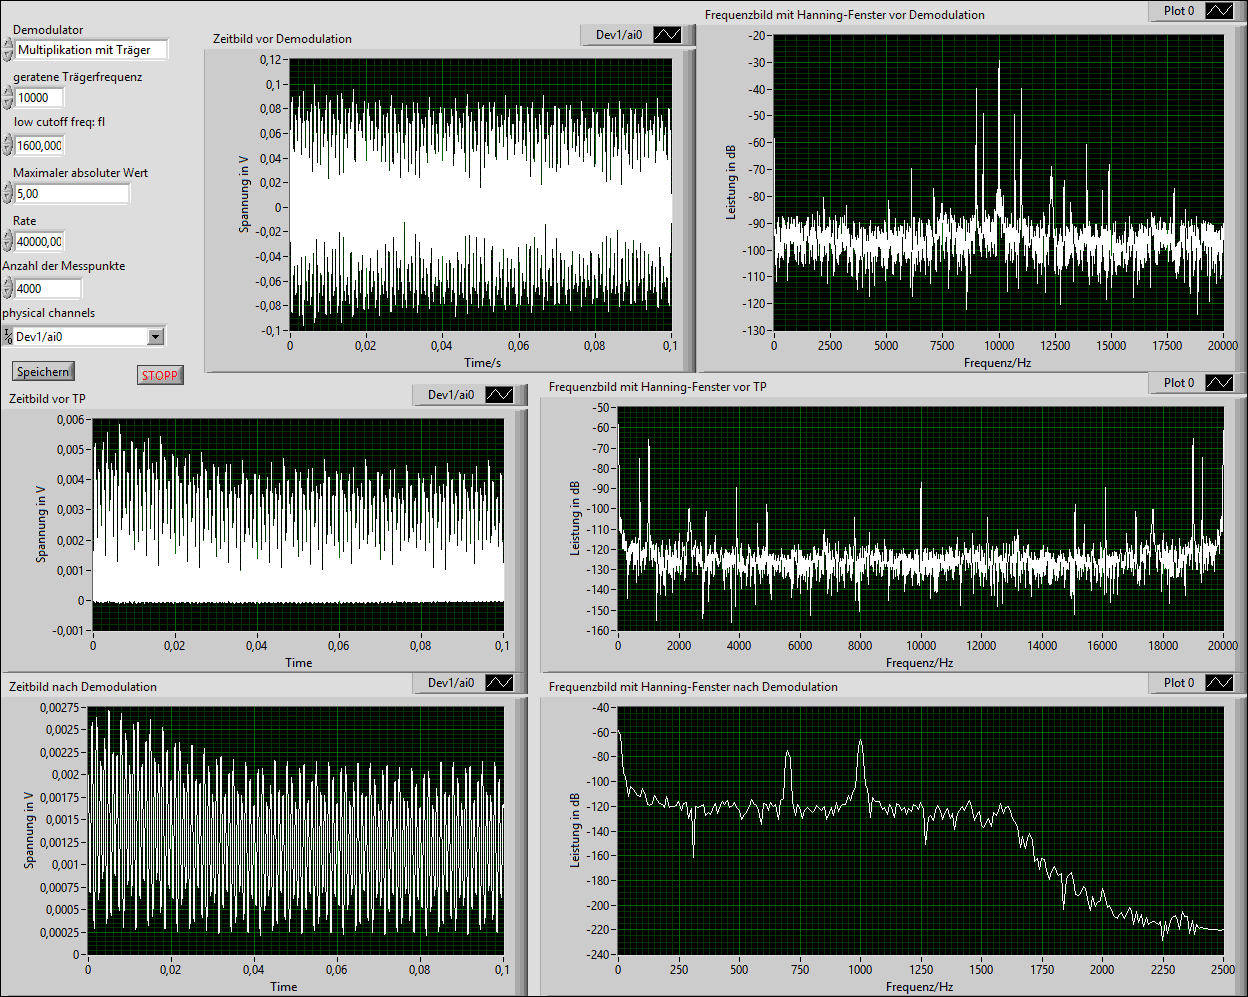
\includegraphics[width=1.0\textwidth]{EIRE2018Dateien/Tag4/traegerMultOszi/Oszilloskop__modifiziertp}
		\caption{Die Abbildung veranschaulicht die LabVIEW-Benutzeroberfläche bzw. das LabVIEW-Frontpanel des Programms zur Demodulation eines von der Computer-Soundkarte ausgegebenen und anschließend über den Analog-Digital-Wandler gemessenen AM-Signals mittels Trägerfrequenzmultiplikation. Alle sechs Anzeige- bzw. Ausgabeelemente zeigen in zweidimensionalen, kartesischen Diagrammen das an bestimmten Stellen des Bearbeitungsprozesses abgegriffene AM-Signal, jeweils im Zeitbild und im Frequenzbild mit Hanning-Fenster. Die beiden oberen Diagramme stellen das von der Computer-Soundkarte ausgegebene und anschließend über den Analog-Digital-Wandler gemessene AM-Signal vor der Demodulation dar. In den beiden mittleren Diagrammen sieht man das Ergebnis der Demodulation des amplitudenmodulierten Signals ohne Tiefpassfilterung. Die unteren beiden Diagramme veranschaulichen das demodulierte AM-Signal nach der Tiefpassfilterung.}
		\label{MultiTraegerFrontpanel}
	\end{figure}
	
	\noindent Das Ergebnis dieser Operation ist, wie zuvor im Theorie-Teil erwähnt, ein breites Frequenzspektrum mit zahlreichen Peaks an unterschiedlich hohen und niedrigen Frequenzwerten, was im rechten, mittleren Diagramm in \cref{MultiTraegerFrontpanel} erkennbar ist. 
	Überdies sind in \cref{MultiTraegerFrontpanel} noch fünf weitere Anzeigeelemente in Diagramm-Form dargestellt: Die beiden Oberen zeigen das von der Computer-Soundkarte ausgegebene und anschließend über den Analog-Digital-Wandler gemessene, amplitudenmodulierte Signal ohne Demodulation, zum einen im Zeitbild und zum andern im Frequenzbild.
	Im linken, mittleren Anzeigeelement ist ein Diagramm zu sehen, in dem der zeitliche Signalverlauf nach der Durchführung der Trägerfrequenzmultiplikation und somit auch nach der kompletten Demodulation veranschaulicht ist. 
	Die beiden unteren Anzeigeelemente stellen, sowohl im Zeit- als auch im Frequenzbild, das demodulierte AM-Signal nach der bereits im Theorie-Teil angesprochenen Tiefpassfilterung dar. 
	Genauso wie in \cref{DemodulationAM} findet die Tiefpassfilterung außerhalb der Demodulator-Case-Konstruktion statt. 
	Dabei bedarf es eines zusätzlichen Bedienelements auf dem Frontpanel sowie eines dazugehörigen Blockdiagrammobjekts im Programmcode, um die entsprechende Grenzfrequenz für den Tiefpass festzulegen. 
	Diese liegt in \cref{MultiTraegerFrontpanel} bei $1.600\,$Hz. 
	Zudem befinden sich auf der Benutzeroberfläche in \cref{MultiTraegerFrontpanel} sämtliche Bedien- bzw. Eingabeelemente oben links.
	
	Das für den in \cref{MultiTraegerFrontpanel} gezeigten Programmdurchlauf verwendete Signal, welches in \cref{AMSignalErzeugung} amplitudenmoduliert wurde und dieselbe Gestalt wie in \cref{Ursprungssignal} besitzt, wird unter anderem durch die Frequenzen $f_1 = 700\,$Hz und $f_2 = 1.000\,$Hz bestimmt. 
	Dies lässt sich insbesondere anhand der Bedienelemente-Einstellung des Frontpanels in \cref{fig_tag3_am_soundkarte_front} nachvollziehen. 
				
	\begin{figure}[H]
		\centering
		\includegraphics[width=1.0\textwidth]{EIRE2018Dateien/Tag4/traegerMultOszi/exaktTraegerRate10000m0,2}
		\caption{In dieser Abbildung ist das Ergebnis einer erfolgreichen Demodulation des von der Computer-Soundkarte ausgegebenen und anschließend über den Analog-Digital-Wandler gemessenen AM-Signals zu sehen. Bei diesem Frequenzbild mit Hanning-Fenster handelt sich um das aus \cref{MultiTraegerFrontpanel} bekannte, rechts unten auffindbare Frontpanel-Diagramm. Der Trägerfrequenz-Wert von $10.000\,$Hz wurde exakt geraten. Der Modulationsgrad des AM-Signals beträgt $0,2$. Die Daten für das hier dargestellte Frequenzspektrum entstammen der durch die Speicherfunktion des LabVIEW-Programms erhaltenen Textdatei und wurden mit dem Datenanalyse-Programm \glqq SciDAVis\grqq\ bearbeitet.}
		\label{AMDemodsuccm02}
	\end{figure}

	\noindent Die Demodulation des von der Computer-Soundkarte ausgegebenen und anschließend über den Analog-Digital-Wandler gemessenen, amplitudenmodulierten Signals mittels Trägerfrequenzmultiplikation sowie die anschließende Tiefpassfilterung führten schlussendlich zu dem Frequenzbild, was unten rechts auf der Benutzeroberfläche in \cref{MultiTraegerFrontpanel} dargestellt ist.
	Dieses Frequenzspektrum weist zwei deutliche Peaks bei $700\,$Hz und $1.000\,$Hz auf, welche genau den $f_1$- und $f_2$-Werten des zu amplitudenmodulierenden Signals entsprechen. 
	Daher kann man als Fazit sagen, dass es sich wohl um eine erfolgreich funktionierende Amplitudenmodulation sowie Demodulation handelt. 
	
	Anzumerken ist noch, dass bei einem größer gewählten Modulationsgrad $m$ in \cref{AMFormel} die Peaks im Frequenzspektrum bei den eingestellten $f_1$- und $f_2$-Werten höher ausfallen und damit leichter zu erkennen sind. 
	
	\begin{figure}[H]
		\centering
		\includegraphics[width=1.0\textwidth]{EIRE2018Dateien/Tag4/traegerMultOszi/exaktTraegerRate10000m1,2}
		\caption{Die Abbildung veranschaulicht das Ergebnis einer erfolgreichen Demodulation des von der Computer-Soundkarte ausgegebenen und anschließend über den Analog-Digital-Wandler gemessenen AM-Signals bei einem Modulationsgrad von $m = 1,2$. Bei diesem Frequenzbild mit Hanning-Fenster handelt sich um das aus \cref{MultiTraegerFrontpanel} bekannte, rechts unten auffindbare Frontpanel-Diagramm. Der Trägerfrequenz-Wert von $10.000\,$Hz wurde exakt geraten. Die Daten für das hier dargestellte Frequenzspektrum entstammen der durch die Speicherfunktion des LabVIEW-Programms erhaltenen txt-Datei und wurden mit dem Datenanalyse-Programm \glqq SciDAVis\grqq\ bearbeitet.}
		\label{AMDemodsuccm12}
	\end{figure}

	\noindent Dieser Effekt wird vor allem beim Vergleich von \cref{AMDemodsuccm02} mit \cref{AMDemodsuccm12} deutlich. 
	Hierbei liegt eine Versechsfachung des Modulationsgrads $m$ vor.
	
	Anhand der \cref{AMDemodfailm02} lässt sich erkennen, welche Folgen sich beim Versuch der Demodulation ergeben, sobald man die (geratene) Trägerfrequenz zu weit außerhalb des $\pm 20\,$Hz-Bereichs wählt.
	Hierbei wurde der Trägerfrequenz-Wert nämlich auf $10.050\,$Hz geraten, gleichwohl die tatsächliche Trägerfrequenz des AM-Signals bei $10.000\,$Hz liegt.
	Bei dem in \cref{AMDemodfailm02} gezeigten Frequenzbild mit Hanning-Fenster, welches äquivalent zum aus \cref{MultiTraegerFrontpanel} bekannten, sich rechts unten befindenden Frontpanel-Diagramm ist, kann man daher nicht die beiden vom ursprünglichen Signal stammenden Frequenzen $f_1 = 700\,$Hz und $f_2 = 1.000\,$Hz ablesen.
	Denn bei diesen Frequenz-Werten sind keine Peaks zu sehen.
	
	\begin{figure}[H]
		\centering
		\includegraphics[width=1.0\textwidth]{EIRE2018Dateien/Tag4/traegerMultOszi/nichtexaktTraegerRate10050m0,2}
		\caption{Die Abbildung zeigt das Ergebnis einer misslungenen Demodulation des von der Computer-Soundkarte ausgegebenen und anschließend über den Analog-Digital-Wandler gemessenen AM-Signals. Der geratenen Trägerfrequenz-Wert liegt bei $10.050\,$Hz, die tatsächliche Trägerfrequenz des AM-Signals beträgt jedoch $10.000\,$Hz. Der Wert des Modulationsgrads lautet $0,2$. Die Daten für das hier dargestellte Frequenzspektrum entstammen der durch die Speicherfunktion des LabVIEW-Programms erhaltenen txt-Datei und wurden mit dem Datenanalyse-Programm \glqq SciDAVis\grqq\ bearbeitet.}
		\label{AMDemodfailm02}
	\end{figure}

	\noindent Stattdessen lassen sich in dem Teil des Frequenzspektrums, der nach der Tiefpassfilterung übrig geblieben ist, einige verstreute Peaks unterschiedlicher Höhe und Breite an verschiedenen Frequenz-Werten lokalisieren.
	Folglich ist die Demodulation mittels Trägerfrequenzmultiplikation in diesem Fall nicht gelungen.
	
	\newpage
	
	
	\section{Phasen- und frequenzmodulierte Signale}

	\subsection{Erzeugung eines phasen- bzw. frequenzmodulierten Signals} \label{FMPMErzeugung} %Bilderanordnung schön, bitte so lassen.
	
	%Allgemeiner Absatz:
	In diesem Abschnitt soll ein LabVIEW-Programm entstehen, welches ein Signal der in \cref{Ursprungssignal} präsentierten Form zunächst wahlweise phasen- oder frequenzmoduliert und anschließend über die Soundkarte des verwendeten Computers ausgibt. 
	Der daraus hervorgehende Programmcode ist in \cref{FMProgrammcode} und \cref{PMProgrammcode} aufgeführt.
	
	\begin{figure}[H]
		\centering
		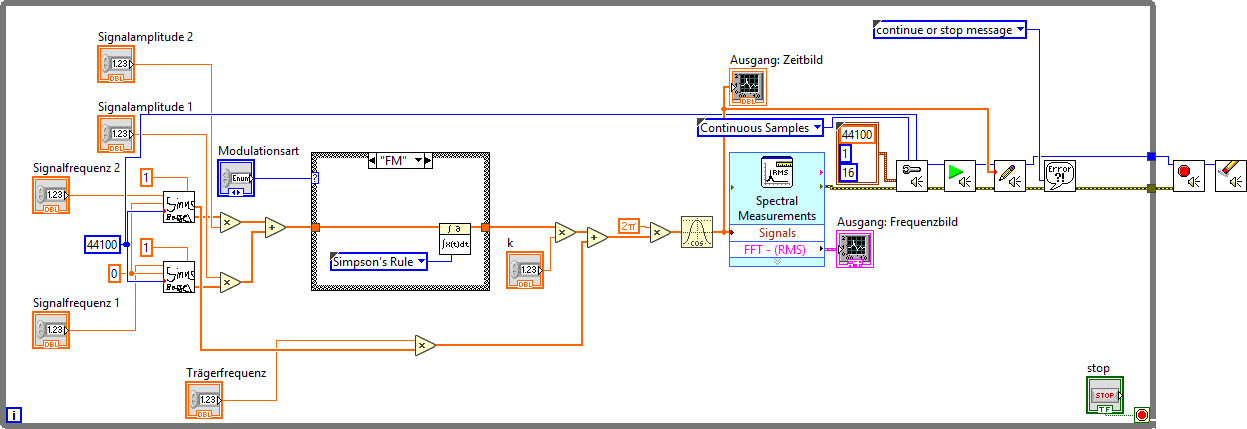
\includegraphics[width=1.0\textwidth]{EIRE2018Dateien/Tag4/FMPM-Erzeugung/FMPM-Erzeugungd}
		\caption{In dieser Abbildung ist das LabVIEW-Blockdiagramm bzw. der Programmcode zu sehen, mit dem ein Signal zuerst wahlweise phasen- oder frequenzmoduliert und anschließend über die Computer-Soundkarte ausgeben wird.}
		\label{FMProgrammcode}
	\end{figure}
	
	\noindent Bei der dazugehörigen Benutzeroberfläche, welche in \cref{FMAusgabekleinesk}, \cref{FMAusgabegrossesk} sowie \cref{PMAusgabe} dargestellt ist, befinden sich alle Bedien- bzw. Eingabeelemente auf der linken und alle Anzeige- bzw. Ausgabeelemente auf der rechten Seite.
	
	\begin{figure}[H]
		\centering
		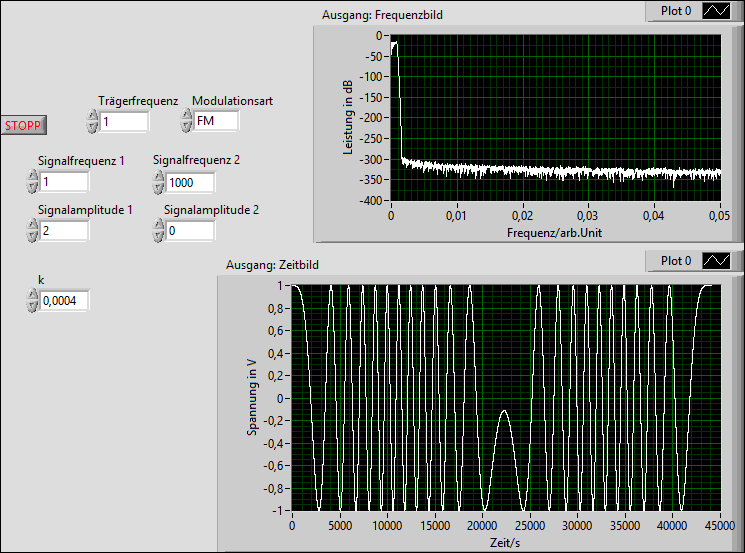
\includegraphics[width=1.0\textwidth]{EIRE2018Dateien/Tag4/FMPM-Erzeugung/FM-FMPM-Erzeugungp}
		\caption{Die Abbildung zeigt das Frontpanel bzw. die Benutzeroberfläche des LabVIEW-Programms zur Umsetzung der Frequenzmodulation. Der hierbei verwendete $k$-Wert ist sehr klein. Allgemein besteht mit dem entsprechenden, sich oben auf dem Frontpanel befindenden Bedienelement die Möglichkeit die Art der Modulation auszuwählen: Entweder Frequenzmodulation (Abkürzung: FM) oder Phasenmodulation (Abkürzung: PM).}
		\label{FMAusgabekleinesk}
	\end{figure}
	
	\noindent In diesem Fall handelt es sich bei den Anzeigeelementen um zwei Diagramme, die das phasen- oder frequenzmodulierte Signal, je nachdem welche Modulationsart ausgewählt ist, im Zeit- und Frequenzbild anzeigen. 
	Die Blockdiagrammobjekte, welche die Ausgabe über die Computer-Soundkarte realisieren, liegen rechtsseitig im Programmcode und teilweise außerhalb der While-Schleife. 
	Deren Anordnung und Funktionsweise ist die gleiche wie beim LabVIEW-Programm in \cref{AMSignalErzeugung}. 
	Genauso wie in \cref{fig_tag3_am_soundkarte_block} aus \cref{AMSignalErzeugung} sieht man auf der linken Seite des Programmcodes zunächst die Erzeugung des Signals $s(t)$ gemäß \cref{Ursprungssignal} mit den Frequenzen $f_1$ und $f_2$. 
	Weiterhin ist dabei die zusätzliche, aufgrund des in \cref{sinusfkt} aufgetretenen Programmierfehlers notwendige nachträgliche Multiplikation mit der Amplitude zu beachten. 
	Außerdem soll $N = 44.100$ gelten. 
	Da der Vorgang der $s(t)$-Konstruktion komplett identisch zu der in \cref{AMSignalErzeugung} bereits ausführlich beschriebenen Vorgehensweise ist, wird an dieser Stelle nicht weiter auf die Signalentstehung eingegangen. 
	Die gesamte Berechnung (FM- und PM-Modulation sowie Signalerzeugung) und der Großteil der Signalausgabe finden in einer While-Schleife statt, was auch aus \cref{FMProgrammcode} hervorgeht.
	Ebenso wie bei den zuvor behandelten Abschnitten ist der While-Schleife ein \glqq Stopp\grqq -Knopf beigefügt, um das Programm bei Bedarf anhalten zu können.
	Zwischen den Blockdiagrammobjekten zur Benutzeroberflächenkonfiguration und der Signalentstehung findet im Programmcode die Modulation des Signals statt.
	Durch das Hinzufügen einer Case-Konstruktion kommt die Auswahlmöglichkeit zwischen Frequenz- und Phasenmodulation zustande.
	Dazu werden zwei Case-Optionen mit den jeweiligen Markierungen \glqq FM\grqq\ und \glqq PM\grqq\ erstellt. 
	Die zwei dadurch erscheinenden, zunächst freien sowie ausfüllbaren Case-Felder sollen somit jeweils der Frequenzmodulation und der Phasenmodulation zur Verfügung stehen.
	Der Wechsel zwischen diesen beiden erfolgt durch ein mit dem Namen \glqq Modulationsart\grqq\ gekennzeichnetes Bedienelement auf der Benutzeroberfläche samt dazugehörigem Element (auch als \glqq Control\grqq bezeichnet) an der entsprechenden Stelle im Programmcode.
		
	%"Einleitende" Worte:
	Im Folgenden wird zwischen Frequenz- und Phasenmodulation (\glqq FM\grqq\ und \glqq PM\grqq ) unterschieden.
	Außerdem wird die Funktionsweise des LabVIEW-Programms näher erläutert.
	
	%FM-Absatz:
	Die Frequenzmodulation des Signals $s(t)$ soll gemäß der Gleichung
	
	\begin{equation} \label{FMFormel}
	S_{FM}(t) = \cos (2\pi (f_0 t + k \cdot \int s(t) dt))
	\end{equation}
	
	\noindent geschehen, wobei $t$ die Zeit, $f_0$ die Trägerfrequenz und $k$ eine beliebige Konstante ist, welche die Stärke der Modulation bestimmt. 
	Am Programmcode in \cref{FMProgrammcode} lässt sich die unter Verwendung der von LabVIEW zur Verfügung gestellten numerischen Operationen, Funktionen und Konstanten erfolgte Umsetzung dieser Formel betrachten. 
	Unter anderem können die dafür benötigten $t$-Werte, welche nach \cref{t} für alle $i = 0,1,2,...,44.100$ gegeben sind, am Ausgangsanschluss des aus \cref{sinusfkt} stammenden, Sinus-erstellenden Programms abgegriffen werden. 
	Das dazugehörige Blockdiagrammobjekt befindet sich im linken Programmcode-Bereich, welcher der Signalerzeugung dient. 
	Durch zusätzliche \glqq Controls\grqq\ und entsprechende Bedienelemente auf dem Frontpanel wird die Eingabe der Gleitkommazahlenwerte für $f_0$ und $k$ realisierbar. 
	Innerhalb des für die Frequenzmodulation reservierten, freien, ausfüllbaren Case-Feldes (\glqq FM\grqq ) wird die in \cref{FMFormel} auftretende Integration von $s(t)$ ermöglicht.
	Dabei wird auf die Simpsonregel (in \cref{FMProgrammcode} mit \glqq Simpson's Rule\grqq\ gekennzeichnet) als numerisches Integrationsverfahren zurückgegriffen.
	
	%Absatz zu verschiedenen k bei FM
	Vergleicht man die Diagramme des frequenzmodulierten Signals in \cref{FMAusgabekleinesk} mit denen aus \cref{FMAusgabegrossesk}, so lässt sich feststellen, dass im Zeitbild die tausendfach höhere Trägerfrequenz deutlich zum Tragen kommt, sodass zahlreiche Nulldurchgänge stattfinden. 
	
	\begin{figure}[H]
		\centering
		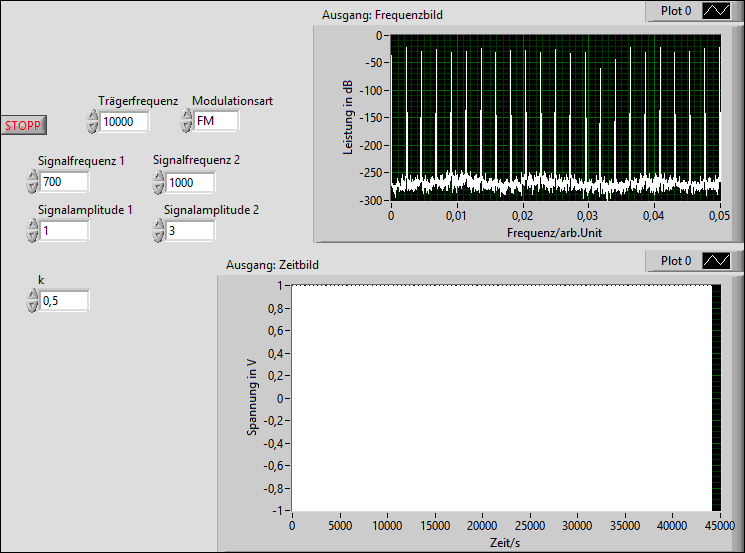
\includegraphics[width=1.0\textwidth]{EIRE2018Dateien/Tag4/FMPM-Erzeugung/anderekbei10000Traegerfr/FM-FMPM-Erzeugungp}
		\caption{In der Abbildung ist das Frontpanel bzw. die Benutzeroberfläche des LabVIEW-Programms zur Realisierung der Frequenzmodulation zu sehen. Der dabei betrachtete $k$-Wert ist sehr groß gewählt, weshalb die Peaks im Frequenzbild sehr stark ausgeprägt sind.}
		\label{FMAusgabegrossesk}
	\end{figure}
	
	\noindent Der Graph erscheint daher wie ein \glqq weißer Block\grqq\ aus Linien. 
	Der Vergleich der beiden Frequenzbilder zeigt, dass die Vergrößerung des $k$-Wertes zu schärfer definierten Peaks im Frequenzspektrum führt.
	Dies geht auch aus \cref{FMFormel} hervor.
	
	%PM-Absatz:
	Phasenmoduliert man das Signal $s(t)$, so nimmt das daraus entstehende PM-Signal $S_{PM}(t)$ die Form
	
	\begin{equation} \label{PMFormel}
	S_{PM}(t) = \cos (2\pi (f_0 t + k \cdot s(t)))
	\end{equation}
	
	\noindent an. 
	Dabei bildet $f_0$ die Trägerfrequenz und $t$ die Zeit. 
	$k$ ist ein fester, aber beliebig wählbarer Faktor. 
	Aufgrund der Ähnlichkeit von \cref{PMFormel} zu \cref{FMFormel}, verläuft auch die Realisierung der Phasenmodulation als LabVIEW-Programm ähnlich zur Programm-Umsetzung der Frequenzmodulation. 
	Daher besteht lediglich die Notwendigkeit, das für die Phasenmodulation reservierte, freie, ausfüllbare Case-Feld passend zu besetzen.
	
	\begin{figure}[H]
		\centering
		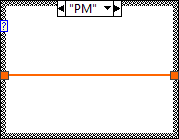
\includegraphics[width=0.6\textwidth]{EIRE2018Dateien/Tag4/FMPM-Erzeugung/PM-FMPM-Erzeugungd1}
		\caption{Es ist der in \cref{FMProgrammcode} nicht sichtbare Teil des LabVIEW-Programmcodes dargestellt, der notwendig ist, um die Art der Modulation auf der Benutzeroberfläche des Programms auszuwählen zu können. Bei diesem hier abgebildeten Programmcodeteil handelt es sich um eine weitere Option in der Case-Konstruktion, welche darauf abzielt die Phasenmodulation zu ergänzen.}
		\label{PMProgrammcode}
	\end{figure}
	
	\noindent Wie im Programmcode in \cref{PMProgrammcode} zu erkennen, wird hierbei die Leitung direkt durch das Case-Feld gezogen, ohne das übertragene Signal zu bearbeiten oder zu verändern. 
	In Kombination mit der bereits durch die Frequenzmodulation existierenden Programm-Struktur ist damit die Umsetzung der Phasenmodulation abgeschlossen. 
	
	\begin{figure}[H]
		\centering
		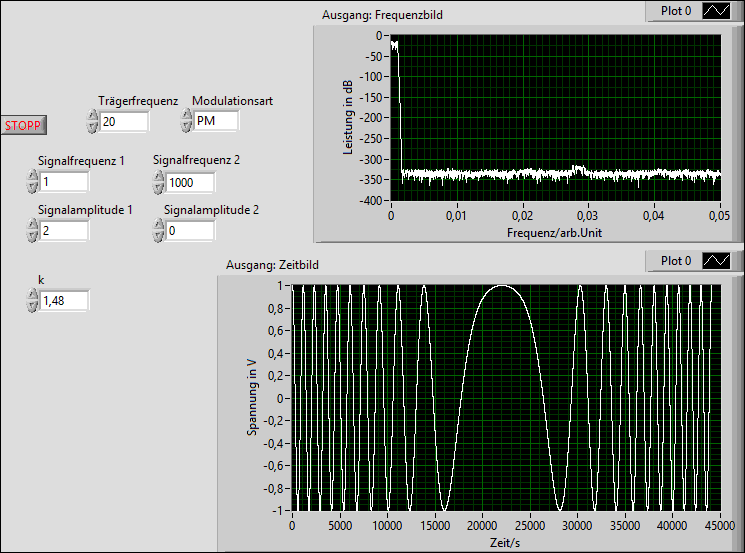
\includegraphics[width=1.0\textwidth]{EIRE2018Dateien/Tag4/FMPM-Erzeugung/PM-FMPM-Erzeugungp}
		\caption{Die Abbildung zeigt das Frontpanel bzw. die Benutzeroberfläche des LabVIEW-Programms zur Realisierung der Phasenmodulation.}
		\label{PMAusgabe}
	\end{figure}
	
	\noindent Das sich ergebene phasenmodulierte Signal $S_{PM}(t)$ sowie dessen Fourier-Transformierte $\tilde{S}_{PM}(f)$ sind in den beiden Diagrammen auf der Benutzeroberfläche des Programms in \cref{PMAusgabe} dargestellt.
	
	%Hinweis:
	\emph{Hinweis:} Bei diesem LabVIEW-Programm zur Erzeugung von phasen- und frequenzmodulierten Signalen ist zu beachten, dass zwischen den $k$-Werten der Frequenzmodulation und den $k$-Werten der Phasenmodulation stets eine Diskrepanz um einen Faktor der Größenordnung $10^4$ vorliegt.
	Denn dadurch ergeben sich für beide Modulationsarten die verlässlichsten Ergebnisse.
		
	
	
		
	\subsection{Demodulation eines phasen- bzw. frequenzmodulierten Signals} \label{FMPMDemodulation} %Bilderanordnung schön, bitte so lassen.
	
	
	%Allgemeiner Absatz:
	Im Folgenden soll ein von der Computer-Soundkarte ausgegebenes (im Hintergrund wird das in \cref{FMPMErzeugung} entstandene LabVIEW-Programm ausgeführt) und anschließend über den Analog-Digital-Wandler gemessenes Signal, welches entweder phasen- oder frequenzmoduliert wurde, demoduliert werden. 
	Der Programmcode des dafür erstellten LabVIEW-Programms ist in \cref{FMPMDemodProgrammcode1} und \cref{FMPMDemodProgrammcode2} zu sehen.
	
	\begin{figure}[H]
		\centering
		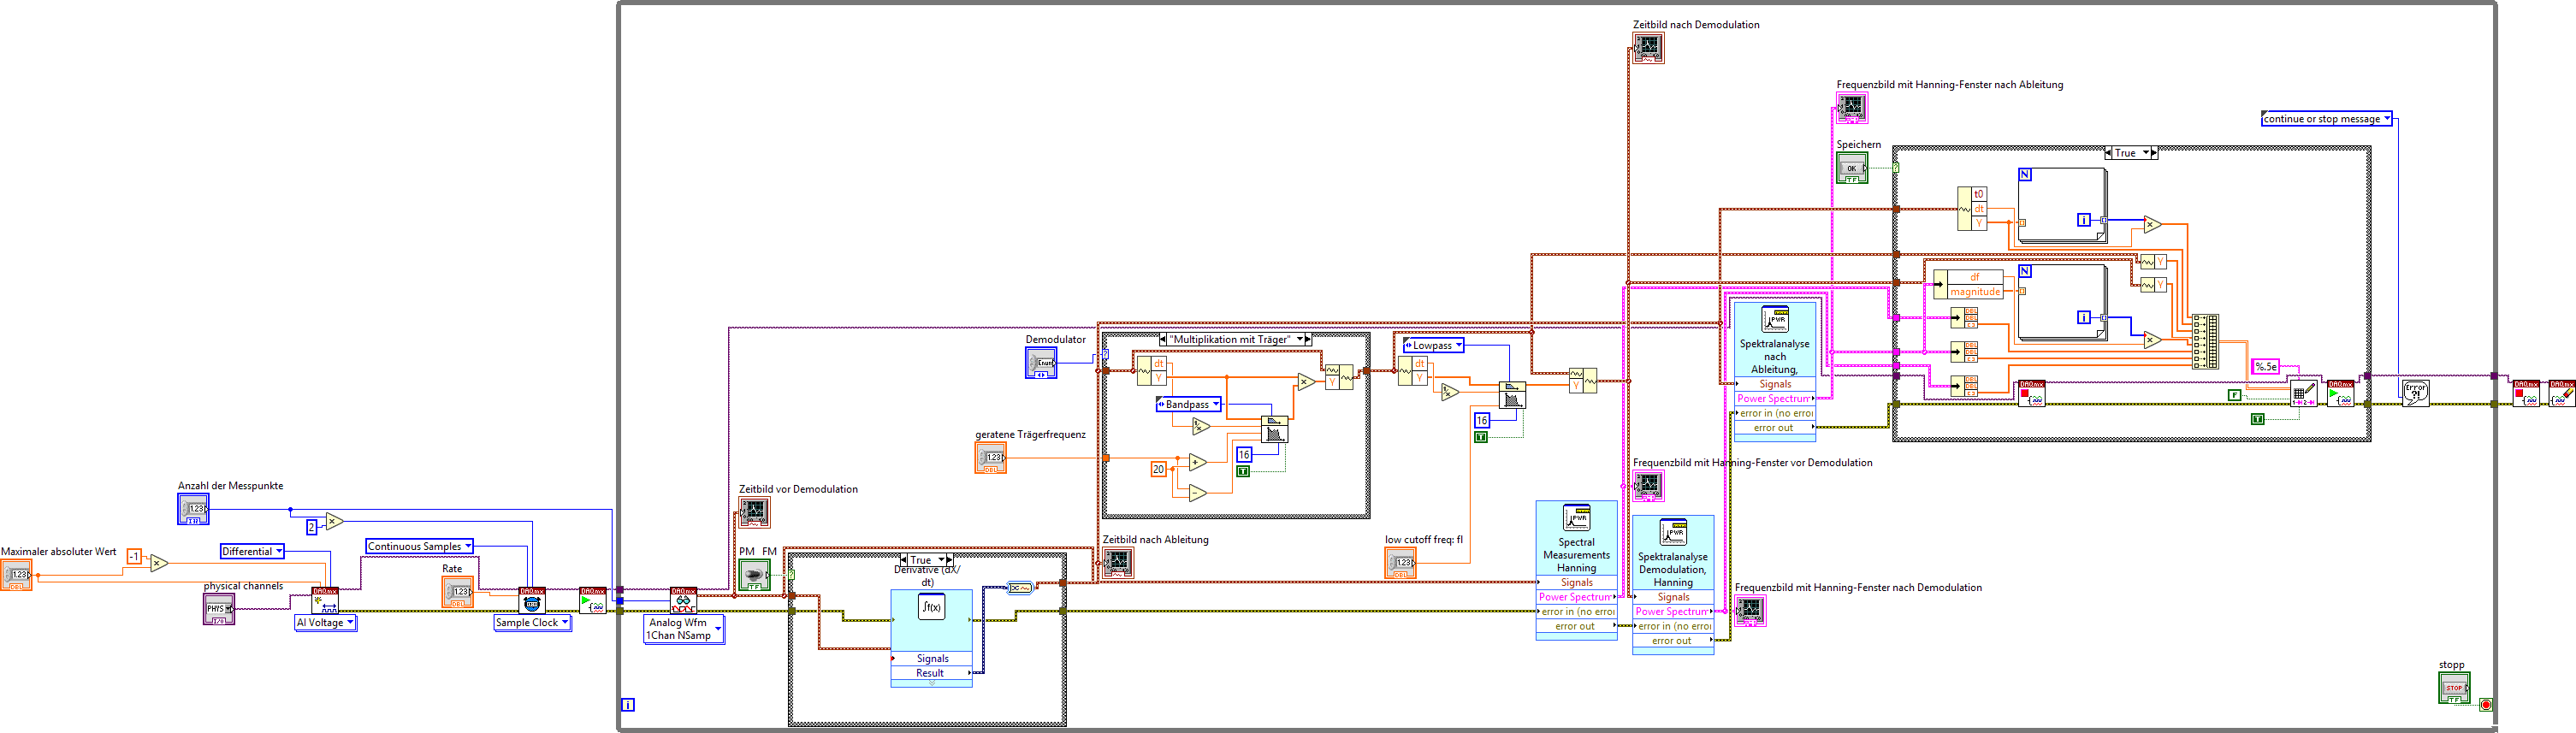
\includegraphics[width=1.0\textwidth]{EIRE2018Dateien/Tag4/OsziFMPM-Demod/FM/OsziPlusFMPMd}
		\caption{Die Abbildung veranschaulicht das LabVIEW-Blockdiagramm bzw. den Programmcode zur Demodulation eines von der Computer-Soundkarte ausgegebenen und anschließend über den Analog-Digital-Wandler gemessenen, phasen- bzw. frequenzmodulierten Signals.}
		\label{FMPMDemodProgrammcode1}
	\end{figure}
	
	\noindent Die \cref{FMPMDemodFrontpanel} zeigt das dazugehörige Frontpanel.
	Das in \cref{DemodTraeger} erhaltene LabVIEW-Programm dient dabei als Vorlage. 
	Von links nach rechts gelesen, beinhaltet dessen Programmcode, welcher in \cref{MultiTraegerProgrammcode} dargestellt ist, einen Programmteil zur Messdatenaufnahme mittels Analog-Digital-Wandler, einen für die Demodulation von AM-Signalen zuständigen Programmbereich, einen Tiefpassfilter sechzehnter Ordnung mit einer Grenzfrequenz von $1.600\,$Hz, einige Blockdiagrammobjekte zur Realisierung der Anzeige- bzw. Ausgabeelemente auf dem Frontpanel sowie eine Speicher- und eine Anhalte-Funktion für das Programm mit den entsprechenden \glqq Speichern\grqq - und \glqq Stopp\grqq -Knöpfen auf der Benutzeroberfläche.
	Mit den passenden Erweiterungen und Veränderungen des Programmcodes lässt sich nun die Demodulation eines von der Computer-Soundkarte ausgegebenen und anschließend über den Analog-Digital-Wandler gemessenen FM- bzw. PM-Signals umsetzen. 
	Dazu wird eine Case-Konstruktion zwischen dem Programmteil zur Messdatenaufnahme und dem Programmbereich für die Demodulation von amplitudenmodulierten Signalen hinzugefügt, welche insgesamt zwei Case-Optionen umfasst.
	Auf diese Weise entstehen zwei zunächst freie, ausfüllbare Case-Felder, wobei das Erste für die Frequenzmodulation und das Zweite für die Phasenmodulation vorgesehen ist.
	Der Wechsel zwischen diesen beiden Optionen findet dabei mit Hilfe eines sich auf der Benutzeroberfläche befindenden Kippschalters statt, welcher die der Case-Feld-Reservierungen entsprechenden Markierungen \glqq FM\grqq\ und \glqq PM\grqq\ besitzt.
	
	%FM-Absatz:
	Zur Demodulation eines gemessenen, frequenzmodulierten Signals wird die FM-Signalfunktion $S_{FM}(t)$ zunächst differenziert bzw. abgeleitet.
	Im Programmcode in \cref{FMPMDemodProgrammcode1} wird diese numerische Differentiation innerhalb des für die Frequenzmodulation reservierten Case-Feldes (\glqq FM\grqq ) realisiert.
	Das abgeleitete FM-Signal kann anschließend als AM-Signal betrachtet werden.
	Daher lässt es sich nun mit Hilfe einer der drei bereits aus \cref{DemodTraeger} bekannten und auch hier zur Verfügung stehenden AM-Demodulationsmethoden (\glqq Quadrat\grqq , \glqq Betrag\grqq\ und \glqq Multiplikation mit Träger\grqq ) demodulieren.
	
	\begin{figure}[H]
		\centering
		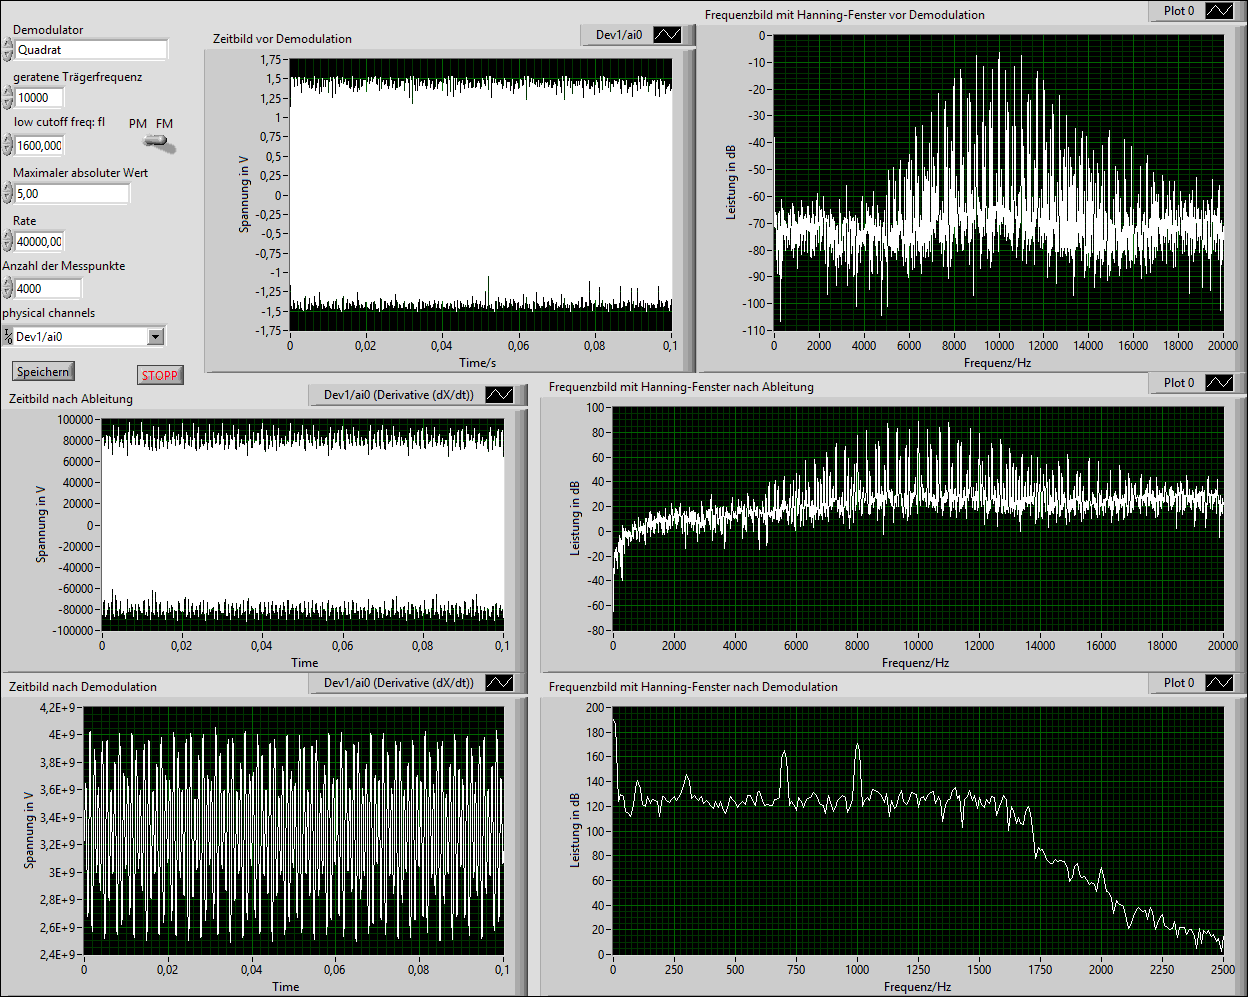
\includegraphics[width=1.0\textwidth]{EIRE2018Dateien/Tag4/OsziFMPM-Demod/FM/OsziPlusFMPMp}
		\caption{In dieser Abbildung ist die LabVIEW-Benutzeroberfläche bzw. das LabVIEW-Frontpanel des Programms zur Demodulation eines von der Computer-Soundkarte ausgegebenen und anschließend über den Analog-Digital-Wandler gemessenen, frequenzmodulierten Signals (\glqq FM\grqq ) dargestellt. Die AM-Demodulation findet hierbei mittels \glqq Quadrat\grqq -Methode statt.}
		\label{FMPMDemodFrontpanel}
	\end{figure}
	
	\noindent Anhand der auf dem Frontpanel in \cref{FMPMDemodFrontpanel} ersichtlichen Anzeigeelemente kann der Demodulationsprozess eines FM-Signals verfolgt werden:
	Die beiden oberen Diagramme bilden das Zeitbild und das Frequenzbild mit Hanning-Fenster des gemessenen FM-Signals vor der Demodulation.
	In der Mitte befinden sich zwei Diagramme, welche das Zeitbild und das Frequenzbild mit Hanning-Fenster des abgeleiteten FM-Signals veranschaulichen.
	Die beiden unteren Diagramme stellen das Zeitbild und das Frequenzbild mit Hanning-Fenster des demodulierten FM-Signals nach der Tiefpassfilterung dar.
	
	\begin{figure}[H] %FM-Diagramm
		\centering
		\includegraphics[width=1.0\textwidth]{EIRE2018Dateien/Tag4/OsziFMPM-Demod/FM/Frequenzbild_mit_Hanning_nach_TP_und_Demod_k0,005}
		\caption{Die Abbildung zeigt das Frequenzspektrum eines FM-Signals mit $k=0,005$ nach Abschluss der Demodulation und Tiefpassfilterung. Bei diesem Frequenzbild mit Hanning-Fenster handelt es sich um das Äquivalent zu dem aus \cref{FMPMDemodFrontpanel} bekannten, sich rechts unten befindenden Frontpanel-Diagramm. Die Daten für das hier dargestellte Frequenzspektrum entspringen der durch die Speicherfunktion des LabVIEW-Programms erhaltenen txt-Datei und wurden mit dem Datenanalyse-Programm \glqq SciDAVis\grqq\ bearbeitet. Die verwendete AM-Demodulation findet mittels \glqq Quadrat\grqq -Methode statt.}
		\label{FMDiagramm}
	\end{figure}
	
	\noindent Ebenjenes Frequenzbild mit Hanning-Fenster und das in \cref{FMDiagramm} zu sehende Diagramm bilden somit das Ergebnis der Demodulation des FM-Signals, anhand derer man auch erkennen kann, dass es sich um eine erfolgreich umgesetzte FM-Demodulation handelt.
	Denn die beiden deutlich sichtbaren Peaks im Frequenzspektrum liegen bei $700\,$Hz und $1.000\,$Hz, was genau den Frequenzen $f_1$ und $f_2$ des Signals $s(t)$ entspricht, welches es zu frequenzmodulieren galt.
	
	%PM-Absatz:
	Im Gegensatz zur FM-Demodulation wird bei der Demodulation eines gemessenen, phasenmodulierten Signals dieses PM-Signal von vornherein als AM-Signal betrachtet.
	Wie im Programmcodeteil in \cref{FMPMDemodProgrammcode2} zu sehen ist, werden die Leitungen daher direkt durch das für die Phasenmodulation reservierte Case-Feld (\glqq PM\grqq ) gezogen, sodass das übertragene Signal nicht verändert oder beeinflusst wird.
	
	\begin{figure}[H]
		\centering
		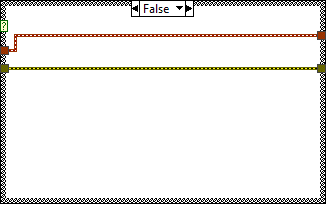
\includegraphics[width=0.6\textwidth]{EIRE2018Dateien/Tag4/OsziFMPM-Demod/PM/OsziPlusFMPMd5}
		\caption{In dieser Abbildung ist der in \cref{FMPMDemodProgrammcode1} nicht sichtbare Teil des LabVIEW-Programmcodes zu sehen, der notwendig ist, um auf der Benutzeroberfläche des Programms zwischen der Demodulation des FM-Signals und der Demodulation des PM-Signals wechseln zu können. Bei diesem hier abgebildeten Programmcodeteil handelt es sich um die zweite Option in der Case-Konstruktion, mit dessen Hilfe die Demodulation des phasenmodulierten Signals umgesetzt wird.}
		\label{FMPMDemodProgrammcode2}
	\end{figure}
	
	\noindent Dementsprechend durchläuft das PM-Signal anschließend eine AM-Demodulation nach den bereits erwähnten, verfügbaren AM-Demodulationsmethoden.
	\cref{PMDiagramm} zeigt das Ergebnis der Demodulation und Tiefpassfilterung des PM-Signals.
	
	\begin{figure}[H] %PM-Diagramm
		\centering
		\includegraphics[width=1.0\textwidth]{EIRE2018Dateien/Tag4/OsziFMPM-Demod/PM/Frequenzbild_mit_Hanning_nach_TP_und_Demod_k0,1}
		\caption{In dieser Abbildung ist das Ergebnis der Demodulation und Tiefpassfilterung eines PM-Signals mit $k=0,1$ zu sehen. Dieses Frequenzbild mit Hanning-Fenster ist das Äquivalent zu dem aus \cref{FMPMDemodFrontpanel} bekannten, sich rechts unten befindenden Frontpanel-Diagramm. Die Daten für das hier dargestellte Frequenzspektrum entspringen der durch die Speicherfunktion des LabVIEW-Programms erhaltenen txt-Datei und wurden mit dem Datenanalyse-Programm \glqq SciDAVis\grqq\ bearbeitet. Die verwendete AM-Demodulation findet mittels \glqq Quadrat\grqq -Methode statt.}
		\label{PMDiagramm}
	\end{figure}
	
	\noindent Da sich die beiden in diesem Frequenzspektrum deutlich sichtbaren Peaks bei $700\,$Hz und $1.000\,$Hz befinden und diese genau den Frequenzen $f_1$ und $f_2$ des Signals $s(t)$ entsprechen, kann man von einer erfolgreichen Demodulation des gemessenen, phasenmodulierten Signals sprechen.
	
	
	
	
	\subsection{Erweiterte Demodulation mit Bandpass und zusätzlicher Integration des Signals} %Bilderanordnung schön, bitte so lassen.
	
	%Allgemeiner Absatz:
	Da es sich hierbei um eine Programm- und Demodulationserweiterung handelt, bildet der in \cref{FMPMDemodulation} entstandene Programmcode die Basis für das folgende LabVIEW-Programm.
	Dessen Blockdiagramm ist in \cref{DemodIntBandProgrammcode1} und \cref{DemodIntBandProgrammcode2} dargestellt.
	
	\begin{figure}[H]
		\centering
		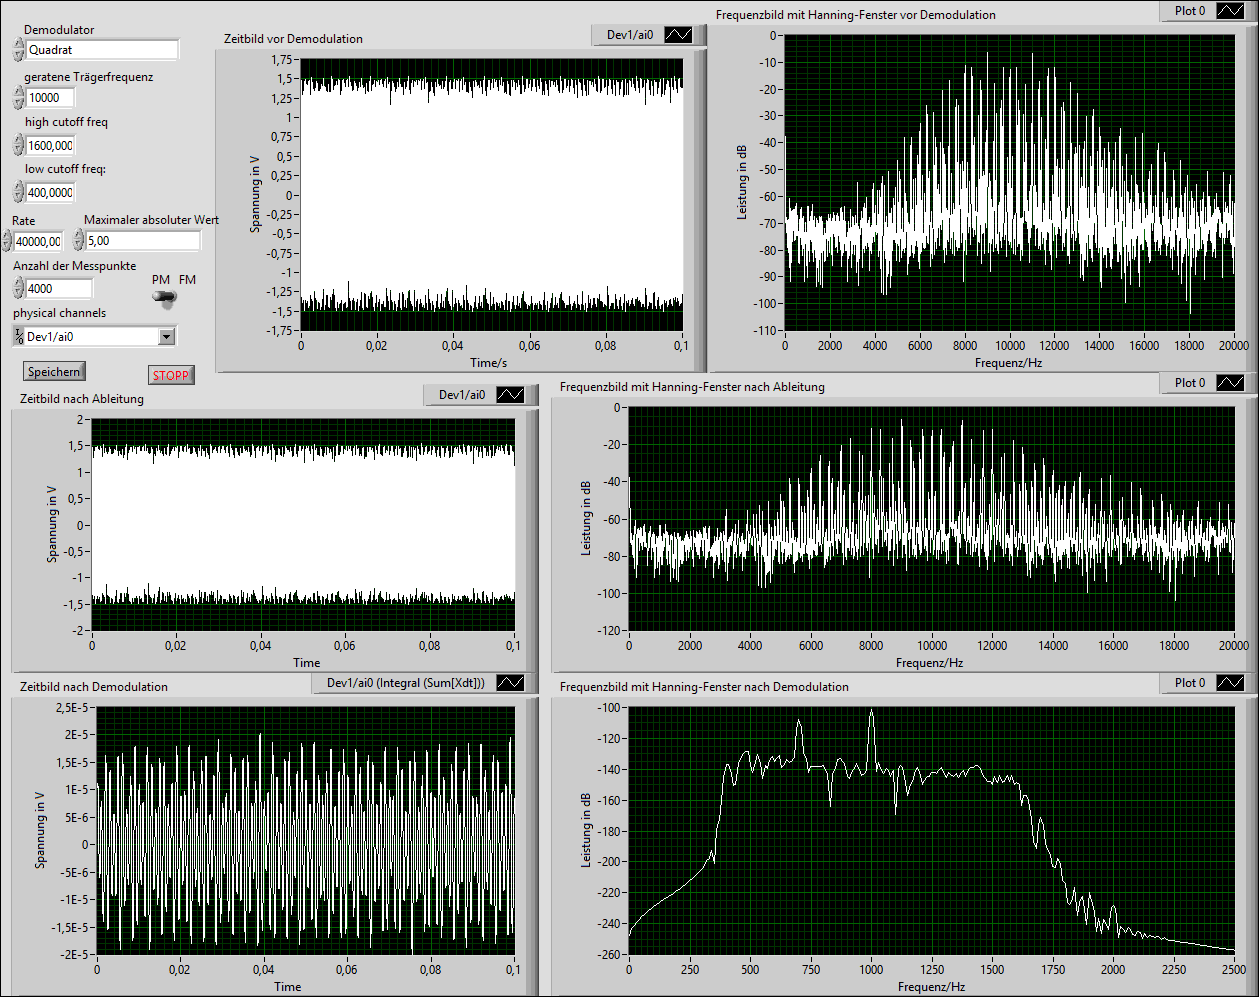
\includegraphics[width=1.0\textwidth]{EIRE2018Dateien/Tag4/OsziFMPM-Demod/mitBandpassUndIntegrationBilder/OsziPlusFMPMp}
		\caption{In dieser Abbildung ist die LabVIEW-Benutzeroberfläche bzw. das LabVIEW-Frontpanel des Programms zur erweiterten Demodulation eines von der Computer-Soundkarte ausgegebenen und anschließend über den Analog-Digital-Wandler gemessenen, phasenmodulierten Signals (\glqq PM\grqq ) dargestellt. Die AM-Demodulation findet hierbei mittels \glqq Quadrat\grqq -Methode statt.}
		\label{DemodIntBandFrontpanel}
	\end{figure}
	
	\noindent \cref{DemodIntBandFrontpanel} zeigt das dazugehörige Frontpanel.
	
	%Absatz zum Bandpass:
	Zunächst wird der der AM-Demodulation nachstehende Tiefpassfilter durch einen Bandpassfilter sechzehnter Ordnung ersetzt, was unter anderem im Programmcodeteil in \cref{DemodIntBandProgrammcode1} zu sehen ist.
	
	\begin{figure}[H]
		\centering
		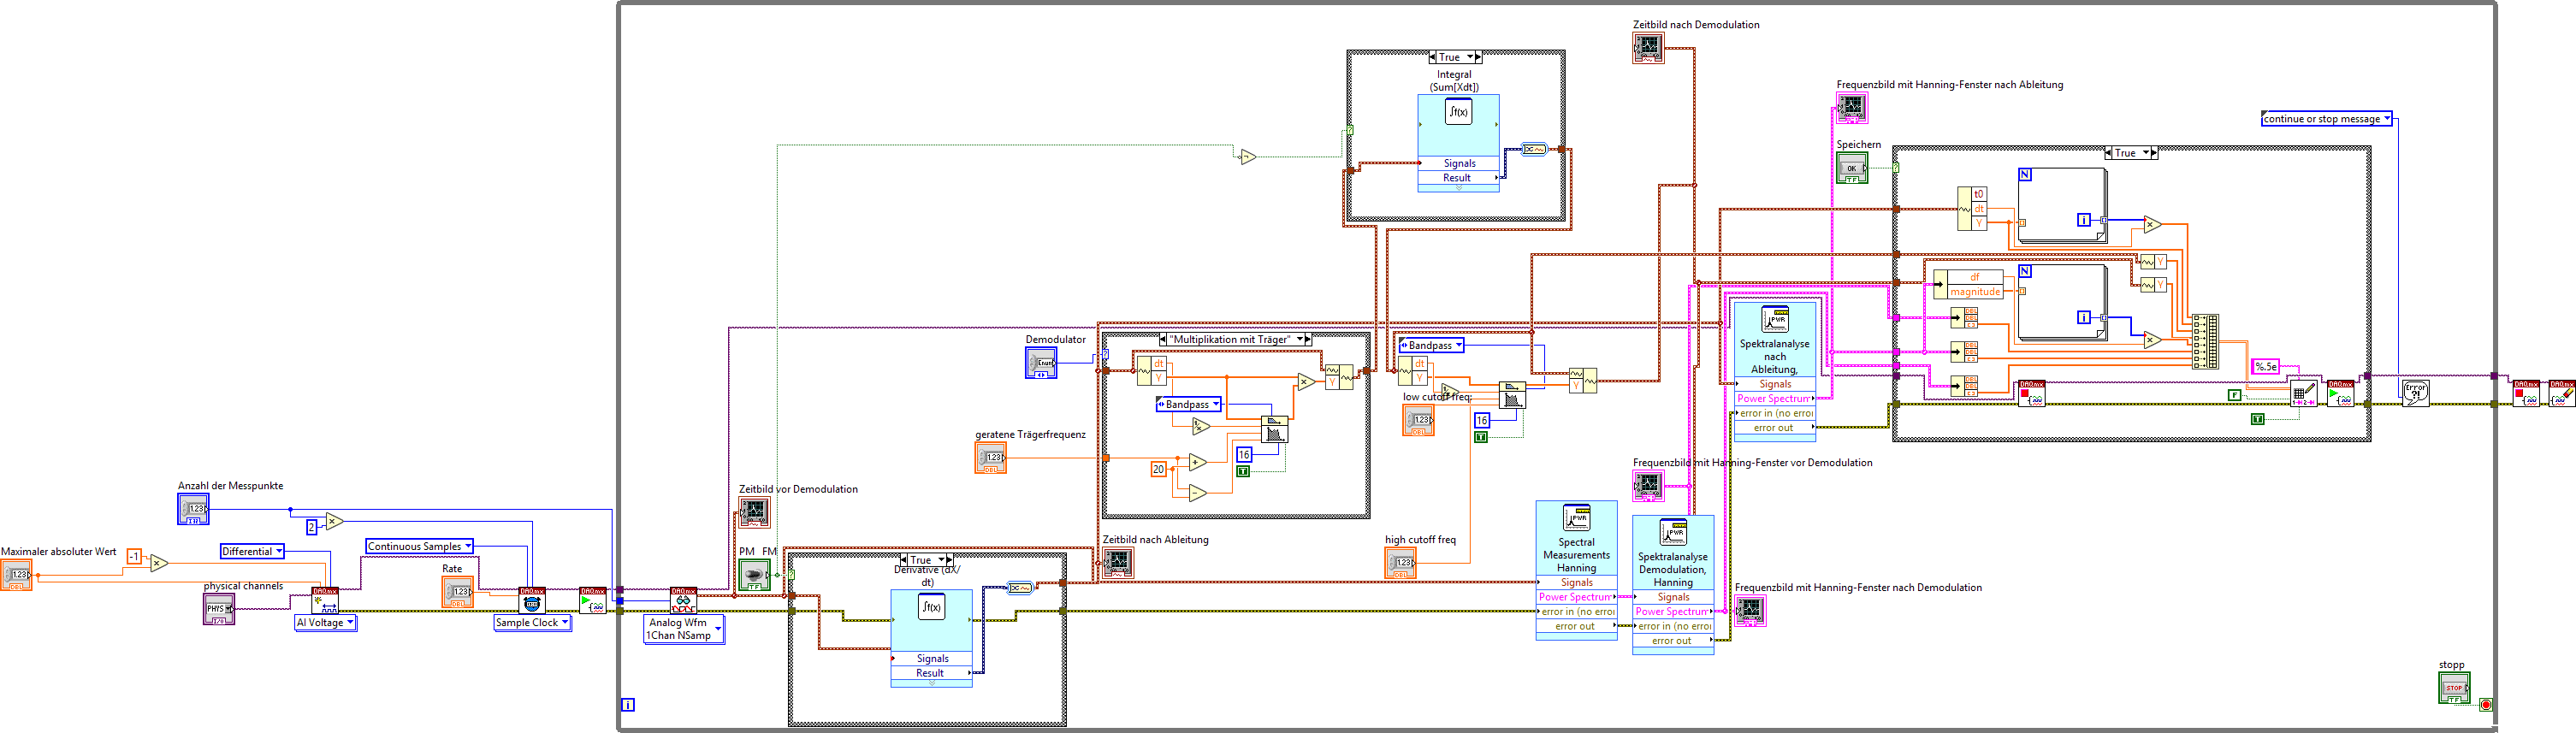
\includegraphics[width=1.0\textwidth]{EIRE2018Dateien/Tag4/OsziFMPM-Demod/mitBandpassUndIntegrationBilder/OsziPlusFMPMd}
		\caption{Die Abbildung veranschaulicht das LabVIEW-Blockdiagramm bzw. den Programmcode zur erweiterten Demodulation eines von der Computer-Soundkarte ausgegebenen und anschließend über den Analog-Digital-Wandler gemessenen, phasen- oder frequenzmodulierten Signals.}
		\label{DemodIntBandProgrammcode1}
	\end{figure}
	
	\noindent Die obere und untere Grenzfrequenz lässt sich dabei durch entsprechende auf dem Frontpanel hinzugefügte Bedienelemente einstellen.
	Die untere Grenzfrequenz soll $400\,$Hz und die obere Grenzfrequenz $1.600\,$Hz betragen.
	
	%Absatz zur Integration:
	Im Programmcode wird zwischen dem für die Demodulation von AM-Signalen zuständigen Programmbereich und dem Bandpassfilter eine Case-Konstruktion ergänzt, welche insgesamt zwei Case-Optionen umfasst.
	Dadurch entstehen zwei zunächst freie, ausfüllbare Case-Felder, wobei das Erste für demodulierte FM-Signale und das Zweite für demodulierte PM-Signale vorgesehen ist.
	Über eine Leitung mit NOT-Gate und in Verbindung mit dem bereits aus \cref{FMPMDemodulation} bekannten Kippschalter lässt sich die Case-Konstruktion ansteuern, sodass beim Weiterverfahren mit dem demodulierten Signal zwischen ursprünglich frequenzmodulierten Signalen und ursprünglich phasenmodulierten Signalen unterschieden werden kann.
	
	\begin{figure}[H]
		\centering
		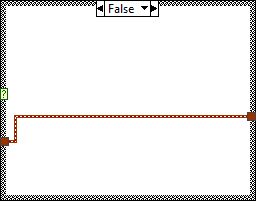
\includegraphics[width=0.6\textwidth]{EIRE2018Dateien/Tag4/OsziFMPM-Demod/mitBandpassUndIntegrationBilder/OsziPlusFMPMd6}
		\caption{In dieser Abbildung ist der in \cref{DemodIntBandProgrammcode1} nicht sichtbare Teil des LabVIEW-Programmcodes zu sehen. Dieser Programmcodeteil bildet die zweite Option in der Case-Konstruktion und sorgt dafür, dass das demodulierte FM-Signal vor der Bandpassfilterung nicht verändert wird.}
		\label{DemodIntBandProgrammcode2}
	\end{figure}
	
	\noindent Wie im Programmcodeteil in \cref{DemodIntBandProgrammcode2} zu erkennen ist, wird die Leitung direkt durch das für demodulierte FM-Signale reservierte Case-Feld gezogen, sodass das übertragene Signal unverändert bleibt.
	Innerhalb des für demodulierte PM-Signale reservierten Case-Feldes wird das Signal hingegen mit Hilfe der Simpsonregel numerisch integriert und anschließend an den Bandpassfilter weitergegeben.
	Dies ist im Programmcode in \cref{DemodIntBandProgrammcode1} zu sehen.
	Auf diese Weise verschwinden die Gleichanteile und die Frequenzabhängigkeit des demodulierten PM-Signals.
	
	\begin{figure}[H] %FM-Diagramm mit Bandpass
		\centering
		\includegraphics[width=1.0\textwidth]{EIRE2018Dateien/Tag4/OsziFMPM-Demod/FMmitBandpassundInt/Frequenzbild_mit_Hanning_nach_BP_und_Demod}
		\caption{In dieser Abbildung ist das Ergebnis der Demodulation und Bandpassfilterung eines FM-Signals zu sehen. Dieses Frequenzbild mit Hanning-Fenster ist das Äquivalent zu dem aus \cref{DemodIntBandFrontpanel} bekannten, sich rechts unten befindenden Frontpanel-Diagramm. Die Daten für das hier dargestellte Frequenzspektrum entspringen der durch die Speicherfunktion des LabVIEW-Programms erhaltenen txt-Datei und wurden mit dem Datenanalyse-Programm \glqq SciDAVis\grqq\ bearbeitet. Die verwendete AM-Demodulation findet mittels \glqq Quadrat\grqq -Methode statt.}
		\label{FMIntBandDiagramm}
	\end{figure}
	
	\noindent Das Ergebnis der erweiterten Demodulation sowie Bandpassfilterung eines von der Computer-Soundkarte ausgegebenen und anschließend über den Analog-Digital-Wandler gemessenen FM- bzw. PM-Signals ist in \cref{FMIntBandDiagramm} bzw. \cref{FMIntBandDiagramm} als Diagramm dargestellt.
	In diesen beiden Frequenzspektren lassen sich zwei deutliche Peaks bei $700\,$Hz und $1.000\,$Hz ausmachen.
	
	\begin{figure}[H] %PM-Diagramm mit Bandpass und Integration 
		\centering
		\includegraphics[width=1.0\textwidth]{EIRE2018Dateien/Tag4/OsziFMPM-Demod/PMmitBandpassundInt/Frequenzbild_mit_Hanning_nach_BP,Int,Demod}
		\caption{Die Abbildung zeigt das Frequenzspektrum eines PM-Signals nach Abschluss der Demodulation, Integration und Bandpassfilterung. Bei diesem Frequenzbild mit Hanning-Fenster handelt es sich um das Äquivalent zu dem aus \cref{DemodIntBandFrontpanel} bekannten, sich rechts unten befindenden Frontpanel-Diagramm. Die Daten für das hier dargestellte Frequenzspektrum entspringen der durch die Speicherfunktion des LabVIEW-Programms erhaltenen txt-Datei und wurden mit dem Datenanalyse-Programm \glqq SciDAVis\grqq\ bearbeitet. Die verwendete AM-Demodulation findet mittels \glqq Quadrat\grqq -Methode statt.}
		\label{PMIntBandDiagramm}
	\end{figure}
	
	\noindent Diese entsprechen genau den Frequenzen $f_1$ und $f_2$ des zu modulierenden Signals $s(t)$, weshalb man von einer erfolgreich umgesetzten, erweiterten Demodulation und Bandpassfilterung des gemessenen, frequenzmodulierten bzw. phasenmodulierten Signals sprechen kann.
		
	%Hinweis:
	\emph{Hinweis:} Sobald $k$ innerhalb eines bestimmten Wertebereichs liegt, werden die sich nach der erweiterten Demodulation und Bandpassfilterung eines FM- bzw. PM-Signals ergebenen Frequenzspektren anschaulicher und die Peaks sind deutlicher zu erkennen.
	Ist der $k$-Wert jedoch zu hoch, kommen zu viele Oberwellen zustande.
	Wenn der $k$-Wert wiederum zu klein gewählt wird, verschwindet das demodulierte Signal im Hintergrundrauschen.
	
	
	
	\printbibliography
	
	
\end{document}
